\chapter{Neuron Modeling Software}
\label{chap:software-modeling-Neurons}

For parameter search, read Chap.\ref{chap:parameter-search}.

Simulating a neural model means tracking the change of neural
variables such as membrane potential or synaptic weights over
time.

The rules governing these changes take two principal forms:
\begin{enumerate}
  
  \item  {\bf continuous updates} (e.g., the decay of the membrane potential
  back to a resting state in the absence of inputs) and 

continuous updates can be described by deterministic
or stochastic differential equations
  
  \item {\bf event-based updates} (e.g., the reset after a spike in an
  integrate-and-fire neuron, or the impact of a pre-synaptic spike on a
  post-synaptic cell) 

event-based updates can
be described as a series of mathematical operations
\end{enumerate}




\section{Community efforts}

Computational models are often developed from custom-developed software.
Efforts to make them exchangable from one tool to another is developing formal
language to describe models
\begin{enumerate}
  \item SBML [7] - Sect.\ref{sec:SBML}
  
  \item CellML [8],
  
  \item NeuroML
\end{enumerate}

and ontologies to describe components in a model if they are the same from two
models, ragardless of names being used.
\begin{enumerate}
  \item  BioPAX [9] 
\end{enumerate}


List:
\url{https://grey.colorado.edu/emergent/index.php/Comparison_of_Neural_Network_Simulators}

MatLab is better generally, but of course everything has to be made from
scratch. For modelling signals and their generation it is clearly superior, but
difficult, of course, for more anatomically oriented modelling where Neuron is
best.

NEST (Sect.\ref{sec:NEST}) and Brian (Sect.\ref{sec:Brian}) are best to simulate
spiking neuronal networks. To simulate rate-coded neuronal network, we can use
ANNarchy (Sect.\ref{sec:ANNarchy}).

NEURON and GENESIS (Sect.\ref{sec:GENESIS}) are excellent references (for cell
scale , small networks or complex ionic mechanisms simulations) but if you are
looking for large-scale simulators where simple models of neurons are often
used, the Brian simulator is perfect.

An effort to create a software-neutral model description format include NeuroML
(Sect.\ref{sec:NeuroML-file-format}). A neuron model built with or converted to
NeuroML should be able to run on Neuron, Genesis, and plenty of other platforms.

\subsection{Human-brain project (hardware-based)}

\url{http://www.artificialbrains.com/human-brain-project}

This is a EU-funded project to
 build a complete, biologically realistic, simulation of the human brain within
a supercomputer.
\url{https://www.humanbrainproject.eu/}

\subsection{Particle-based simulator}
\label{sec:particle-based-simulator}

The  dominant  particle  based  simulators  are  ChemCell 
(Sect.\ref{sec:ChemCell}), MCell  (Sect.\ref{sec:MCell}),  and  Smoldyn
(Sect.\ref{sec:Smoldyn}).

ChemCell has the least feature, but is easy to use.

\subsection{spatial and stochastic}

Andrews - Arkins (2011)

\section{ANNarchy (rated-coded neural network)}
\label{sec:ANNarchy}

NNarchy (Artificial Neural Networks architect) neural simulator, which allows to
easily define and simulate rate-coded and spiking networks, as well as
combinations of both.

Rate-coded networks, however, do not benefit much from the advances of spiking
simulators. Rate-coded neurons do not communicate through discrete spike events
but through instantaneous firing rates (real values computed at each step of the
simulation). Rate-coded simulators are either restricted to classical neural
networks (static neurons learning with the backpropagation algorithm) or
optimized for particular structures such as convolutional networks.
The goal of ANNarchy is to provide a rate-coded simulator with a flexibility
similar to what Brian proposes.

The interface in Python has been designed to be close to the PyNN interface
(Sect.\ref{sec:PyNN}), while the definition of neuron and synapse models can be
specified using an equation-oriented mathematical description similar to the
Brian neural simulator (Sect.\ref{sec:Brian}).

This information is used to generate C++ code that will efficiently perform the
simulation on the chosen parallel hardware (multi-core system or graphical
processing unit). Several numerical methods are available to transform ordinary differential equations
into an efficient C++ code.


\section{AgentCell}
\label{sec:AgentCell}



AgentCell is an agent-based model of cellular biochemical processes and biological behavior.

\url{http://emonet.biology.yale.edu/software#agentcell}

\section{BioNetGen}
\label{sec:BioNetGen}

BioNetGen uses model-specification language (BNGL) - Sect.\ref{sec:BNGL} for
rule-based model development. 

A modeler specifies molecules, their interacting and modification domains, such
as tyrosines and SH2 domains, and rules of activities and interactions among
domains and molecules. Rules are used to automatically generate a model in the
form of a reaction network comprised of all chemical species corresponding to
specified molecules, and all transitions among these species, thus freeing the
user from the intense bookkeeping that would be required to enumerate such a
network by hand.



\section{Biographer}
\label{sec:biographer}

\url{https://code.google.com/archive/p/biographer/}




\section{Brian and Brian2 (neural network)}
\label{sec:Brian}
\label{sec:Brian2}

A full specification of such a network model includes a description of
the dynamics and state changes of neurons and synapses, as well as the synaptic
connectivity patterns and the initial values of all parameters.


Brian is a clock driven simulator for spiking neural networks, written in
Python.
The idea is that it can be used at various levels of abstraction without the
steep learning curve of software like Neuron (Sect.\ref{sec:NEURON}), where you
have to learn their own programming language to extend their models.

\url{http://www.briansimulator.org/docs/introduction.html}



\section{ChemCell}
\label{sec:ChemCell}


\section{Cytoscape}
\label{sec:Cytoscape}

Cytoscape:  visualizing molecular interaction networks and biological pathways
and integrating these networks with annotations, gene expression profiles and
other state data.

Cytoscape core distribution provides a basic set of features for data
integration, analysis, and visualization. Additional features are available as
Apps (formerly called Plugins). 

\url{http://www.cytoscape.org/what_is_cytoscape.html}

\section{DBSolveOptimum }
\label{sec:DBSolve}
\label{sec:DBSolveOptimum}

DBSolveOptimum  is  a succession and extension of DBSolve 5 and DBSolve 7; with
new tools for extended data analysis and multiple simulations: virtual clinical
trials and application of modern modeling techniques, like quantitative systems
pharmacology, to problems arising in drug research and development: both systems
pharmacology and conventional PK/PD models of drugs.



\url{http://insysbio.ru/en/software/db-solve-optimum}

\section{Ephus, ScanImage}
\label{sec:ScanImage}
\label{sec:Ephus}

Ephus and ScanImage are a set of software applications, mostly written in
MATLAB, for two-photon laser scanning microscopy, electrophysiology, laser
scanning photostimulation, and other important techniques in neurobiology. This
software has been developed at Cold Spring Harbor Laboratory and Janelia Farm
Research Campus.

Ephus is a collection of small programs which work together harmoniously to
support electrophysiology, LSPS, and other applications. 

Ephus and ScanImage interface to a growing range of hardware devices.
Frequently, custom software interfaces to these devices must be developed,
allowing their capabilities to be accessed via scripting in Matlab.

DABS: Dabs is a MATLAB package of hardware adapter classes, making device
capabilities available within MATLAB. ScanImage releases use and include the
current version of Dabs.

\url{https://openwiki.janelia.org/wiki/pages/viewpage.action?pageId=4390958}

\url{http://www.hhmi.org/research/circuit-and-synaptic-mechanisms-underlying-experience-dependent-cortical-plasticity}

\section{E-Cell}
\label{sec:E-Cell}



\url{http://www.e-cell.org/}

\section{jLEMS}
\label{sec:jLEMS}

jLEMS is Java Interpreter for the Low Entropy Model Specification language.

\url{https://github.com/LEMS/jLEMS}

\section{JDesigner}

JDesigner is a Win32 application which allows one to draw a biochemical network
and export the network in the form of SBML.
\url{http://sbw.kgi.edu/software/jdesigner.htm}

It has its own language and also support modleing tools (Sect.\ref{sec:Jarnac}).

\section{Libneurosim}
\label{sec:libneurosim}

Linneurosim is where standard APIs: ConnectionGenerator APIs
to support efficient generator of network connectivity during model setup
in neural network simulators. It was originally developed to support
libcsa from NEST (Sect.\ref{sec:NEST}).

Any simulator can use a library providing ConnectionGenerator
interface. 

\section{MCell}
\label{sec:MCell}

MCell is a Monte Carlo Simulator of Cellular Microphysiology - 
a realistic simulation of cellular signaling in the complex 3-D subcellular
microenvironment in and around living cells.

At such small subcellular scales the familiar macroscopic concept of
concentration is not useful and stochastic behavior dominates, i.e. individual
molecules are being tracked. 
MCell uses highly optimized Monte Carlo algorithms to track the stochastic
behavior of discrete molecules in space and time as they diffuse and interact
with other discrete effector molecules (e.g. ion channels, enzymes,
transporters) heterogeneously distributed within the 3-D geometry of the
subcellular environment.

MCell can generate outputs to a varity of formats, e.g. 3D images to be rendered
with IBM Data Explorer (www.opendx.org), or the companion visualization package
DReAMM (www.mcell.psc.edu/DReAMM).

\url{http://www.mcell.cnl.salk.edu}

\url{http://mcell.org/}

\section{MUSIC (MUltiSimulation Coordinator)}
\label{sec:MUSIC-Multisimulation-coordinator}

MUSIC is an API (written in C++) allowing large scale neuron simulators using
MPI internally to exchange data during runtime.  MUSIC provides mechanisms to
transfer massive amounts of event information and continuous values from one
parallel application to another.

In particular, MUSIC handles data transfer between applications that use
different time steps and different data allocation strategies.

A MUSIC-aware simulator links against the C++ library (libmusic.a) and can be
launched using mpirun together with the music utility as described below.  MUSIC
can also be used from a C program using the API in music-c.h.

MUSIC also has a utility: \verb!music!. 
A MUSIC multisimulation is specified in a configuration file given as
the first argument to the \verb!music! utility. Example:
\begin{verbatim}
cd test
mpirun -np 4 /usr/local/bin/music demo.music
\end{verbatim}


{\bf NOTE}: The typical usage cases are connecting models developed for
different simulators and connecting a parallel simulator to a post-processing
tool. A visualization tool \verb!viewevents! can be built if the GLUT toolkit is
installed.


{\bf NOTE}: MUSIC version 1.0 makes use of the "long long" data type supported
by, for example, the GNU C++ compiler g++.

{\bf NOTE}: Three simulators currently have MUSIC interfaces: Moose, NEURON and
NEST.


\url{https://github.com/INCF/MUSIC}

\url{https://github.com/INCF/MUSIC/issues/27}

\section{MOOSE}
\label{sec:MOOSE}

MOOSE (Multi-scale Object-Oriented Simulation Environment) is 
a completely re-written of GENESIS (Sect.\ref{sec:GENESIS}) with objects (e.g.
compartments) from Genesis are re-implemented with the same equations and names
in MOOSE. The major changes:
\begin{itemize}
  \item interface and numerics are completely different
  
It has a scripting interface with Python (Sect.\ref{sec:PyMoose}), graphical
displays with Matplotlib, PyQt, and OpenGL, and support for many model formats. 
  

  \item Biological concepts are mapped to classes
  
  A model is built by creating instances of these classes; and connect them by
  messages. 
  
  \item INPUT FORMAT: SBML (biochemical reaction specification), NeuroML
  (neural model specification), cell.p (neuron morphology specification)

MOOSE can read kinetic models in SBML (Sect.\ref{sec:SBML}) and GENESIS kkit
formats, from BioModels.net and DOQCS. MOOSE also supports electrical models specified in
NeuroML and Genesis .p formats, and can load over 30,000 morphology files from
NeuroMorpho.org (.swc format).

   \item OUTPUT FORMAT: HDF5
   
   
\end{itemize}

MOOSE is designed to simulate neural systems ranging from subcellular components
and biochemical reactions to complex models of single neurons, circuits, and
large networks.


\url{https://moose.ncbs.res.in/?q=documentation}

\subsection{PyMoose}
\label{sec:PyMoose}

In Moose, everything is organized as a tree structure with '/' as the root.

{\bf PyMoose}
\begin{verbatim}
import moose
help(moose)

dir(moose)     # list functions + classes

moose.le()   # list existing objects under '/' - the top of 
             # element hierarchy
             # /Msgs
             # /clock
             # /classes
             # /postmaster
             # NOTE: each object can contain other objects inside
             # element hierarchy is similar to organization of files on Linux 
             #  environment 
             #   Network(top) - Cell[1] -- Soma
                                        -- Dendrite[1]
             #                - Cell[2]
moose.le('/classes')  # list classes ~ Genesis listobjects command

# moose.doc(objectname)   #
moose.doc(moose.Compartment)
help(moose.Compartment) 
\end{verbatim}

Example: 
\begin{lstlisting}
  # create an instance from a given class object
  # you define a name to it
soma = moose.Compartment('/soma')  # create

  # the instance can be references via the returned name or directly
  # using moose.element('/soma')
  # '/soma' is the moose element path
  moose.le('/')  # to find the name
  soma = moose.element('/soma')  # select
  
  # Neutral is a special class object
neuron = moose.Neutral('/neuron')
soma = moose.Compartment('/neuron/soma')
dend = moose.Compartment('/neuron/dend')

data = moose.Neutral('/data')  
\end{lstlisting}


\subsection{fields of an element: moose.showfield()}

We have learnt how to create an element (Sect.\ref{sec:PyMoose}), each element
comes with many field
\begin{verbatim}
('this', 'name', 'me', 'parent', 'children', 'path', 'class', 'linearSize', 
'objectDimensions', 'lastDimension', 'localNumField', 'pathIndices', 'msgOut', 
'msgIn', 'Vm', 'Cm', 'Em', 'Im', 'inject', 'initVm', 'Rm', 'Ra', 'diameter', 
'length', 'x0', 'y0', 'z0', 'x', 'y', 'z')
\end{verbatim}
Some are for internal use, and some give accesses to physical properties (of
the biological entity) in that default values are populated
\begin{verbatim}
>>print soma.Cm, soma.Rm, soma.Vm, soma.Em, soma.initVm 
1.0 1.0 -0.06 -0.06 -0.06

>> moose.showfield('soma')

soma.Cm = 1e-9  # we can modify the value of a field
\end{verbatim}

{\bf UNITS}: There are no unit associated with the value. It is up to the user
to use a consistent set of units based on either (1) SI units; (2) physiological
units.

\begin{verbatim}
Physiological units, e.g. nanoAmps, Megaohms, nanoFarads, msec

current * resistance = volts
nA (10^-9) * Mohms (10^6) = mV (10^-3)

capacitance * resistance = time
nF(10^-9) * Mohms(10^6) = msec
uF (10^-6) * Mohms (10^6) = sec


=====================================
SI units

A method for working in SI units that appear physiological is to specify values
with e3, e-6, etc.  In other words, specify values using Xe6 for megaohms, Ye-6
for microSiemans, Ze-9 for nanoAmps, etc.  Then, you use SI units, but X, Y and
Z are the physiological values   

Length units and concentration units
Meters for SI, but 1 Meter^3 doesn't produce 1 Liter! It produces 1000 Liters
Thus, 1 mole in 1 meter cubed = 1 mM, so mM is an SI unit.
Also, microns are often used for morphology
\end{verbatim}


\subsection{connect elements: moose.connect}

This \verb!moose.connect()! send value/field from source to correct field in
destination. The message can be bi-direction. 

\begin{verbatim}
pulse = moose.PulseGen('pulse'
moose.showfield('pulse')
pulse.delay[0]   # first-delay
pulse.width[0]
pulse.level[0]
pulse.delay[1]


m=moose.connect(pulse, 'output', soma, 'injectMsg')
\end{verbatim}



\section{NEURON software}
\label{sec:NEURON}

NEURON has 2 components
\begin{enumerate}
  \item iv = InterView (for the GUI, only use for single machine)
  
  \item nrn = the NEURON simulator (can be used for a cluster of workstations
  or supercomputers) - Sect.\ref{sec:nrn-NEURON}
  
\end{enumerate}
\url{http://pub.ist.ac.at/~jguzman/doc/_sources/neuron/tutorial/Tutorial0.txt}

Preinstall
\begin{verbatim}
sudo apt-get install automake libtool libX11-dev 
sudo apt-get install xfonts-100dpi

\end{verbatim}

\subsection{source}

NEURON software comprise several programs, in that the main executable is
\verb!nrniv! 

\begin{enumerate}
  \item Random123
  
  \item {\bf nrniv} : the folder contains code to build \verb!nrniv! which
  contains the \verb!hoc! interpreter (and all of its extensions)
  
  
\end{enumerate}

\subsection{-- src/oc}
\label{sec:oc-interpreter}

The bare (C-based language) interpreter: \verb!oc! [no GUI, no neuron-specific
functions], which is used in NEURON v3. To support C++ classes and graphical
interfaces, we use \verb!ivoc! (which is written in C++).
 
This version of the hoc-based interpreter is introduced with object syntax that
allows much better structuring of the conceptual pieces that are assembled to
build a simulation.
 
\begin{verbatim}
main()                 : oc/ocmain.c
  hoc_main1()          : oc/hoc.c
     #if PVM           //parallel-virtual-machine?
        init_parallel()
     #fi
     
     hoc_audit_from_hoc_main1()
     hoc_main1_init();       //IMPORTANT
          while (moreinput())
          {
             hoc_run1();
                  |
                  /* initcode() <- initialize for code generation*/
                  /* hoc_yyparse() <- parse input code */
                  /* execute(..)   <- run the subprogram parsed */
                  for (initcode(); hoc_yyparse(); initcode())
                  {
                     execute(progbase); /* Inst *progbase 
                                      which is start of current subprogram */
                  }
          }     
     
\end{verbatim}
NOTE: \verb!hoc_run1()! call \verb!hoc_yyparse()!
\begin{verbatim}
void execute(Inst* p); /* run the machine, i.e. single statement or subprogram */
{
  
}
\end{verbatim}

Once \verb!oc! binary is run, it returns a command-line based interpreter, then
user can type in a name and arguments. The mapping from name to a
keyword or a function to execute is given in \verb!oc/hoc_init.c! file. The
names thus are classified into different groups

\begin{verbatim}
// names as keywords
'proc'     parsePROC
'func'     FUNC
'obfunc'   HOCOBJFUNC
'return'   RETURN
'break'    BREAK
'continue' CONTINUE
'stop'     STOPSTMT
'if'       IF
'else'     ELSE
'read'
'debug'
'double'
'em'
'depvar'
'eqn'
'local'
'localobj'
'strdef'
'parallel'    PARALLEL
'help'
'iterator'    ITERKEYWORD
'iterator_statement'    ITERSTMT

  //some for cable-equations
'create'        SECTIONKEYWORD
'connect'
'setpointer'
'access'
'insert'
'uninsert'
'forall'
'ifsec'
'forsec'

  //some for object-oriented
'begintemplate'
'end'template'
'objectvar'
'objref'
'public'
'external'
'new'

  //name as constant
'PI'          3.14159
'E'           2.718
'GAMMA'
'DEG'         57.29577    /* deg/radian */
'PHI'         1.6180339   /* golden ratio */
'FARADAY'
'R'
0

// names as functions (1 argument)
'sin'
'cos'
'atan'
'tanh'
'log'
'log10'          Log10
'exp'            hoc1_Exp 
'sqrt'           Sqrt    
'int'            integer

'quit'         hoc_quit
'secname'      hoc_secname
'units'        hoc_Symbol_units

// names as functions (multiple or variable arguments)



//strfunc_bltin       --> functions that returns a string
'getcwd'       hoc_getcwd

\end{verbatim}

All of the mapping from name/keyword-function is stored in \verb!struct Symbol*!
object.
\begin{verbatim}
typedef struct Symbol {
  char *name;
  short type;
  short subtype; /* flag for user integers */
  
  short cpublic;  /* flag telling if public variable in C */
  short public;  /* flag telling if public variable in C++ */
  
  short defined_on_the_fly;
  union {
  
      double* pval;  /* alias to scalar or user-defined double */
      struct {
         struct {
            /* machine instruction list type */
            /* FUNCTION, PROCEDURE, FUN_BLTIN */
            Pfrv pf;   /* typedef int (*Pfri)(void)  <-  pointer to function return int*/
             
            Pfrd pfd;
            Pfro pfo;
            Pfrs pfs;
            Pfrv_vp  pfv_vp;
            Pfrd_vp  pfd_vp;
            Pfro_vp  pfo_vp;
            Pfrs_vp  pfs_vp;
            HocUnion Inst *in;
            HocStruct Symbol *sym;
            void *ptr;
            int i;
         } defn;
         /* Inst defn */
         
         unsigned long size;
         HocStruct Symlist    *list; /* for constants and string*/
         
         int nauto;  /* # number of local variables */
         int nobjauto; /* the last of these are pointers to objects */
      }   u_proc;
      /* Proc *u_proc; */
    
  } u;
  
  unsigned s_varn;     /* if a dependent variable, 0 means indep */
  Arrayinfo   * arrayinfo;    /* ARRAY information, if NULL then scalar */
  HocSymextension*   extra;     /* additional symbol */
  
  HocStruct Symbol  *next;       /* link to next Symbol */
} Symbol;


Symbol* s;
\end{verbatim}

\subsection{-- src/ivoc}
\label{sec:ivoc-interpreter}



\subsection{neuron spatial discretization: neurite}
\label{sec:neurite}

An unbranched portion of a neuron is called a {\bf neurite} which can be
straight line or not, Fig.\ref{fig:NEURON_section-segments}(A). 

Tools to works with neurite:
\begin{itemize}
  \item NeuriteIQ - \ref{sec:NeuriteIQ}
  \item NeuriteQuant - \ref{sec:NeuriteQuant}
  \item NeuriteTracer - \ref{sec:NeuriteTracer}
\end{itemize}

\subsection{** 'stylized' model}
\label{sec:stylized-model-NEURON}

In stylized model, each section is known with a given length L and diameter d.
\begin{itemize}
  \item axon: 
  
  The axon is a cylinder, the corresponding section has a fixed diameter along
  its entire length
  
  \item soma:
  
  The spherical soma is represented by a cylinder with the same surface area as
  the sphere.
  If chemical signals such as intracellular ion concentrations were important in
  this model, it would be necessary to approximate not only the surface area but
  also the volume of the soma
  
  \item dendrite: to model the decay of diameter along a section, a taper is
  given for each section.
  
  Unlike the axon, the dendrites become progressively narrower with distance
  from the soma. Unlike the soma, the dendrites are too long to be lumped into a
  single compartment with constant diameter.
  
\end{itemize}

In NEURON, three parameters apply to the section as a whole: cytoplasmic
resistivity Ra ($\Omega$.cm), the section length L, and the compartmentalization
parameter \verb!nseg!.
In many examples, the cytoplasm (and therefore $R_a$) is usually assumed to be
uniform throughout the cell (Sect.\ref{sec:axial-resistivity}).

The syntax for a property that changes along a length of a section is
\verb!rangevar(xmin:xmax) = e1:e2!.
The position expressions must meet the constraint $0 \le xmin \le xmax \le 1$.
Linear interpolation is used to assign the values of the property at the segment
centers that lie in the position range [xmin, xmax].
If the range variable is diameter, neither e1 nor e2 should be 0, or
corresponding axial resistance will be infinite.

Example: the simple dendritic taper is specified by \verb!diam(0:1) = 10:3!.
If \verb!nseg=5!, then 
this results in five segments that have centers at x = 0.1, 0.3, 0.5, 0.7 and
0.9 and diameters of 9.3, 7.9, 6.5, 5.1 and 3.7, respectively.

Axial resistance: axial resistance is the sum of the adjacent half-segment
resistances between segment and parent segment.
However, for second order correctness, all point processes must be located at
the center of the segments or at the ends and all branches should be connected
at the ends or centers of segments.
{\it Note that if one increases nseg by a factor of 3, old centers are
preserved}.
\url{https://www.neuron.yale.edu/neuron/static/new_doc/modelspec/programmatic/topology/geometry.html}

\subsection{** '3-D' model}
\label{sec:pt3d-method-NEURON}

In 3-D model, the section length and diameter is computed from the set of 3D
points (x,y,z,radius) as read from the .swc file (Sect.\ref{sec:SWC-format}),
Fig.\ref{fig:NEURON_section-segments}(A). NEURON uses \verb!pt3d! list to 
represents these point (x,y,z,diameter) which defines the 3D coordinate and the
diameter of the ends.

\begin{itemize}
  \item  The first point is associated with the end of the section that is connected to
the parent (this is not necessarily the 0 end!) and 

  \item the last point is associated with the opposite end.
\end{itemize}
There must be at least two points per section, and they {\it should be ordered
in terms of monotonically increasing arc length}, i.e. distance along the tree
shape. Every two points form a frustum (i.e. the lower part of the cone cut-off
the part containing the vertex). The \verb!pt3d! points define the locations and
diameters of the ends of these frusta.


The {\bf root section} is treated as the origin of the cell with respect to 3-d
position. Typically, the soma is the root section.

When any section's 3-d shape or length changes, all the sections in the child
trees have their 3-d information translated to correspond to the new position.
So to translate an entire cell to another location it suffices to change only
the location of the soma, given that the soma is the root section.
This will ensure that the \verb!diam(x)! as x ranges from 0 to 1 has the same
sense as \verb!diam3d(i)! as i ranges from 0 to \verb!n3d()-1!.
\begin{itemize}
  \item  Note that at one point the diameter is numerically 0 and the axial
  resistance becomes essentially infinite thus decoupling the adjacent segments
  
Take care to avoid constructing spheres with a beginning and ending diameter
of 0.0. Otherwise, No current would flow from the end to a connecting section.

  \item The end diameter should be the diameter of the end of the connecting
  section.
\end{itemize}

The effective surface area, diameter, and resistance of each segment are
computed from this sequence of points by trapezoidal integration along the
centroid of the segment length.
\begin{enumerate}
  
  \item  this takes into account the extra area introduced by diameter changes;
  even degenerate cones of 0 length can be specified 
  (i.e. two points with same coordinates but different diameters), which add
  area but not length to the section. 
  
  \item No attempt is made to deal with the effects of centroid curvature on
  surface area, i.e. assuming straight surface from one point to the adjacent
  one.
  
\end{enumerate}

Example: a section is formed by three 3D point
\begin{verbatim}
dend {
  pt3dadd(10,0,0,5)  // (x,y,z,diameter)
  pt3dadd(16,10,0,4)
  pt3dadd(25,14,-3,2)
}
\end{verbatim}
\begin{itemize}
  \item a section is treated as a sequence of frusta (truncated cone)
  
Each pair of adjacent 3D points define the location and diameters of the 2 ends
of the frusta.
  
  \item here section length L is computed: the sum of distance from one 3D point
  to the next.
  
NOTE: Convention: the first point is the point associated with one end of the
section and connect to the parent section; the last point is the point
associated with the opposite end.

The points are ordered in terms of monotonically increasing arc length (i.e.
along-fiber length or along-branch length)

  \item each segment is formed by 2 points: from that segment diameter
  \verb!diam()!, surface area \verb!area()!, and radius \verb!ri()!
\end{itemize}


Unlike stylized model, in this case the area of the segment has very little to
do with the diameter of the center of the segment.
\textcolor{red}{Note that the number of 3d points used to describe a shape has
nothing to do with nseg and does not affect simulation speed}. (Although, of
course, it does affect how fast one can draw the shape).
\url{https://www.neuron.yale.edu/neuron/static/new_doc/modelspec/programmatic/topology/geometry.html}

\textcolor{red}{A segment area is a truncated cone},
Fig.\ref{fig:NEURON-3dpt-line-segment}, with surface area
\begin{equation}
A = \frac{\pi}{4} (D+d) \sqrt{(D-d)^2 + 4 h^2}
\end{equation}
with $D, d$ are major and minor diameters of the line segment.

\begin{figure}[hbt]
  \centerline{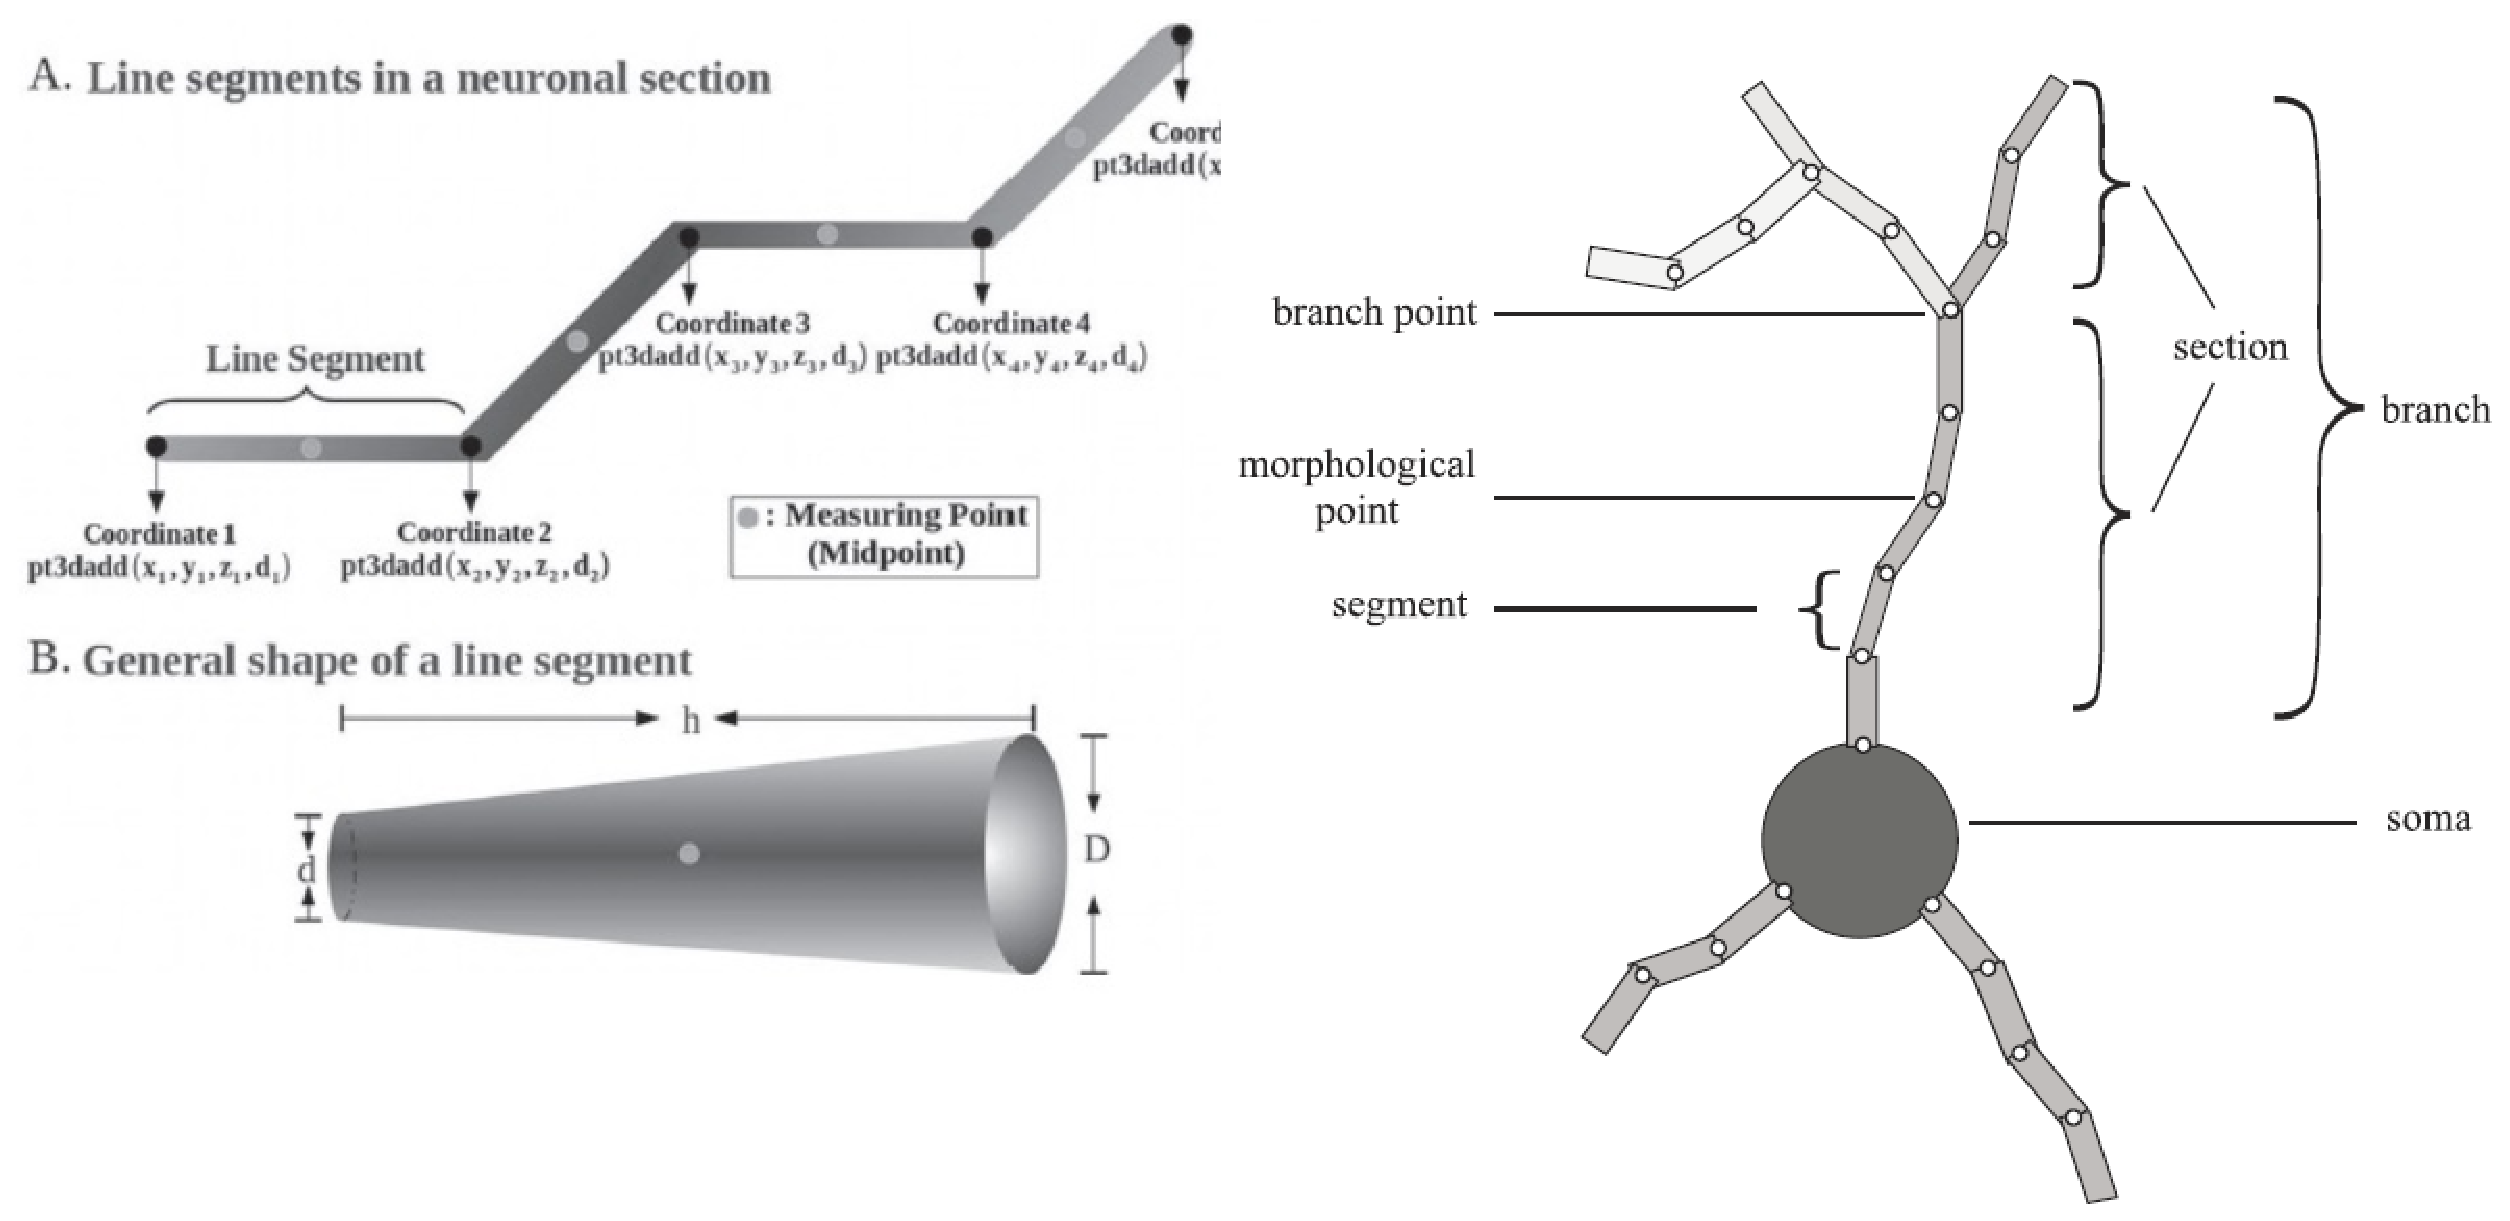
\includegraphics[height=5cm,
    angle=0]{./images/NEURON-3dpt-line-segment.eps}}
 \caption{3-D model: (A) line segments (Conical frusta
defined by two morphological points are called segments); (B) each line segment
is a truncated
 cone. 3D coordinates with an associated diameter are called morphological
 points. Based on Lasserre et al. (2012), a nonbranching sequence of segments
 defines a section; and the sequence of sections following the same path
 delineates a branch. Child sections are
sections that branch off of the parent sections at the branch point. Each branch
is connected to a parent branch or, in the case of first-order branches,
directly to the cell body of the neuron called soma
\citep{lasserre2012}}
\label{fig:NEURON-3dpt-line-segment}
\end{figure}


\begin{mdframed}
If the model is based on anatomical reconstruction data (quantitative
morphometry), or if 3-D visualization is paramount, it is best to use the 3-D
method.

\end{mdframed}

It is remapped to a straightened version of unit length,
Fig.\ref{fig:NEURON_section-segments}(C), and the underlying geometrical
morphology is separated from user's perspective.

\begin{figure}[hbt]
 \centerline{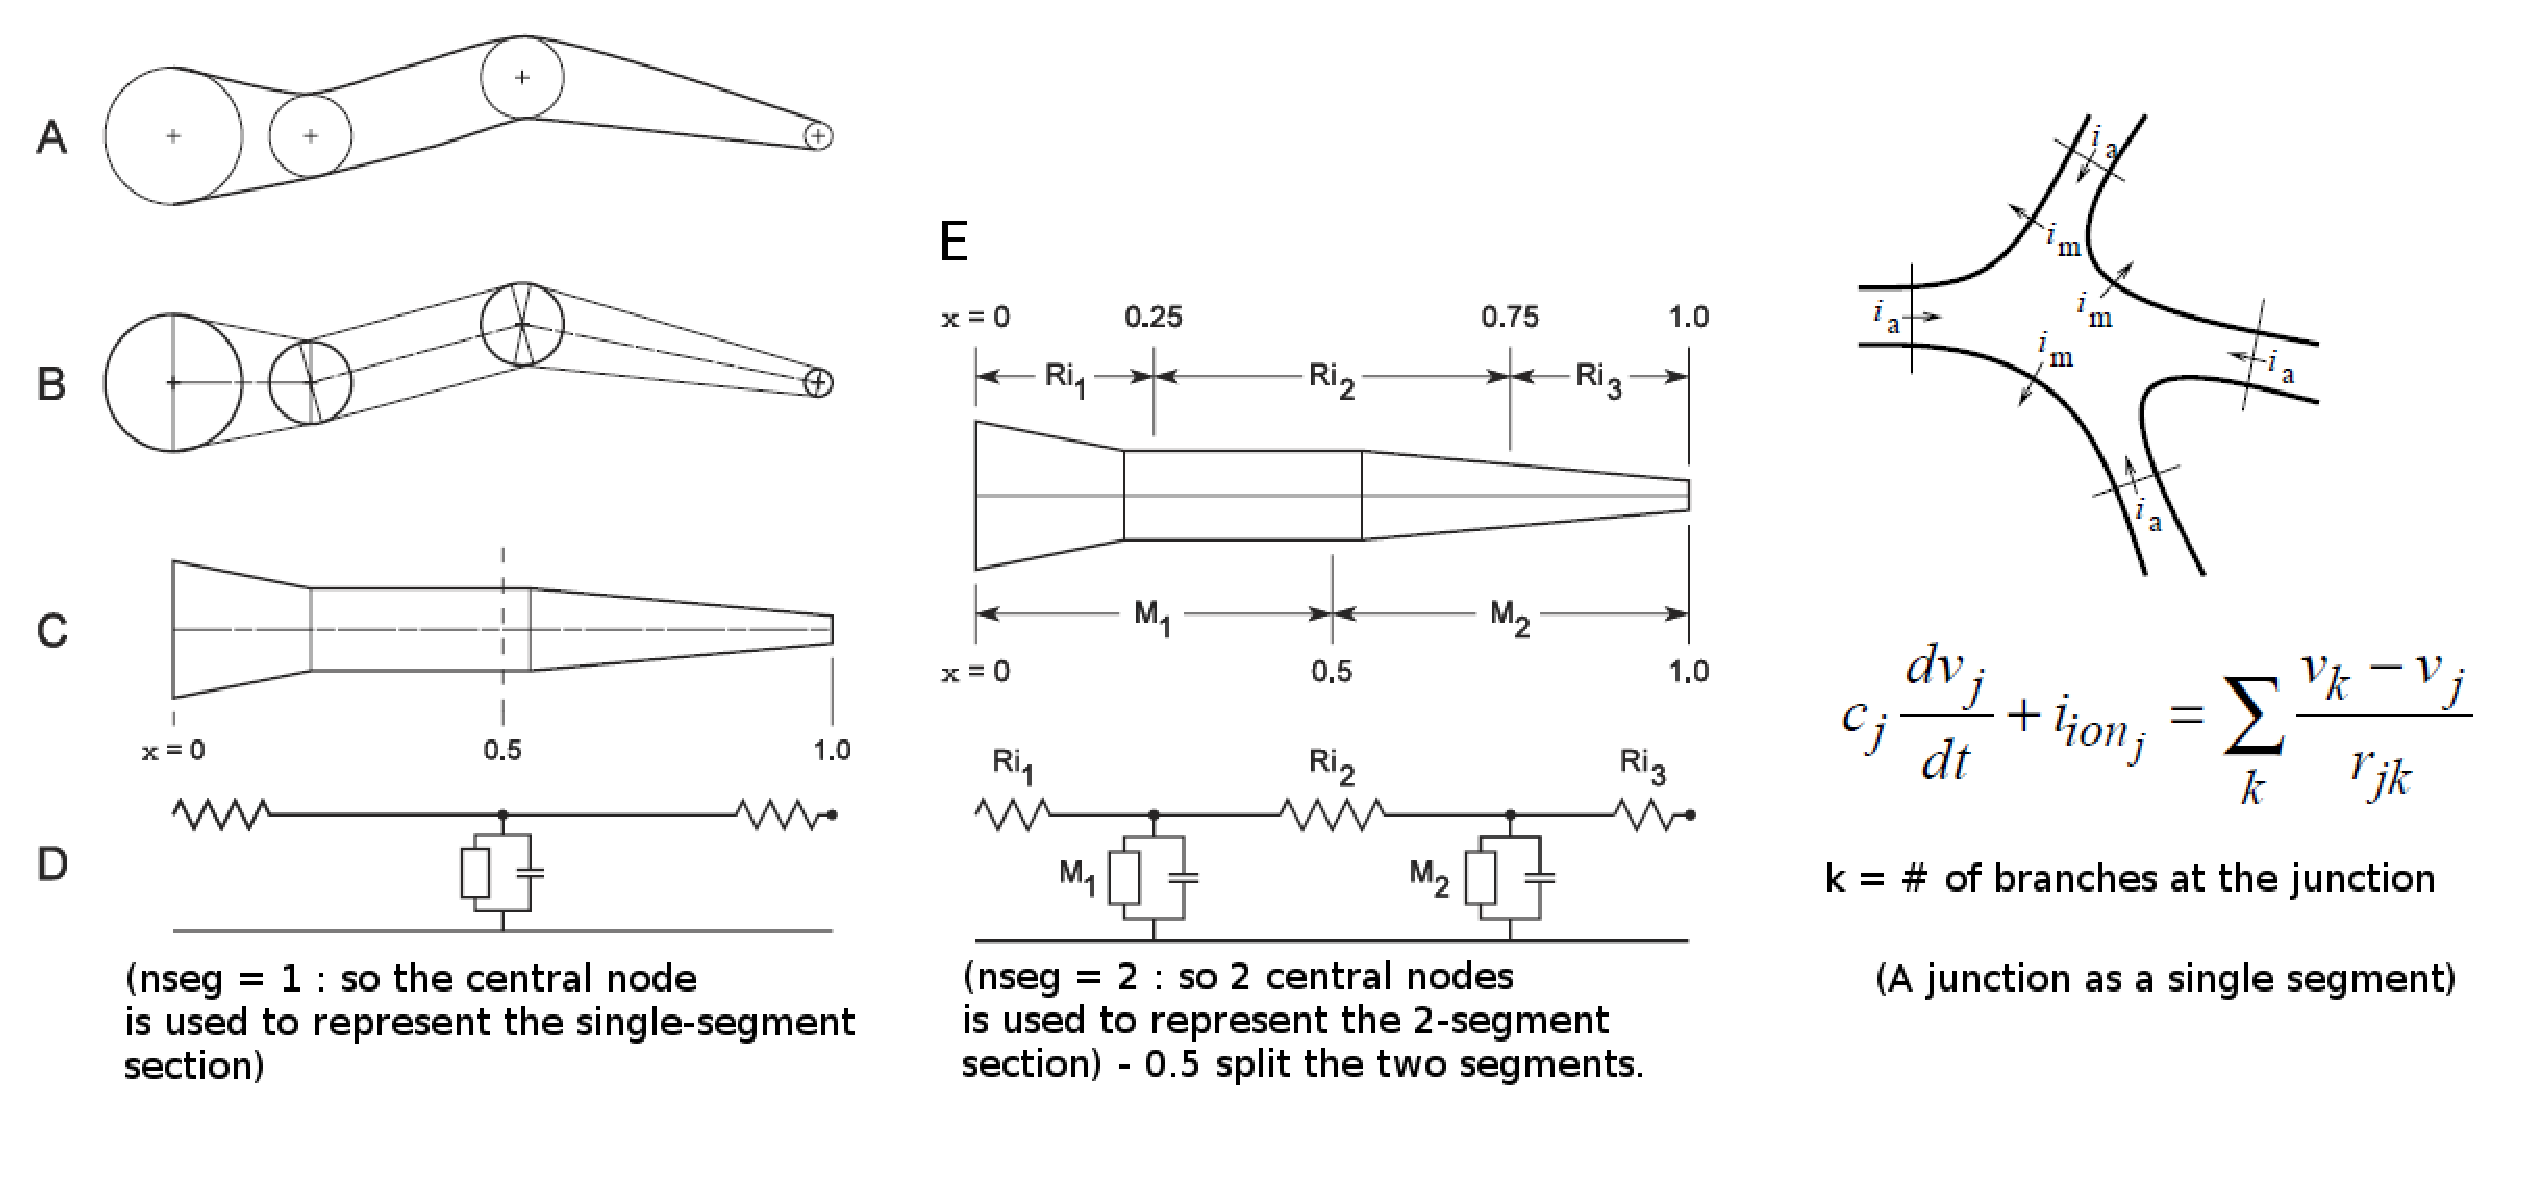
\includegraphics[height=6cm]{./images/NEURON_section-segments.eps}}
 \caption{(A) A neurite; (B) Every 2 points forms a capsule, a thin centerline
 pass through central axis of the chain of solids; (C) the centerline has been
 straightened }
\label{fig:NEURON_section-segments}
\end{figure}
 
The straightened version of the neurite is represented by a
{\bf section}, i.e. a continuous length of unbranched cable.
Each section is ultimately discretized into compartments (represented by
segments concept). To accommodate requirements for numerical accuracy, NEURON
represents each section by one or more {\bf segments} of equal length on that section.

The number of segments on that section is specified by the parameter
\verb!nseg!, which can be a different value for different sections.
\begin{itemize}
  \item nseg = 1: Fig.\ref{fig:NEURON_section-segments}(D)
  
The entire section is lumped into a single compartment.
This compartment has only one node, which is located midway along its length,
i.e. at x = 0.5.
\begin{enumerate}
  \item The integral of the surface area over the entire length of the section (0 
  $\le x \le 1$) is used to calculate the membrane properties associated with
  this node.

  \item The left and right hand axial resistances of
  Fig.\ref{fig:NEURON_section-segments}(D) are evaluated over the x intervals
  [0, 0.5] and [0.5, 1], respectively.
\end{enumerate}
  
  \item nseg = 2: Fig.\ref{fig:NEURON_section-segments}(E)
  
There are two segments of equal length that correspond to x intervals [0, 0.5]
and [0.5, 1].
\begin{enumerate}
  \item  The membrane properties over these
intervals are attached to the nodes at 0.25 and 0.75, respectively.
  
  \item The three axial resistors Ri1, Ri2 and Ri3
are determined by integrating the path resistance over the x intervals [0,
0.25], [0.25, 0.75], and [0.75, 1].
\end{enumerate}
  
\end{itemize}

\begin{itemize}
  \item At the center of each segment is a {\bf node}, the location where the
  internal voltage of the segment is defined.

The transmembrane currents over the entire surface area of a segment are
associated with its node. It is crucial to realize that the location of the
second order correct voltage is not at the edge of a segment but rather at its
center, i.e. at its node. This is the discretization method employed by NEURON

  \item To allow branching and injection of current at the precise ends of a
  section while maintaining second order correctness, extra voltage nodes that
  represent compartments with 0 area are defined at the section ends.

It is possible to achieve second order accuracy with sections whose end nodes
have nonzero area compartments. However, the areas of these terminal
compartments would have to be exactly half that of the internal compartments,
and extra complexity would be imposed on administration of channel density at
branch points.
  
  \item The nodes of adjacent segments are connected by resistors

  \item Based on the position of the nodes, NEURON calculates the values of internal
model parameters such as the average diameter, axial resistance, and compartment
area that are assigned to each segment.
    
\end{itemize}


Sections are connected together to form any kind of branched tree structure.
Each biologically significant component of a nerve cell has its counterpart in
one of the sections of the NEURON model
\begin{enumerate}
  \item cell body (Soma section)
  \item axon hillock (AH section) or axon initial section (AIS section)
  \item on the axons: 
  \begin{itemize}
    \item myelinated internodes: I$_i$ sections
    \item nodes of Ranvier: N$_i$ sections
  \end{itemize}
  
  \item dendrites: D$_i$ sections
\end{enumerate}



\subsection{numerical assumption}

Based upon the spatial descritization above, there are 2 important assumptions:
\begin{enumerate}
  \item  axial current is specified in terms of the voltage drop
between the centers of adjacent compartments, i.e. which is used to calculate
the distance.

  \item spatially varying
membrane current is represented by its value at the center of each compartment
\end{enumerate}

If the compartments are of equal size, it is easy to use Taylor's series to show that both of these
approximations have errors proportional to the square of compartment length.
Thus replacing the second
partial derivative (e.g. one-dimensional cable)
\begin{equation}
\frac{\partial V}{\partial t} + I(V,t) = \frac{\partial^2 V}{\partial x^2}
\end{equation}
by its central difference approximation (for a compartment $j$, and all its
$k$ adjacent compartments)
\begin{equation}
C_j \frac{dV_j}{dt} + I_{\ion,j}(V_j,t) = \sum_k \frac{V_k-V_j}{r_{jk}}
\end{equation}
introduces errors proportional to $\Delta x^2$, and
doubling the number of compartments reduces the error by a factor of four.

\textcolor{red}{Unequal compartment size (i.e. surface area) might be expected
to yield simulations that are only first order accurate}.
It is often not convenient for the size of all compartments to be equal.
However, comparison of simulations in
which unequal compartments are halved or quartered in size generally reveals a second-order reduction of
error. 
{\it A rough rule of thumb} is that simulation error is proportional to the
square of the size of the largest compartment.

\subsection{-- k=2 adjacent compartments}

\begin{equation}
C_j \frac{dV_j}{dt} + I_{\ion, j}(V_j,t) = \frac{V_{j-1} - V_j}{r_{j-1,j}} +
\frac{V_{j+1} - V_j}{r_{j,j+1}}
\end{equation}

The capacitance $C_j = \Csc \pi d \Delta x_j$ with $d=$ diameter of the
compartment, and $\Delta x_j$ = length of the compartment.

Axial resistance $r_{j-1,j} = R_a \frac{\Delta x{j-1,j}}{\pi (d_{j-1,j}/2)^2}$,
with $R_a$ = axial resistivity (which has different reported value for
different cell classes - Sect.\ref{sec:axial-resistivity}).

\subsection{-- k>2: junction point}


The branched architecture is incorporated by combining equations with
appropriate boundary conditions (i.e. statement of Kirchoff's current law)
\begin{verbatim}
sum(I_a) + sum(I_m) = 0
\end{verbatim}
The sum of all axial-current (into the junction as positive value) is equal in
magnitude, but in opposite sign, to the sum of all membrane currents (outward direction as
positive value).

Now, the transmembrane currents (outward direction as positive value) which
comprise capacitive current and all ionic currents)
\begin{equation}
\text{sum(I\_m)} = - C_j \frac{dV_j}{dt} - \sum( I_{\text{ion}})
\end{equation}
and the axial currents (into the junction $j$ as positive value)
\begin{equation}
\text{sum(I\_a)} = \sum_k \frac{V_k - V_j}{r_{jk}} + \text{I\_inj} 
\end{equation}
\url{https://neuron.yale.edu/neuron/static/papers/nc97/nc3p1.htm}

The capacitance $C_j = \Csc . \pi . d . \Delta x$, with assuming
the compartment $j$ has the length  dx and diameter d; and the axial resistance
\begin{equation*}
r_{jk} = R_a . \frac{dx}{pi (d/2)^2}
\end{equation*}.


This equation involves 2 approximations
\begin{enumerate}
  \item  axial current is specified in terms of the voltage drop between the
  centers of adjacent compartments 
  
  \item  spatially varying membrane current is represented by its value at the
  center of each compartment.
\end{enumerate}
This is much less drastic than the often heard statement that a compartment is
assumed to be "isopotential." It is far better to picture the approximation in
terms of voltage varying linearly between the centers of adjacent compartments.
Indeed, the linear variation in voltage is implicit in the usual description of
a cable in terms of discrete electrical equivalent circuits.

\textcolor{red}{What is the error in such 2 approximations?}
If the compartments are of equal size, it is easy to use Taylor's series to
show that both of these approximations have errors proportional to the square of
compartment length. Thus replacing the second partial derivative by its central
difference approximation introduces errors proportional to dx$^2$, and doubling
the number of compartments reduces the error by a factor of four.

NOTE: It is often not convenient for the size of all compartments to be
equal.Unequal compartment size might be expected to yield simulations that are
only first order accurate.  However, comparison of simulations in which unequal
compartments are halved or quartered in size generally reveals a second-order
reduction of error. 

NOTE: A rough rule of thumb is that simulation error is proportional to the
square of the size of the largest compartment.

\textcolor{red}{CASE 01} (an interior of an unbranched cable with constant
diameter): (internal node) compartment $j$ is between 2 other (internal nodes)
compartments.

\textcolor{red}{CASE 02} (the interior at each end of the unbranched cable): the
(internal node) compartment 1 (1-based index) and $(n)$: there are three
choices
\begin{enumerate}
  \item  where the right hand side consists only of the single term, 
  $\frac{v_{n-1} -v_n}{r_{n-1,n}}$ when compartment $(n)$ lies at the end of
  an unbranched cabl

  \item use the same formula, yet the internal node 1 and n-th, each need to
have an associated (terminal node) point. The terminal nodes have zero surface
areas, i.e. no membrane properties are associated with terminal nodes so the
voltage at the 0 and 1 locations is defined by a simple algebraic equation (the
weighted average of the potential at adjacent internal nodes) rather than an
ordinary differential equation.

It is possible to achieve second order accuracy with sections whose end nodes
have nonzero area compartments. However, the areas of these terminal
compartments would have to be exactly half that of the internal compartments,
and extra complexity would be imposed on administration of channel density at
branch points.

\end{enumerate}

Nerve boundary conditions are that no axial current flows at the end of the
cable, i.e. the end is sealed. 

\url{https://www.cell.com/biophysj/pdf/S0006-3495(75)85788-2.pdf}

\subsection{nrn}
\label{sec:nrn-NEURON}

{\bf nrn} is the binary name of the NEURON simulator (can be used for a cluster
of workstations or supercomputers). 

It uses its own scripting language: {\bf NMODL} - Sect.\ref{sec:NMODL} (based on
\verb!hoc! - a floating-point calculator with C-like syntax), that allows the
expression of kinetic models in terms of kinetic scheme or set of differential
or algebraic equations. Recently, Python scripting has been added as an
alternate to develop the model.

Before you can run the simulation, the code in HOC script need to be translated
into C, compiled, and linked into the rest of NEURON for simulation. A built-in
object-oriented interpreter can define morphology and membrane properties of
neurons, control the simulation, and display output in graphs.

The numerical method is described in
Sect.\ref{sec:model-dendrite-branching-Hines-algorithm}.

\subsection{section}
\label{sec:NEURON-section}
\label{sec:section-NEURON}

In NEURON, \verb!sections! are unbranched lengths of continuous cable. They are
conceptual represention of a neurite (Sect.\ref{sec:neurite}).
\begin{itemize}
  \item  Sections can be connected to form any tree-shaped structure but loops
  are not permitted. This is the basis for a neuron morphology.
  
  NOTE: you are allowed to develop membrane mechanisms, such as electrical gap
  junctions which do not have the loop restriction.
  
  
  \item  Sections are divided into segments of equal length for numerical
  simulation purposes (Sect.\ref{sec:Segment}).
  Such segments are similar to compartments in compartmental modeling programs.

  Section geometry is used to compute the area and axial resistance of each
  segment. This includes: L, nseg, diam, Ra, and connectivity.
  \begin{enumerate}
    \item L = length of the section
    \item nseg = number of segments in the section (to follow lambda rule -
    Sect.\ref{sec:lambda-rule-NEURON})
    \item diam = a range variable and must be respecified when nseg is changed
    
    \item Ra = axial resistivity (Ohm.cm)
    
    \item connectivity = the \verb!connect! command attaches the end of the
    section to the parent section; and where on the parent section the
    attachment take place
    
    NOTE: To avoid confusion, it is best to attach the 0 end of a section to the
    1 end of its parent.
  \end{enumerate}
  
\end{itemize}

\url{http://www.neuron.yale.edu/neuron/static/new_doc/modelspec/programmatic/topology/geometry.html}

\begin{verbatim}
          Ra
o/`--o--'\/\/`--o--'\/\/`--o--'\/\/`--o--'\o v
     |          |          |          |
    ---        ---        ---        ---
   |   |      |   |      |   |      |   |
    ---        ---        ---        ---
     |          |          |          |
-------------------------------------------- ground
\end{verbatim}



\subsection{* Example of a neuron model}

A model cell can have some sections specified by the stylized method
(Sect.\ref{sec:stylized-model-NEURON}), and others by the pt3d method
(Sect.\ref{sec:pt3d-method-NEURON}), but for any one section just be sure to
pick one style and stick with it.  Don't change from one to the other in the middle of specifying the geometry of a section and
expect the interpreter to guess what the dickens you intend.
\url{http://www.neuron.yale.edu/phpBB/viewtopic.php?f=15&t=2157}

\subsection{-- define components + connectivity}

\textcolor{red}{\bf Step 1.a } - create sections:

Before we set the section's properties, we must first create a new section,
soma, as follows, e.g. \verb!create soma!.
\begin{verbatim}
// create 5 sections, the 'dendrite' section has 3 instances
create soma, axon, dendrite[3]

\end{verbatim}


\textcolor{red}{\bf Step 1.b } - define connectivity:
 
\begin{verbatim}

// define the connectivity
// which we can use loop to connect multiple compartments
connect axon(0), soma(0)

  // here it is assumed all dendrite connect to soma
for i=0,2 { connect dendrite[i](0), soma(1)}

\end{verbatim}

NOMDL statements:
\begin{itemize}
 
  \item \verb!create! statement
  
  \item  \verb!connect! statement: to connect one section to another

%  \item  s

\end{itemize}

\subsection{-- (optional) define anatomical properties}

A section' default properties include (the number of segments in the section
[1], the diameter [500 $\mum$], the length [100 $\mum$], the specific membrane
capacitance [1 $\muF/\cm^2$] and the cytoplasmic resistivity [35.4 ohm cm]).

\textcolor{red}{\bf Step 2 } - we can change the default properties: define
anatomical (how many segments) and biophysical properties (conductance,
reversal potential).

{\it NEURON defines a number of predefined names}: diam, L, Ra, nseg. 

Here we use stylized model (Sect.\ref{sec:stylized-model-NEURON}), the diameter
of the section (\verb!diam!), the length of the section (\verb!L!), and the
axial resistance (\verb!Ra!), and the number of segments in the section
(\verb!nseg!) which also equal to the number of internal points (central nodes)
at which NEURON computes solutions. We can imagine that a section is broken into
nseg compartments of equal length (L/nseg), and that NEURON will compute the
time course of these variables at the centre of each compartment.

NOTE: In 3D model, the information about section length and diameter can be
computed directly from morphological data (with x,y,z, radius for each
end-point).

NOTE:If we assume that the density of transmembrane current is reasonably
uniform over the surface of the soma, a single point will be sufficient, and we
can assign a value of 1 to nseg.

\begin{verbatim}
soma { 
   nseg = 1
   L    = 50         // length (um)
   diam = 50         // diameter (um)
   insert hh          // standard HH current
   gnabar_hh = 0.5*0.120    // max HH Na+ conductance at soma
}


axon {
  nseg = 20
  L = 1000
  diam = 1
  insert hh
}


for i=0,2 dendrite[i] {
   nseg = 5
   L = 200
   diam(0:1) = 10:3  // dendritic diameter taper along its length
   insert pas      // standard passive current
   e_pas = -65       //reversal potential for passive current (mV)
   g_pas = 0.001     //conductance for passive current (Siemens/cm^2)

}
\end{verbatim}

To interact with a specific property, there are 3 ways
\begin{enumerate}
  \item \verb!dot! notation: section name followed by a dot or period (.)
  and then property name, e.g. \verb!stim.del! or \verb!soma.nseg=1!
  
  \item name of the section on the same line and immediately in front of a
  statement that refers to a section property:
  \verb!soma nseg = 1!
  
NOTE: group multiple properties within braces
\begin{verbatim}
soma {
    nseg = 1
    diam = 18.8
    L = 18.8
    Ra = 123.0
}
\end{verbatim}

NOTE: C programmers should note that the brace \verb!{! cannot be on its own
line.

  \item use \verb!access! statement to declare the default section
\begin{verbatim}
access soma

nseg = 1  // it refers to soma.nseg 
diam = 4.0
\end{verbatim}
\url{http://web.mit.edu/neuron_v7.3/nrntuthtml/tutorial/tutA.html}

\end{enumerate}

\subsection{-- define channels}

A natural first step in thinking about voltage-dependent or ligand-gated channel
models or elaborate cartoons of dynamic processes is to express them with chemical
reaction notation, i.e. kinetic schemes (Sect.\ref{sec:kinetic-scheme}).


\subsection{-- define pumps}

Example: $\Ca$-pump that pump $\Ca_i$ in a thin shell inside the membrane. The
dynamics of $[\Ca]_i$ is defined by 3 ODEs.
The active transport of calcium is represented by a pair of first order reactions
between calcium ions in solution on either side of cell

\begin{figure}[hbt]
 \centerline{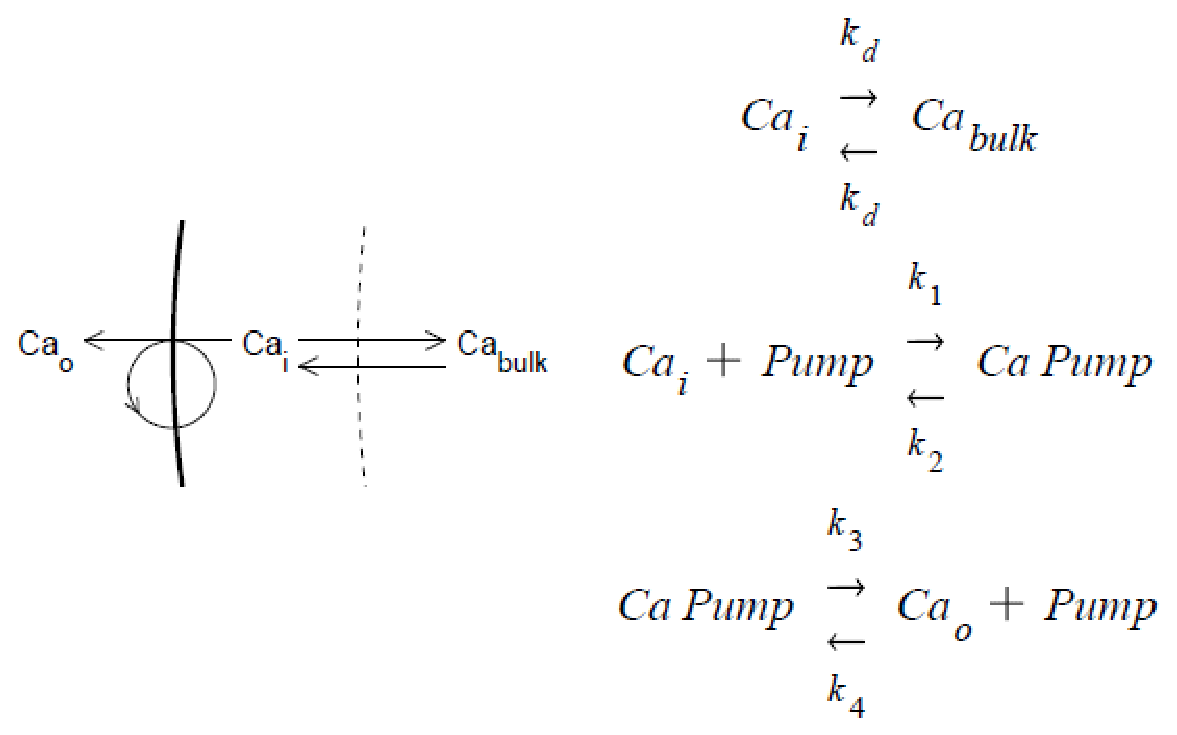
\includegraphics[height=10cm]{./images/Calcium-pump-scheme.eps}}
\caption{$\Ca$-pump: $\Ca_i$ in a thin shell inside the cell membrane is
regulated by (1) passive diffusion to the bulk in the core of the cell, and (2)
a pump in the cell membrane
}
\label{fig:Calcium-pump-scheme}
\end{figure}


The reactants occupy four regions, each of which has a different size. If the
volume of the core (vol-bulk) is much larger than that of the shell (vol-shell),
then a small amount of calcium could move from the core to the shell and have a
significant effect on the concentration Cai while there is almost no change in
the concentration Cabulk.

We start by defining the {\bf quantity of material} as the product of the state
variable and the size of its compartment (Sect.\ref{sec:kinetic-scheme}), and
then ensure that each term in the equation has the same units.

\subsection{-- define ion concentration (ca $\rightarrow$ ca\_ion)}

Example:
\begin{verbatim}
USEION ca READ ica WRITE cai, cao
\end{verbatim}

Each ion type is managed by its own separate ion mechanism (whose name is
created by adding \verb!_ion! suffix to the ion name specified in USEION
statement, e.g. becoming \verb!ca_ion!).
Here, the mechanism \verb!ca_ion! keeps track of
\begin{itemize}
  \item total current membrane carried by the ion, i.e. ica
  \item total intracellular concentration, i.e. cai
  \item total extracellular concentration, i.e. cao
  \item its equilibrium potential, i.e. \verb!eca!
\end{itemize}




\subsection{*** non-standard unit (no scale-factors)}
\begin{itemize}
  \item concentration (Cao, Cai, Cabulk): $\mu-mole/\cm^3$
  \item material densities (Pump and CaPump): $\mu-mole/\cm^2$
  \item area: [cm$^2$]
  \item volume: [cm$^3$]
\end{itemize}


\begin{verbatim}
vol_bulk * dCabulk/dt = k_d * Cai - k_d * Cabulk

vol_o * dCao/dt  = k_3 * CaPump - k_4 * Cao * Pump

vol_shell * dCai/dt = k_d * Cabulk - k-d * Cai
                     - k_1 * Cai * Pump + k_2 * CaPump
\end{verbatim}

Then, to ensure the same units on both side (which is $\mu-mole$/ms), the
units of the terms
\begin{itemize}
  \item $k_d$ : [cm$^3$/ms]
  \item $k_3$: [cm$^3$/ms]
  
  \item $k_4$: [cm$^5$/($\mu-mole$.ms)]
\end{itemize}

The third ODE
\begin{verbatim}
area_pump * dCaPump/dt = k_1 * Cai * Pump + k_4 * Cao * Pump
                        - (k_2 + k_3) * CaPump
\end{verbatim}
the unit of 
\begin{itemize}
  \item $k_1$: [cm$^5$/($\mu-mole$.ms)]
  \item $k_2$: [cm$^2$/ms]
\end{itemize}



\subsection{*** standard units (need scale-factors)}


\begin{itemize}
  \item concentration (Cao, Cai, Cabulk): $\mu-mole$/liter or $\muM$

NOTE: 1 $\mu$mole/cm$^3$ is equivalent to 1 millimole/liter, i.e. the values are
numerically equal, so {\bf we can use the same rate constants} and equations as
before, without having to insert scale factors into our equations.
  
  \item material densities (Pump and CaPump): $\mu-mole/\cm^2$
 
  \item area: [$\mum^2$]
  
  
  \item volume (volbulk, volshell): [$\mum^3$]

NOTE: $[\mum^3 \mu-mole/(ms. cm^3)]$ is equivalent to $10^{-12}$
[$\mu-mole/ms$].

\end{itemize}

In terms of volume, we need to scale a factor of $10^{12}$ on the right-hand
side

\begin{verbatim}
vol_bulk * dCabulk/dt = (k_d * Cai - k_d * Cabulk) * 10^12

vol_o * dCao/dt  = (k_3 * CaPump - k_4 * Cao * Pump ) * 10^12

vol_shell * dCai/dt = (k_d * Cabulk - k-d * Cai
                     - k_1 * Cai * Pump + k_2 * CaPump) * 10^12
\end{verbatim}



\subsection{-- define biophysical properties: insert channels into sections}


NOTE: other mechanisms (e.g., channels) with their own properties must
be explicitly inserted into a section using two built-in channel membrane
mechanisms: \verb!hh! (Hodgkin-Huxley channels) and \verb!pas! (passive
channels).

Script: 
\begin{enumerate}
  \item \verb!insert! statement assign a biophysical mechanism that govern
  electrical signal for each section.

\begin{verbatim}
insert hh
\end{verbatim}  

NOTE:
\begin{verbatim}
gnabar_hh: The maximum specific sodium channel conductance [Default value = 0.120 S/cm2]

gkbar_hh: The maximum specific potassium channel conductance [Default value = 0.036 S/cm2]

gl_hh: The maximum specific leakage conductance [Default value = 0.0003 S/cm2]

ena: The reversal potential for the sodium channel [Default value = 50 mV]

ek: The reversal potential for the potassium channel [Default value = -77 mV]

el_hh: The reversal potential for the leakage channel [Default value = -54.3 mV]
\end{verbatim}

\begin{verbatim}
soma insert pas
\end{verbatim}

  \item 
\end{enumerate}


\subsection{-- define stimulus}

\textcolor{red}{\bf Step 3} - define the stimulus which in this example is
modeled as a point process.

\begin{verbatim}
objref stim      // create a new stim object

soma stim = new IClamp(0.5)   // the object put onto 
    // the middle (0.5) of the soma 
    // as a current stimulus

stim.del   = 1      // delay (after the starting of simulation) (msec)
stim.dur   = 0.1    // duration of stimulus (msec)
stim.amp   = 60     // amplitude of stimulus (nA) - square-shaped only
\end{verbatim}

{\bf Density mechanism vs Point process}:
\begin{itemize}
  \item Many source of electrical and chemical signal are distributed over the
  membrane of the cell. They are modeled as {\bf density mechanisms}
  
  Unit: current per unit area, conductance per unit area
  
  \item Some quantities require using absolute value, e.g. current in
  nanoamperes, and conductance in Siemens to represent the signal at one
  particular location. They are modeled as {\bf point processes}.
  
  Example:
\begin{verbatim}
soma stim  = new IClamp(0.5)

dendrite[2] stim.loc(1)    // move the current stimulus to the distal end of the
                          // third dendrite
\end{verbatim}
\end{itemize}

\subsection{-- synapse}

Step 4 - define synapse + point process: 
\begin{enumerate}
  \item AlphaSynapse - follow alpha function (Sect.\ref{sec:alpha-function})

\url{http://fohs.bgu.ac.il/nia/nia2003/neurolab/help/alphasyn.htm}

  \item Exp2Syn
\end{enumerate}
%\subsection{* synapse + electrodes}

A synapse is an object with a pre- and a post-synaptic logical connection.

Iterate through each synapse (by return a reference to it via \verb!syn!) of a
certain synaptic type \verb!type! of an object referenced by \verb!layer1!
\begin{verbatim}
for layer1.synapses(syn, type) {
// statements that manipulate the object reference named "syn"
// (The iterator causes "syn" to refer, in turn,
// to each synapse of a certain type in the layer1 object)
}
\end{verbatim}

\subsection{* ODE + algebraic equation}

A set of differential and nonlinear simultaneous equations are written using an
expression syntax such as
\begin{verbatim}
x' = f(x, y, t)
~ g(x, y) = h(x, y)
\end{verbatim}
with \verb!~! tilde introduces an algebraic equation.

\subsection{numerical methods}
\label{sec:NEURON-solver}

We call \verb!fadvance()! to integrate all sections
(Sect.\ref{sec:NEURON-section}) over the interval \verb!dt!, then the value of $t$ is
incremented by \verb!dt!. 

\begin{enumerate}
  \item \verb!dt! is an internal variable representing the fundamental
  integration time step; and is used by \verb!fadvance()!

\verb!Dt! is an internal variable (a multiple of \verb!dt!)  
telling how often to update plotting.

  \item \verb!t! is an internal global variable which represent the current time
  
  \item  \verb!secondorder! is an internal global variable which tells the
  method to be used for integration
  \begin{verbatim}
  0   --> (default) fully implicit Backward Euler 
          very numerically stable; give steady state in 1 step with dt=1e10
          numerical error proportional to dt
          
  1   -->  Crank-Nicholson method 
          numerical error proportional to dt^2 (for small dt)
          CANNOT be used with voltage-clamp
          Ionic currents are first-order correct
          Channel conductances are second-order correct when plotted as t+dt/2
          
  2   -->  Crank-Nicholson with fix up so that ionic currents are now
           second-order when plotted as t-dt/2
           V(t)
           g(t+dt/2)
           I(t-dt/2)
  \end{verbatim}

NOTE: The simplest numerical method is forward Euler -
Sect.\ref{sec:forward-Euler}.

As given above, NEURON supports
\begin{enumerate}
  
  \item NEURON's default integration method is Backward Euler, a fixed step
  first order implicit scheme that produces good qualitative results with large
  time steps when extremely stiff ODEs and even algebraic equations are present
  in the system, e.g. models that involve voltage clamps -
  Sect.\ref{sec:backward-Euler}

  \item Crank-Nicholson: Sect.\ref{sec:Crank-Nicolson-method}
  
When the global parameter \verb!secondorder! is set to 2
(Sect.\ref{sec:Crank-Nicolson-Hines}), NEURON uses a variant of the
Crank-Nicholson method. This has local error proportional to $\Delta t^2$ and is
therefore particularly accurate for small time steps.

The special feature of the Crank-Nicholson variant is its use of a staggered
time step algorithm to avoid iteration of nonlinear equations
(Sect.\ref{sec:iteration-solving-nonlinear-equation}).
\begin{verbatim}
V(t+dt/2) is calculated

V(t+dt) = 2 * V(t+dt/2) - V(t)
\end{verbatim}

  \item CVODE: (adaptive time-step) - Sect.\ref{sec:CVODE}
  
\label{sec:CVODE}

CVODE handles any kind of model description involving DERIVATIVE or KINETIC
representations of gating states, ion accumulation/diffusion, or nonlinear
current-voltage relations. It does not work with models that involve
extracellular mechanisms, linear circuits, perfect voltage clamps, or capacitors
between nodes.
  
User does not specify the time-step, but instead specifies tolerance criteria
for local relative and absolute errors. The solver then adjusts \verb!dt! and
the local error order of the implicit difference approximation, from first order
up to $O(\Delta t^6)$, so that the local error for each state is less than the
sum of its relative and absolute error tolerances
(Sect.\ref{sec:truncation-error}).

NOTE: With CVODE, it solves the system in the form
\begin{verbatim}
dy/dt = f(y)
\end{verbatim}
which is not obtainable in the presence of extracellular voltage, or some other
stuffs like LinearMechanism.
At any rate, the issues are
\begin{enumerate}
  \item how to compute f(y) 
  
Any algebraic equations are solved inside f(y) so that the algebraic states are
consistent with y.

  \item how to setup Jacobian 
  
\begin{verbatim}
(I - gamma * df/dy) * y = b
\end{verbatim}
\end{enumerate}

  
  \item DASPK method (Brown, Hindmarsh, and Petzold, 1994)

The DASPK method is suitable for models that involve extracellular mechanisms,
linear circuits, perfect voltage clamps, or capacitors between nodes. However,
there is no local variable step variant of DASPK.

DASPK solves the system in the form
\begin{verbatim}
f(y,y') = 0
\end{verbatim}
And the issue with DASPK are
\begin{enumerate}
  \item how to actually implement a residual function 
\begin{verbatim}
res = f(y, y')
\end{verbatim}

  \item how to actually implement preconditioned setup of the form

\begin{verbatim}
(df/dy + cj * df/dy') * y = b
\end{verbatim}

  \item how to initialize so that
  
\begin{verbatim}
f(y(0), y'(0)) = 0
\end{verbatim}
when it's not possibel to know which are algebraic equations and which are
differential equations.

NOTE: it is often the case that a linear combination of differential equations
yields an algebraic equation; and we don't know the linear combination subsets.

DASPK itself can handle initialization if user tells/marks which states are
differential; and the remaining states are algebraic.
\end{enumerate}

\end{enumerate}

\end{enumerate}

\subsection{-- order of solver}
\label{sec:run-NEURON}

WHOLE SIMULATION:  
\begin{verbatim}
run():
    init():
           finitialize(some-init-voltage)
    continuerun() or steprun()
           step():
                advance():
                        pre-loop-statement() - optional
                        fadvance()
                        post-loop-statement() - optional
\end{verbatim}

INIT PHASES:
\begin{enumerate}
  
  \item \verb!finitialize()! or \verb!finitialize(v_init)! -
  Sect.\ref{sec:finitialize-NEURON}
  
\begin{verbatim}
finitialize()
finitialize(v)
\end{verbatim}

\url{http://www.neuron.yale.edu/neuron/static/new_doc/simctrl/programmatic.html#finitialize}

\end{enumerate}

RUNTIME PHASES:
\begin{enumerate}
  \item \verb!fadvance()! call all BREAKPOINT block of every mechanisms to
  integrate all section equations over the time interval dt. After this, the
  time is increment by dt.
  
Default method is first-order implicit; but can be changed to -
Sect.\ref{sec:fadvance-NEURON}
\begin{verbatim}
fadvance(seconorder=2)
\end{verbatim}
  
   \verb!BREAKPOINT {SOLVE ... METHOD after_cvode}!
  
\begin{verbatim}
proc after_step()
\end{verbatim}
called at every fadvance() when t = t+dt. - Sect.\ref{sec:fadvance-NEURON}
  
  \item  The SOLVE statement is executed after the new voltages have been
  computed in order to integrate the states over the time step, dt. 
\end{enumerate}

\subsection{-- finitialize()}
\label{sec:finitialize-NEURON}
\label{sec:initmodel()-NEURON}
\label{sec:nrn_init()-NEURON}


\begin{verbatim}
init():
   finitialize() or finitialize(some-initial-voltage):  //v_init
      nrn_init(): 
         initmodel() for all models
\end{verbatim}

\verb!finitialize([vinit])! has an optional argument vinit; the function call
INITIALIZE block for all mechanisms in all segments (NOTE:  each mechanism is
defined in each NMODL file - Sect.\ref{sec:NMODL}). NOTE: Default initialization
sets all states (e.g. gating variables) to \verb!state0!.

ORDER:
\begin{enumerate}
  \item $t \leftarrow 0$ and event queue is cleared (undelivered events from the
previous run are thrown away).

  \item Variables that receive a random stream (the list defined by Random.
play() statements) are set to values picked from the appropriate
random distributions

  \item internal structures that depend on topology and geometry that depends on
  geometry and topology are updated
  
  \item controller for Vector.play() variables is initialized; with 
  events at time t=0 are
delivered.

  \item  If the optional argument is present then all voltages of all sections are
initialized to v (at time t=0).
\begin{verbatim}
// hoc code
forall for (x) v(x) = v_init
\end{verbatim}
  
  \item The INITIAL block of every inserted mechanism in every segment of
every section is called.

This includes point processes as well as
distributed mechanisms. The order
in which mechanisms are initialized depends on whether any
mechanism has a USEION statement or WRITEs an ion concentration
\begin{itemize}
  \item IMPORTANT:
  
if the INITIAL block of one mechanism needs the values of variable from another
mechanism, the latter should be assigned before finitialize() is executed.

  \item If extracellular mechanisms exist, their vext states are initialized to 0
before any other mechanism is initialized

  \item if it has USEION statement; the mechanisms are initiated first
  
  then mechanisms that WRITE an ion concentration are initialized
  
  \item if it has WRITEs an ion concentration:
  
  this necessitates recalculation of the equilibrium potentials for any affected
  ions, e.g. ena. 

  \item finally, all other mechanism INITIAL blocks are called.
  
  \item of user-defined mechanism (i.e. *.mod file):
  
  call order of user-defined mechanisms is currently defined by the alphabetic
  list of mod file names or the order of the mod file arguments to nrnivmodl (or
  mknrndll).

  \item 
\end{itemize}

   \item LinearMechanism states
   
   \item Network connections are initialized
   
   
the INITIAL block inside any \verb!NET_RECEIVE! block that is a target of a
NetCon object is called to initialize the states of the NetCon object.

    \item The INITIAL blocks may have initiated \verb!net_send! events whose
delay is 0. These events are delivered to the corresponding \verb!NET_RECEIVE!
blocks.

  \item If fixed step integration is being used: 
  all mechanism BREAKPOINT
blocks are called, i.e. fcurrent - sect.\ref{sec:fcurrent-NEURON}

In order to initialize all assigned variables (conductances and currents)
based on the initial STATE and membrane voltage.

  \item If any variable time step method is active, then those integrators are
  initialized.
  
\end{enumerate}




NOTE: user can also set things up in a model's INITIAL block
(Sect.\ref{sec:NMODL-block-INITIAL}) which can make use of voltage \verb!v!.
NOTE: With care, they can make use of ionic concentrations just like BREAKPOINT
and SOLVE blocks.

Example: nocmodl test.mod
\begin{verbatim}
/***************************/
static nrn_init(_count, _nodes, _data, _pdata, _type_ignore)
  int _count, _type_ignore; Node** _nodes; double** _data;
  Datum** _pdata;
{ 
int _ix; double _v;
_p = _data; _ppvar = _pdata;
#if _CRAY
#pragma _CRI ivdep
#endif

for (_ix = 0;_ix <_count; ++_ix){
  _v = _nodes[_ix]->_v;
  v = _v;
  ena = _ion_ena;
  initmodel(_ix);
}
}
/***************************/
\end{verbatim}

\subsection{---- initialize (of voltage, gate, ion concentration)}

\textcolor{red}{In the case of voltage}: finitialize(-65) will indeed set the
voltage to -65mV, and m, h, and n will be in steady state relative to that
voltage. Read Sect.\ref{sec:resting-membrane-potential-numerics} to learn how to
ensure that is the exact resting membrane potential.



\textcolor{red}{In the case of gates (m, n, h)}:
A default initialization of the STATEs of the model occurs just prior to the
execution of the INITIAL block. However, this default initialization is rarely
useful, and one should always explicitly implement an INITIAL block.

If the name of a STATE variable is state, then there is also
an implicitly declared parameter called state0.
If a specific value for state0 is not declared by the user (using 1 of the two
methods below), state0 will be assigned a default value of 0.


The default value of state0
is specified either in the PARAMETER block
\begin{verbatim}
PARAMETER {
state0 = 1
}
\end{verbatim}
or implicitly in the STATE declaration with the syntax
\begin{verbatim}
STATE {
state START 1
}
\end{verbatim}

{\bf IMPORTANT}: state0 is not accessible from the interpreter unless it is
explicitly mentioned in the GLOBAL or RANGE list of the NEURON block.
\begin{verbatim}
NEURON {
GLOBAL m0
RANGE h0
}
\end{verbatim}
every m will be set to the single global m0 value during initialization,
while h will be set to the possibly spatially varying h0 values. An explicit way
to do the same thing
\begin{verbatim}
INITIAL {
m = m0
h = h0
n = n0
}
\end{verbatim}

\textcolor{red}{\bf In the case of ion}:
The initial values of cai and and cao are set globally to the values of 
\verb!cai0_ca_ion!; and \verb!cao0_ca_ion!, respectively. 
The value of \verb!eca! is set by the \verb!ca_ion! mechanism as well. And thus
cannot be assigned through the model description in MOD file.

\begin{itemize}

   \item this is wrong practice in NEURON:
     
Example:  when a model declares an ion variable, such as ena (then the real
memory reference is name \verb!_ion_ena!), to be a PARAMETER and attempts to
assign a value to it in the PARAMETER block
  
\begin{verbatim}
NEURON {
SUFFIX test
USEION na READ ena
}
PARAMETER { 
// ena name here is a local copy; (whose value is assigned from
//  the global variable _ion_ena each time finitialize() is called 
//  doing this has no effect on ena

ena = 25 (mV)
}
\end{verbatim}
Compiler warning
\begin{verbatim}
Warning: Default 25 of PARAMETER ena will be ignored and
set by NEURON.
\end{verbatim} 

The model description (via using PARAMETER block) can touch only the local copy
and is unable to change the value referenced by \verb!_ion_ena!
(Sect.\ref{sec:nrn_init()-NEURON}).
  
  \item NEURON prior to 4.1: initialization is cumbersome
  
  It uses the ionic concentration adjacent to the membrane according to global
  variables.
  
  The reason that model mechanisms were not allowed to specify ion variables (or
  other potentially shared variables such as celsius) was that confusion could
  result if more than one mechanism at the same location tried to assign
  different values to the same variable.
  

 
NOTE RECOMMENDED HACK: Some old model descriptions circumvented this hiding by
using the actual reference to the ion mechanism variables in the INITIAL block
(from a knowledge of the translation implementation), but that was always
considered an absolutely last resort.
  
  
  \item Initialize (cai, cao, eca)	using WRITE statement; in the condition that 
  concentration is declared to be a STATE and the concentration is initialized
  explicitly in an INITIAL block
  
\begin{verbatim}
NEURON {
SUFFIX test2
USEION na WRITE nai
RANGE nai0
}

STATE {
nai (milli/liter)
}

INITIAL {
nai = nai0
}

PARAMETER {
nai0 = 20 (milli/liter)
}
\end{verbatim} 

LIMITS: Such a mechanism has an associated global variable that can be used to
initialize the concentration to the same value in each section where the
mechanism exists.

   \item Initialize using hoc code directly.

Example: the mechanism kext that implements extracellular potassium accumulation
as described by Frankenhaeuser and Hodgkin (1956). The kext mechanism
WRITEs ko, so the corresponding global variable is \verb!ko0_k_ion! for initial
value.
   
\begin{verbatim}
ko0_k_ion = 10 // seawater, 4 x default value (2.5)
ki0_k_ion = 4*54.4 // 4 x default value, preserves ek
finitialize(v_init) // v_init is the starting Vm
\end{verbatim}
will set ko to 10 mM and ki to 217.6 mM in every segment that has the kext
mechanism.

   
   \item NOW: whether the concentration is supposed to start at the same value
   in all sections where the mechanism has been inserted, or should it be
   nonuniform from the outset?

NEURON provides \verb!ion_style()! function

Example: in the dend section
\begin{verbatim}
dend ion_style("k_ion",3,2,1,1,0)

// or
ko0_k_ion = 10 // all sections start with ko = 10 mM
dend {ko = 5 ki = 2*54.4} // . . . except dend
finitialize(v_init)
\end{verbatim}

treat ko as a STATE variable; treat ek as an ASSIGNED variable;
on call to finitialize() use the Nernst equation to compute ek from
the concentrations; compute ek from the concentrations on every call to
fadvance().


\end{itemize}

\subsection{---------- save the state (oscilation system)}

This is useful, continue the simulation by using input data from the end of some
run is to serve as the initial condition for subsequent runs; this is a
particularly useful strategy for dealing with models that oscillate or otherwise
lack a "resting" state.

\begin{verbatim}
objref svstate, f
svstate = new SaveState()
svstate.save()


f = new File("states.dat")
svstate.fwrite(f)


\end{verbatim}

Future simulation, reread the last state
\begin{verbatim}
objref svstate, f
svstate = new SaveState()
f = new File("states.dat")
svstate.fread(f)

proc init() {
finitialize(v_init)
svstate.restore()
t = 0 // t is one of the "states"
if (cvode.active()) {
cvode.re_init()
} else {
fcurrent()
}
frecord_init()
}
\end{verbatim}

\subsection{--------- steady-state: find Vrest}
\label{sec:resting-membrane-potential-numerics-find}

NOTE: the backward Euler method can find the steady state of a linear system in
a single step if the integration step size is large compared to the longest
system time constant. Backward Euler can also find the steady state of many
nonlinear systems, but it may be necessary to perform several iterations with
large dt.


In NEURON, 
\begin{enumerate}
  \item set the starting time to very negative so that no event is generated.
  \item set very large time step to find steady-state after only 1 iteration,
  i.e. one fadvance().
  
  \item returning dt to its original value, setting t back to 0, and, if
  necessary, reactivating the variable step integrator 
\end{enumerate}
This initialization strategy generally works well, but there are circumstances in
which it may fail: Active transport mechanisms can be troublesome with fixed
time step integration if dt is large, because even a small pump rate may produce
a negative concentration. This underscores the need for careful testing of any
initialization strategy.

Code example:
\begin{verbatim}
proc init() { local dtsav, temp
finitialize(v_init)
t = -1e10
dtsav = dt
dt = 1e9
// if cvode is on, turn it off to do large fixed step
temp = cvode.active()
if (temp! = 0) { cvode.active(0) }
while (t<-1e9) {
fadvance()
}
// restore cvode if necessary
if (temp! = 0) { cvode.active(1) }
dt = dtsav
t = 0
if (cvode.active()) {
cvode.re_init()
} else {
fcurrent()
}
frecord_init()
}
\end{verbatim}


\subsection{--------- steady-state: enforce Vrest}
\label{sec:resting-membrane-potential-numerics}

NOTE: finitialize(-65) will indeed set the voltage to -65mV, and m, h, and n
will be in steady state relative to that voltage. 

HOWEVER: In a scenario of voltage clamp initialization, when trying to set -65mV
as the voltage-clamp, this may not be the resting potential. For this reason it
is common to adjust the equilibrium potential of the leak current so that the
resting potential is precisely -65mV.


\textcolor{red}{IMPORTANT}: After applying the strategy below, testing is
required to verify that the system is stable at the desired \verb!v_init! (i.e.
that the system returns to \verb!v_init! after small perturbations).

\begin{itemize}
  \item  a user-defined
init() procedure based on the idea that total
membrane current at steady state must be 0. 

\begin{verbatim}
0 = ina + ik + gl_hh*(v - el_hh)
\end{verbatim}
and recalculate \verb!el_hh! 
 
Example:
\begin{verbatim}
proc init() {
  finitialize(-65)
  
  el_hh = (ina + ik + gl_hh*v)/gl_hh

  if (cvode.active()) {
     cvode.re_init()  // implicit call to fcurrent() as well
  } else {
     fcurrent()
  }
  frecord_init()
}
\end{verbatim}

NOTE: \verb!cvode.re_init()! update the calculation of all the
dstate/dt (note that now dv/dt should be 0 as a consequence of the change in
\verb!el_hh!) as well as internally make a call to fcurrent() (necessary because
changing \verb!el_hh! requires recalculation of \verb!il_hh!).

WARNING: this approach is not fail-safe in the sense that the resultant value of
\verb!el_hh! may be very large and out of its physiological range, as
\verb!gl_hh! may be a very small quantity.
 
 
    \item better to introduce a constant current mechanism and set its value so
    that 
    
\begin{verbatim}
0 = ina + ik + ica + i_constant
\end{verbatim}
holds at the desired resting potential.

\begin{verbatim}
:constant current for custom initialization
NEURON {
SUFFIX constant
NONSPECIFIC_CURRENT i
RANGE i, ic
}
UNITS {
(mA) = (milliamp)
}
PARAMETER {
ic = 0 (mA/cm2)
}
ASSIGNED {
i (mA/cm2)
}
BREAKPOINT {
i = ic
}
\end{verbatim}

Example: user-defined init()
\begin{verbatim}
proc init() {
finitialize(-65)  // already
ic_constant = -(ina + ik + il_hh)

if (cvode.active()) {
cvode.re_init()
} else {
fcurrent()
}
frecord_init()
}
\end{verbatim}

\end{itemize}


\subsection{-- fadvance()}
\label{sec:fadvance-NEURON}

\textcolor{red}{\bf HOW IT WORKS} via \verb!run()! function
(Sect.\ref{sec:run-NEURON}).

\textcolor{red}{fadvance()}: the timing loop call \verb!fadvance()! as the main
function to update the system at each time step.
  
\begin{itemize}
  
  \item Assuming the entry time is \verb!tentry!. Then the input to
  \verb!fadvance()! is data
\begin{verbatim}
V(tentry)
gates (tentry+dt/2)
\end{verbatim}
%   assume at entry of \verb!fadvance()!
  \begin{enumerate}
    \item calculate discrete events : those occurs within the time
   \verb!tentry-dt/2! to \verb!tentry+dt/2!.
   
\begin{verbatim}
NetCvode::deliver_net_events()
\end{verbatim} 

     \item calculate the value of the variables (e.g. voltage command) if it is
     used to overwrite the variable; and the value needs to be interpolated to
     give the value estimated at time \verb!tentry+dt/2!

\begin{verbatim}
Vector.play(&var, vec, tvec)
\end{verbatim}     

\textcolor{red}{Change since NEURON 5.4}: \verb!Vector! that are played onto a
variable (e.g. v) is now considered as a sequence of discrete events (part of
step 1). 

     \item update the system using matrix M (whose elements are data calculated
     at time \verb!tentry+dt/2!: this needs multiple steps
   
 \begin{verbatim}
 //fixed time-step
 void *setup_tree_matrix(NrnThread *_nt) {
  nrn_rhs(_nt);
  nrn_lhs(_nt);
  nrn_nonvint_block_current(_nt->end, _nt->_actual_rhs, _nt->id);
  nrn_nonvint_block_conductance(_nt->end, _nt->_actual_d, _nt->id);
  return (void *)0;
}
 \end{verbatim}  
 
     setup elements for matrix M
     \begin{equation}
     \mathbf{M}. \mathbf{v} = \mathbf{r.h.s}
     \end{equation}
     with {\bf M} is a diagonal matrix (representing an unbranched cable/tree)
     with \verb!a! (above), \verb!b! (below), \verb!d! (diagonal) elements.
     
     NOTE: \verb!d! are conductance density unit; \verb!r.h.s.! are current
     densities units.
     
     \begin{itemize}
       \item check flag: to see if the geometry change, then update \verb!Aij!
       and \verb!Aip! values (in the matrix M in NTS) or \verb!Node[i].a! and
       \verb!Node[i].b! values (in the matrix M in NEURON) 
       
 Setting up 'a' and 'b' is given by \verb!method3_connection_coef()! in metho3.c
 file. 
       
       \item reset \verb!d! and \verb!r.h.s.! values for matrix M to zero.
   
       \item update mechanisms, i.e. execute BREAKPOINT blocks of all mechanisms
       - Sect.\ref{sec:BREAKPOINT-block-NEURON}
 
 {\small      
\begin{verbatim}
C * delta_V_j / delta_t - sum_k (delta_V_k - delta_V_j) / [ area_k * r_{jk}]
    = -iion (V_j(t+dt)) +  sum_k (V_k - V_j) / [ area_k * r_{jk}]  + I_stim
\end{verbatim}
}

One way to approximate \verb!iion(V_j(t+dt)! is
\begin{verbatim}
iion (V_j(t+dt)) = iion(V(t)) + delta_V_i * di/dv
\end{verbatim}

The effects of membrane conductance changes on model dynamics are taken into
account by executing statements in the BREAKPOINT block twice--once with an
argument of v+0.001 and again with an argument of v--in order to calculate a
numerical estimate of the derivative di/dv.
This conductance is added to the corresponding diagonal element of the Jacobian
matrix that had been set up during initialization. This means that if a density
mechanism or point process generates a current, the statement in which that
current is calculated should be executed in the BREAKPOINT block.  

       
       \item update \verb!d! and \verb!r.h.s.! values for matrix M

    If backward Euler method is used to update V(t) to V(t+dt)
       \begin{enumerate}
         \item add \verb!di/dv! to \verb!d! (Node.d)
         \item add \verb!-i (t)!  to \verb!r.h.s!   
       \end{enumerate}

{\small
\begin{verbatim}
C * delta_V_j / delta_t - sum_k (delta_V_k - delta_V_j) / [ area_k * r_{jk}]
   + delta_V_j * di/dv
    = -iion (V_j(t)) +  sum_k (V_k - V_j) / [ area_k * r_{jk}]  + I_stim
\end{verbatim}
}

\verb!nrn_solve()! solve the voltage-node equations. On return,
\verb!nrn_solve()! set the \verb!r.h.s.! field of the node as the value of
$\Delta V$ (from v(t) to v(t+dt)). NOTE: Voltage still has not been updated yet.

       \item {\bf ionic currents}:
       
    If Crank-Nicholson secondorder=2 is used (then remember V(t), gate(t+dt/2))
    \begin{verbatim}
    then the currents (e.g. GHK current) are updated with a call
to second_order_cur(), which uses di_ion/dv along with
delta_v to compute the second-order correct
ionic currents at tentry+dt/2

Note that individual currents associated with particular
channel mechanisms and available to the
interpreter as ASSIGNED variables are not
updated to be second order correct, i.e. individual model description current
variables are only approximated by 
   iion(texit - dt/2) = g(texit + dt/2) * (v(texit-dt) - erev).
   
Correcting this variable requires another evaluation   
    \end{verbatim}    
       
Example: ASSIGNED block - Sect.\ref{sec:ASSIGNED-block-NEURON}       
       
       
       \item {\bf update voltage}:
       
 If backward Euler, then $\Delta V$ (or r.h.s.) hold the increment from v(t) to
 v(t+dt); so update 
 
 \begin{verbatim}
 v(t+dt) <-------- v(t) + r.h.s.
 \end{verbatim}

 If Crank-Nicholson is used, then $\Delta V$ (or r.h.s.) hold the
 increment from v(t) to v(t+dt/2); so update 
 
 \begin{verbatim}
 v(t+dt) <-------- v(t) + 2 * r.h.s.
 \end{verbatim}

\textcolor{red}{Now t is incremented to tentry+dt}.

      \item {\bf nonvinit()}: integrates all states EXCEPT voltages (this is
      done when no \verb!v_init! is passed in.

%\ref{sec:fcurrent-NEURON}
       
      \end{itemize}
  \end{enumerate} 
  
  
%   \item call all the BREAKPOINT blocks of models at (t+dt/2) twice; 
%   with v+.001; and \verb!v! 
%   
%   to compute the current and conductance to form the matrix:
%   conductance*voltage=current.
   
  
  \item the matrix is solved for v(t+dt/2)

\begin{verbatim}
v = v + r.h.s //backward Euler

v = v + 2 * r.h.s // Crank-Nicholson secondorder=2
\end{verbatim}  
%v(tentry+dt) = 2 * v(tentry+dt/2) - v(tentry)

 NOTE: Here an additional step is used to adjust the ionic currents to be
 second-order if \verb!secondorder=2!. 
 
  \item the SOLVE statement within the BREAKPOINT block of models is executed
  with t+dt and the new values of \verb!v! 
  
  to integrate those states from new (t-dt/2) to (t+dt/2).
   
\end{itemize}

\subsection{-- fcurrent}
\label{sec:fcurrent-NEURON}

fcurrent() function contains the code to make the values of all conductances and
currents consistent with the newly initialized states.
Each BREAKPOINT (in a single mechanism) is mapped to this function.

fcurrent is used to set up all assigned variables  without changing any
states.  It assumes all states have their values at time t which is
only first order correct. It determines the nonvint assignments first
so that ena, etc. are correct for the current determinations. We
demand that nonvint assignments can be done without changing states when
dt is temporarily set to 0. It turns out to be a bad idea to do this.


In particular this will call the BREAKPOINT block (twice, in order to compute
the Jacobian (di/dv) elements for the voltage matrix equation) for all
mechanisms in all segments, and on return the ionic currents such as ina, ik,
and ica will equal the corresponding net ionic currents through each segment.

For several integration methods (e.g. backward Euler), BREAKPOINT assignment
statements are often executed twice to calculate the di/dv terms of the Jacobian
matrix.

For Crank-Nicholson (secondorder=2), then given v(t), gate(t+dt/2)
\begin{verbatim}
dV = v(t+dt/2) - v(t)

iion (v(t+dt/2)) = iion(v(t)) + dV * di/dv
\end{verbatim}

NOTE: 
\begin{verbatim}
di/dv = i(v(t)+0.001) - i(v(t)) / 0.001
\end{verbatim}


\subsection{ghk() - Goldman-Hodgkin-Katz current}

The function in NOMDL 
\begin{verbatim}
ghk(v, ci, co, charge)
\end{verbatim}
returns GHK current (normlized to unit permeability) -
Sect.\ref{sec:Nernst-Planck-equation}, Sect.\ref{sec:GHK_current}.


In NEURON,
\begin{verbatim}
mA/cm^2 = (permeability in cm/s) * ghk(mV, mM, mM, valence)
\end{verbatim}


In order to use this, the model should include calcium intracellular and
extracellular concentration accumulation mechanism, i.e. a mechansim with
\verb!USEION!
\begin{verbatim}
USEION calcium READ ci, co WRITE ica
\end{verbatim}

Example: Potassium leak code following GHK
{
\begin{verbatim}
: kghk.mod
: potassium leak governed by Goldman-Hodgkin-Katz equation

NEURON {
  SUFFIX kghk
  USEION k READ ki, ko WRITE ik
  RANGE p, i
}

UNITS {
  (mV) = (millivolt)
  (mA) = (milliamp)
  (molar) = (/liter)
  (mM) = (millimolar)
  FARADAY = (faraday) (coulomb)
  R = (k-mole) (joule/degC)
}

PARAMETER {
  v (mV)
  celsius (degC)
  p = 1.2e-3 (cm/s)
}

ASSIGNED {
  i (mA/cm2)
  ik (mA/cm2)
  ko (mM)
  ki (mM)
}

INITIAL {
  i = p*ghk(v, ki, ko)
  ik = i
}

BREAKPOINT {
  i = p*ghk(v, ki, ko)
  ik = i
}

FUNCTION ghk(v(mV), ci(mM), co(mM)) (0.001 coul/cm3) {
  :assume a single charge
  LOCAL z, eci, eco
  z = (1e-3)*FARADAY*v/(R*(celsius+273.15))
UNITSOFF
  eco = co*efun(z)
  eci = ci*efun(-z)
UNITSON
  ghk = (0.001)*FARADAY*(eci - eco)
}

FUNCTION efun(z) {
  if (fabs(z) < 1e-4) {
    efun = 1 - z/2
  }else{
    efun = z/(exp(z) - 1)
  }
}
\end{verbatim}
}

EXPLAIN
\begin{itemize}
  \item in the code above, it doesn't have mechanism that WRITE an ionic
  concentration
  
  In that case, the concentration is a range variable parameter; not a state
  variable; and such it can be a specified by a simple assignment statement.
  
\begin{verbatim}
load_file("nrngui.hoc")

create soma
access soma

L = 10
diam = 10/PI // area = 100 um2
// so total current in nA = current density in mA/cm2

insert kghk

celsius = 37 // deg C

// note:  the following assignment statements
// will suffice for setting intra and extracellular
// k concentrations as long as there is no mechanism
// that WRITEs ki or ko
ki = 145 // mM
ko = 3
\end{verbatim}
  \item 
\end{itemize}


\url{https://www.neuron.yale.edu/neuron/static/docs/help/neuron/neuron/nrnoc.html}


\subsection{solving system with LinearMechanism (DASPK)}

It should also be realized that LinearMechanism instances overlay equations of
the form
\begin{verbatim}
c*dy/dt + g*y = b
\end{verbatim}

onto the current balance equation set thus adding new states, equations, and
terms to the above equations. However, note that when y refers to a voltage of a
segment in those equations it always means vi or vx and never vm.



\subsection{solving system with external voltage vext (DASPK)}

To solve the system with external voltage, then DASPK is used in NEURON
\begin{verbatim}
G*(vinew, vxnew) = i(vm, vx)

vx = vxnew
vm = vinew - vxnew

At the hoc level, v refers to vm and vext refers to vx.

Node.v is always interpreted as membrane potential and 
it is important to distinguish this from 
internal potential (Node.v + Node.extnode.v) when the extracellular mechanism is
present.

\end{verbatim}

So, we have internal node with vm; and external node (one layer) vx
\begin{verbatim}
 cm*dvm/dt + i(vm) = is(vi) + ai_j*(vi_j - vi)


 cx*dvx/dt + gx*(vx - ex) = cm*dvm/dt + i(vm) + ax_j*(vx_j - vx)
where vm = vi - vx

and every term has the dimensions mA/cm2  [in NEURON]
(the last terms in each equation represent the second derivative cable
properties)

\end{verbatim}
The chosen convention that determines the side of the terms and their sign
is that positive membrane current is outward but electrode stimulus
currents (which is positive) are toward the node. 

We place the terms involving currents leaving a node on the left, and currents
entering a node on the right. i.e.




\subsection{d-lambda rule}
\label{sec:d-lambda-NEURON}
\label{sec:lambda-rule-NEURON}

{\bf d-lambda} rule predicates the spatial grid.
It is suggested that the distance between adjacent nodes should be no larger
than a user-specified fraction ("d-lambda") of $\lambda_{100}$, the length
constant at 100 Hz.

Example: a dendrite with diameter $d=1 \mum$, $R_a$ = 180 $\Omega$.cm, 
specific membrane capacitance $\Csc = 1.0 \muF/\cm^2$, and $R_m = 16,000
\Omega$.cm$^2$. Then $\lambda_{100} = 225 \mum$, and $\lambda_{DC} = 500 \mum$.

So, the spatial grid size is adjustable (as a fraction of $\lambda_{100}$
which is maximum anatomical distance between grid points) and to be specified as
a fraction of $\lambda_{100}$ via the adjustable parameter called {\bf
d-lambda}.

The default value of  \verb!d_lambda! is 0.1 (i.e. each compartment is
22.5$\mum$ in length), which is more than adequate for most purpose, but a
shorter length can be used if $\tau_m$ is shorter than 8ms. Example:
\verb!d_lambda=0.15! means the compartment length is 20$\mum$.

Besides using d-lambda, there are two other strategies for adjusting the
grid
\begin{enumerate}
  \item {\bf nseg}: the actual number of grid points
  
  \item {\bf d\_X}: the maximal anatomical distance between gridpoints in
  $\mum$.
\end{enumerate}
The d-lambda and the d-X  rules both deliberately set 
nseg to an odd number, which guarantees that every branch will have a node
 at its midpoint

Example: As d-lambda can only be selected from the GUI, we can do it
programmatically with \verb!lambda_f()!
\begin{verbatim}
func lambda_f() { // currently accessed section, $1 == frequency
        return 1e5*sqrt(diam/(4*PI*$1*Ra*cm))
}

proc geom_nseg() {
  soma area(0.5) // make sure diam reflects 3d points
  forall {nseg = int((L/(0.1*lambda_f(100))+0.9)/2)*2 + 1}
}
\end{verbatim}



\subsection{Plotting: Graphs}
\label{sec:NEURON-plotting}

To plot a variable vs. time, such variable (object) need to be notified at every
step of a simulation; and thus are appended to one of six lists

Any object element added to one of these 6 litst are notified at every step
\begin{enumerate}
  \item first 4 lists are referenced by \verb!graphList[n_graph_lists]!
  
  their normal contents are Graph objects that plot variables as requested
  by each Graph's \verb!addexpr! and \verb!addvar! statement.
  
GUI: Graphs are added to these four lists when
one of the buttons of the NEURON Main Menu / Graph menu titled Voltage axis,
Current axis, State axis, and Phase Plane is pressed.

\textcolor{red}{Why we need 4 different lists}: REMEMBER that variables are not
tracked at the same time points, especially secondorder=2 Crank-Nicholson
method is used, so they needs to be put into different graph type, e.g.
\begin{verbatim}
For each variable       is plotted vs.
graphList[0]            t
graphList[1]            t-0.5*dt
graphList[2]            t+0.5*dt
graphList[3]            an arbitrary function of t called an
                        x-expression
\end{verbatim}

NOTE: Most of the time, you use graphList[0]. However, graphList[1] and [2] are
useful only to provide second-order correct plots of ionic currents and state
variables, respectively.

NOTE: The offset is meaningless when the default first-order
method is used (secondorder=1) because first-order accuracy holds at all
instants in the interval [t-0.5*dt, t+0.5*dt].
In such case, graphList[1] and graphList[2] gives the same results as
graphList[0] for current and conductances.

NOTE: When the variable time step methods are chosen, all variables are computed
at the same t so the offset is 0 and the [1] and [2] graphList lists are identical to graphList[0]. 

  \item the last 2 lists: \verb!flush_list! and \verb!fast_flush_list!

The first is for Graphs that plot Vectors that may change every time step.
\textcolor{red}{GUI}: These do the Vector
movies and Space Plots requested from a Shape plot.

The second is for Shape Plots or Hinton plots in which it is not necessary to
redraw an entire cell or pattern because only a few rectangles change color
during each step.


\end{enumerate}

\subsection{-- How NEURON initialize a Plot}

\begin{enumerate}
  \item init: 3 steps
  \begin{itemize}
    \item   \verb!stdinit()! which call \verb!initPlot()!
  
    \item begin: \verb!begin()! for all objects in the graphLists
  
    \item plot: \verb!Plot()! and then \verb!flushPlot()!
  to plot things properly at t=0.
  
  \end{itemize} 
  
  \item then \verb!Plot()! is called at the end of each time step
  (Sect.\ref{sec:fadvance-NEURON}).
\end{enumerate}

\subsection{-- How user add an object element to plot}

\begin{verbatim}
objref g
g = new Graph()

// then
graphList[0].append(g)

// or  (better as it also set abscissa from 0 to tstop
//      and vertical axis in range -1 to 1
addplot(g, 0)
\end{verbatim}

\subsection{-- User-defined object element that can be added to graph}

\begin{verbatim}
since the methods called on a graphList
are begin(), plot(t), view_count(), fast_flush(), flush(),
and size(x0, x1, y0, y1), any object that implements these functions,
even as stubs, can be appended to graphList[0] in order to carry out calculations
during a run.

The SpikePlot of the NetGUI tool is implemented in just
this way. This is an example of how the hoc interpreter provides a poor man's
version of polymorphism. (Chapter 13 NEURON book on object-oriented)
\end{verbatim}

\subsection{-- Plots() function}
\label{sec:NEUROn-Plots()}	

\begin{verbatim}
Plot() calls
plot(t) for the graphList objects (actually the previously discussed offsets
may be used for graphList[1] and [2]).

If stdrun_quiet is 0, Plot()
also calls begin() and flush() methods for items in the flush_list so
that any Vector plots are updated

Lastly it calls the fast_flush() method
for each item in the fast_flush_list so that any color changes are seen on
the screen.

During continuerun(), the fast_flushPlot() procedure is called
once at every second of simulation time and the flushPlot() procedure is
called at the end. fast_flushPlot() calls the fast_flush() method
for each item in the four graphLists


\end{verbatim}

\subsection{-- Vector movies and Space plots}

\subsection{-- Shape Plots and Hinton plots}

\subsection{HOC}
\label{sec:hoc}

hoc (High-Order Calculator, pronounsed as "hoak") is an interpreted programming
language (based on C language), developped by Brian Kernighan and Rob Pike (used
in 1984 book the Unix Programming Environment) to evaluate floating-point numerical expressions.
\begin{itemize}
  \item  Appendix 2 of this book has limited version of HOC manual
  \item Chapter 8 of this book describes the development and design philosophy
\end{itemize}
The syntax is very similar to \verb!bc! calculator.
An improved hoc interpreter was included in 1985; yet it was not as popular as
\verb!dc! and \verb!bc! in Unix and Linux. 

Later, the \verb!hoc! interpreter was extended to support variables,
conditionals, loops, user-defined functions, simple IO, and more, using a syntax
resembling C.
\begin{itemize}
  \item  \verb!hoc! was used in Plan 9
distributed O/S which replaced Unix as Bell Labs's primary platform for
operating systems research, and shipped in 1992. 
  
  \item users can extend \verb!hoc! by adding new functions and variables.
  Because of that, HOC interpreter has served as the general I/O module in many
  kinds of domain-specific applications.

Hoc has an object oriented syntax addition which can be used to implement
abstract data types, encapsulation of data, and polymorphism (but no
inheritance). 

A \verb!hoc! interpreter was extended by Michael Hines, John W. Moore, and Ted
Carnevale, to be used by NEURON software, which allows the expression of kinetic
models in terms of kinetic scheme or set of differential or algebraic equations.
NEURON v3 uses the extended-hoc interpreter named \verb!oc! (pronounced oak) -
Sect.\ref{sec:oc-interpreter}

\end{itemize}


\begin{itemize}
  \item NEURON version 1 which is CABLE program
  
  It consist of a set of functions and variables that are callable from hoc.
 
  \url{https://neuron.yale.edu/neuron/static/docs/refman/ref/cable.html}
  
  \item NEURON version 2 
  
 The hoc-based interpreter in NEURON version 2 started to have neuron specific
 syntax into the interpreter itself.
   
 nrnoc.help and nrniv.help respectively contain information about neuron
 specific syntax/functions and neuron specific graphical interface objects.
 
\$NEURONHOME/lib/help/oc.help for a brief synopsis of each command and function.

\$NEURONHOME/lib/help are devoted to miscellaneous objects (eg a vector class
and random number class).

  \item NEURON version 3 used an extended version of \verb!hoc! called OC
  (pronounced 'oak') - Sect.\ref{sec:oc-interpreter}
  
  
\end{itemize}

\label{sec:hoc-example}
Example: sthD.hoc
\begin{verbatim}
    soma {
      nseg = 1
      diam = 18.8
      L = 18.8
      Ra = 123.0
      insert hh
      gnabar_hh=0.25
      gl_hh = .0001666
      el_hh = -60.0
      insert CaT
    }
\end{verbatim}


\subsection{Python NEURON}
\label{sec:NEURON-python}

Recently, writing mechanism for NEURON can be done via Python scripting
language. Before that, it can only be written in NMODL (Sect.\ref{sec:NMODL}).


\subsection{NMODL: Membrane mechanisms}
\label{sec:NMODL}

NMODL is a scripting language based on \verb!hoc! (Sect.\ref{sec:hoc}).
The file has \verb!.mod! extension, and is often used to describe the mechanisms
(e.g. current mechanism). 
\begin{itemize}
  \item NMODL is a descendant of MODL (MOdel Description Language) (Kohn et
  al., 1994). NMODL recognizes all the keywords of MODL, but we will address only
those that are relevant to NEURON simulations
  
  MODL was developed at Duke University by the National
Biomedical Simulation Resource project for the purpose of building models that
would be exercised by the Simulation Control Program (SCoP (Kootsey et al.
1986))
  
  \item Variable declaration blocks, such as PARAMETER, STATE, and ASSIGNED,
  specify names and attributes of variables that are used in the model.

   \item  Other blocks are directly involved in setting
initial conditions or generating solutions at each time step

e.g. INITIAL, BREAKPOINT, DERIVATIVE, KINETIC,
FUNCTION, PROCEDURE.

NOTE: C code can be inserted inside the
model source code to accomplish implementation-specific goals	

\end{itemize}


The NEURON interpreter cannot read this file directly
as it can with hoc files (Sect.\ref{sec:hoc}). Instead, the NMODL file has to be
compiled into a form that NEURON can use.
We compile using
\begin{verbatim}
// change to the directory that contains the CaT.mod file, then run
nrnivmodl

//this creates a new NEURON executable called i386/special
// whose library of mechanisms includes our T current

//To launch this new executable and have it load your model file, just type
nrngui sthD.hoc 

// sthD.hoc is the file that contains our model specification
\end{verbatim}
\verb!sthD.hoc! example (Sect.\ref{sec:hoc-example}).

Recently, Python scripting has been added as an alternate to develop the model
(Sect.\ref{sec:NEURON-python}).

\begin{mdframed}
Membrane mechanisms are used on every time step, and therefore need to be
efficient. Converting the NMODL file to C-code and then compiling this into a
new NEURON program or library.
\end{mdframed}

NMODL source code (*.mod) is organized into blocks.
Example:
\begin{verbatim}
TITLE svclmp.mod
COMMENT
  some comments
ENDCOMMENT


INDEPENDENT {t FROM 0 TO 1 WITH 1 (ms)}

DEFINE NSTEP 3

NEURON {
	POINT_PROCESS SEClamp
	ELECTRODE_CURRENT i
	RANGE dur1, amp1, dur2, amp2, dur3, amp3, rs, vc, i
}

\end{verbatim}



\begin{enumerate}
  \item COMMENT - it is commonly at the beginning of the .mod file;
  which has a short description of what the specified mechanism does, and cite appropriate 
references. 
  
  \item NEURON (Sect.\ref{sec:NMODL-block-NEURON}) -   where anyone who wants to
  use the mod file is going to look to discover the name of the mechanism, and how to access its 
parameters and variables. 

  \item UNITS - should be right after NEURON block
 
  \item for variable declaration blocks
  \begin{itemize}
    \item PARAMETER 
  
    \item ASSIGNED
  
    \item STATE
  \end{itemize} 

  \item equation blocks
  \begin{itemize}
    \item INITIAL
    \item BREAKPOINT
    \item DERIVATIVE

if there is a DERIVATIVE block, it must be placed 
after the BREAKPOINT block (otherwise error may occurs in calculation).
Starting with NEURON v. 5.9.1501, compiling a mod file that has a DERIVATIVE 
block that precedes its BREAKPOINT block will produce an error message.


    \item KINETIC
    \item FUNCTIONS
    \item PROCEDURES 
  \end{itemize}
\end{enumerate}

\subsection{-- Example: CaT model}

The name BREAKPOINT derives from SCoP, in which simulations are executed by
incrementing an independent variable through a sequence of steps or
"breakpoints" at which the dependent variables of the model are computed and
displayed [Kohn, 1994].

\begin{verbatim}
BREAKPOINT {
    SOLVE states METHOD cnexp
    ica = gmax*r*r*r*s*(v-eca)
}
\end{verbatim}

This calculate current
\begin{equation}
I_\text{CaT} = \text{ica} = gmax \times r^3 \times s \times (v-e_\ca)
\end{equation}
by
\begin{enumerate}
  \item using the values of independent variables at time \verb!t!.
    
  \item first solve states (which are r, s)
  
  using method \verb!cnexp! for integration. The method is suitable for equation
  of form
  \begin{equation}
  \dot{y} = f(V,y)
  \end{equation}
  with $f(\cdot)$ is linear in y and involves no other states.
  
  
  \item 
\end{enumerate}


\subsection{Stochastic simulation: NMODL}
\label{sec:NEURON-stochastic-simulatiion}

NEURON-extension NMODL (Hines and Carnevale, 2000) enable mechanis simulating
stochastic gating of ion channels.



\subsection{-- NEURON block}
\label{sec:NMODL-block-NEURON}

This is where anyone who wants to use the mod file is going to look to discover
the name of the mechanism, and how to access its parameters and variables.

As there are separate instances of mechanism data, with different values of
states and parameters, in each segment (compartment) of a model cell.
NEURON block was introduced to make this possible by defining what the
model of the mechanism looks like from the "outside" when many instances of
it are sprinkled at different locations on the cell

This block contains information that tell NOMDL how to allow
translation of a model (i.e. a mechanism) into a form suitable for linking with
NEURON.
\begin{verbatim}
NEURON{
   SUFFIX ...
   RANGE ...
   GLOBAL ...
   NONSPECIFIC_CURRENT ...
   USEION ... READ ... WRITE ... VALENCE real
   POINT_PROCESS ...
   POINTER ...
   EXTERNAL ...
}
\end{verbatim}
\begin{itemize}
  \item SUFFIX: The suffix, \verb!"_name"! is appended to all variables,
  functions, and procedures in this model so that they are accessible from
  the user level of NEURON, without a name conflict with variables, \ldots of
  the same named being defined in a different model/mechanism.
  
  If the SUFFIX statement is absent, the file name is used as the suffix (with
  the addition of an underscore character).
  
When SUFFIX is used, it recognizes that this is a distributed mechanism,
so it can be incorporated into a NEURON cable section by an insert statement.  
  
  \item \verb!NONSPECIFIC_CURRENT!: 
  
  this current will make no direct contribution to mass balance equations, i.e. 
  (it will have no direct effect on ionic concentrations).
  
  
  \item \verb!RANGE!: i, e, and g are range variables (the value in each element
  is a function of position), and can be accessed by the hoc interpreter using
  range variable syntax.

Membrane potential v is not mentioned in the NEURON block because it is
one of the variables that are available to all mechanisms, and because it is a
RANGE variable by default

  \item \verb!GLOBAL! : similar to \verb!SHARED! code block in MGS/NTS. 
  
  If a variable is declared in a GLOBAL statement, then its value is shared
  among all instances of the mechanism
  
  \item \verb!POINT_PROCESS!: this represent injected current or current
  connected by the synapse which affect a particular location only (e.g. the
  center point of the compartment) -
  Sect.\ref{sec:POINT_PROCESS-statement-NEURON-block}.
  
  Shunt is a point process so all of its current flows at one site instead of
  being distributed over an area. Therefore its i and r are in units of
  [nanoamperes] (total current) and [gigaohms] (0.001/total conductance in
  microsiemens), respectively.
  
\end{itemize}

EXAMPLE:
\begin{verbatim}
NEURON {
	POINT_PROCESS SEClamp
	ELECTRODE_CURRENT i
	RANGE dur1, amp1, dur2, amp2, dur3, amp3, rs, vc, i
}
\end{verbatim}


\subsection{-- UNITS block}

\begin{verbatim}
UNITS {
	(nA) = (nanoamp)
	(mV) = (millivolt)
	(uS) = (microsiemens)
}
\end{verbatim}

\subsection{-- PARAMETER block}

\begin{verbatim}
PARAMETER {
	rs = 1 (megohm) <1e-9, 1e9>
	dur1 (ms) 	  amp1 (mV)
	dur2 (ms) <0,1e9> amp2 (mV)
	dur3 (ms) <0,1e9> amp3 (mV)
}
\end{verbatim}
The pair bracket indicate the range of acceptable values. 

PARAMETERs generally remain constant
during a simulation, but they can be changed in mid-run if necessary to emulate
some external influence on the characteristic properties of a model


\subsection{-- ASSIGNED block}
\label{sec:ASSIGNED-block-NEURON}

\begin{verbatim}
ASSIGNED {
	v (mV)	: automatically v + vext when extracellular is present
	i (nA)
	vc (mV)
	tc2 (ms)
	tc3 (ms)
	on
}
\end{verbatim}

Example:
\begin{verbatim}
ASSIGNED {
  eca   (mV)            :Reversal Potential
  cai   (mM)            :intercellular calcium concentration
  v     (mV)            :voltage
  ik    (mA/cm2)        :potasium current
  g (S/cm2)               :macroscopic conductance
  i (mA/cm2)              :current passing through g
}


ASSIGNED {
  ica   (mA/cm2)
  cai   (mM)
}
\end{verbatim}


\subsection{-- INITIAL}
\label{sec:NMODL-block-INITIAL}

Set the channel's Hodgkin-Huxley's gates to their steady-state values w.r.t. the
presence value of 'v'.

\begin{verbatim}
PROCEDURE rates(v(mv)) {
minf = alpha(v)/(alpha(v) + beta(v))
...
}

INITIAL {
rates(v)
m = minf
. . .
}
\end{verbatim}
Translation of the INITIAL block into a model-specific \verb!initmodel()!
function is an almost verbatim copy, except for some trivial boiler plate.

When the model is described by a kinetic scheme, then the steady-state value is
calculated using the idiom
\begin{verbatim}
NEURON {
USEION k READ ek WRITE ik
}

STATE { c1 c2 o }

KINETIC scheme {
rates(v) : calculate the 4 k rates.
~ c1 <-> c2 (k12, k21)
~ c2 <-> o(k2o, ko2)
}

INITIAL {
 # NOTE: scheme is the name of the KINETIC block
SOLVE scheme STEADYSTATE sparse
}

BREAKPOINT {
SOLVE scheme METHOD sparse
ik = gbar*o*(v - ek)
}
\end{verbatim}

\subsection{-- KINETIC block}
\label{sec:KINETIC-block-NEURON}

The KINETIC block describe the ion channel model with multiple states, e.g.
Markov
\begin{verbatim}

STATE { c1 c2 o }

KINETIC scheme {
rates(v) : calculate the 4 k rates.
~ c1 <-> c2 (k12, k21)
~ c2 <-> o(k2o, ko2)
}

\end{verbatim}

\subsection{-- BREAKPOINT block (nrn\_cur())}
\label{sec:NMODL-block-BREAKPOINT}
\label{sec:BREAKPOINT-block-NEURON}

BREAKPOINT is evoked by fadvance() - Sect.\ref{sec:fadvance-NEURON}.
Lines in here are executed sequentially
\begin{verbatim}
BREAKPOINT {
	SOLVE icur METHOD after_cvode
	vstim()
}
\end{verbatim}


In the translation of BREAKPOINT block, the SOLVE statement try to update 
STATE variable y, e.g. \verb!icur!, using the equation y'=f(v,y) as given in the
DERIVATIVE block. There are 3 common methods for solving and ODE (which is
specified in DERIVATIVE block - Sect.\ref{sec:DERIVATIVE-block-NEURON})
\begin{itemize}
  \item \verb!cnexp! :
  
  combines second-order accuracy with computational efficiency: good to use if
  the right-hand-side of y'=f(v,y) is a linear function of y; and involves no
  other stages, i.e. Hodgkin-Huxley type ionic currents.
  
  Update y from (t-dt/2) to (t+dt/2):
  \begin{enumerate}
    \item Do it analytically:  if under the assumption that all other
  variables are constant throughout the time step.
  
    \item   If the variables change (v(t-dt/2)) but are second-order correct at
    the midpoint of the time step, then the calculation of STATEs is also
    second-order correct.
    
    
  \end{enumerate}
   

If f(v,y) is non-linear: then the SOLVE statement in the BREAKPOINT block should
specify the implicit integration method \verb!derivimplicit! - first-order
accuracy and is usable with general ordinary
differential equations (ODEs) regardless of
stiffness or nonlinearity.
  
   \item \verb!derivimplicit!
\label{sec:derivimplicit-NEURON}
  
\begin{verbatim}
BREAKPOINT {
        SOLVE integrate METHOD derivimplicit
}
\end{verbatim}

derivimplicit is a first-order accurate implicit integration method that is
suitable for general ordinary differential equations (ODEs) regardless of
stiffness or nonlinearity.  Example: Sect.\ref{sec:calcium-dynamics-NEURON}
  
  \item \verb!after_cvode!
  \item \verb!sparse! : for channel described using kinetic scheme
  (Sect.\ref{sec:KINETIC-block-NEURON})
\end{itemize}



Example: describe the mechanism for A-type channel
\begin{verbatim}
STATE { n }

BREAKPOINT {
  SOLVE states METHOD cnexp
  g = gbar * n^4
  i = g * (v - ek)
  ik = i
}
\end{verbatim}

BREAKPOINT block contains instruction to generate code \verb!nrn_cur()!
function.
\begin{verbatim}
nrn_cur():
    nrn_state()  - for every mechanism in every segment of every section
    [if backward Euler method]:
        nrn_current(v+0.001)  //must be before 'v' (cannot turn that around)
    nrn_current(v)
\end{verbatim} 
If backward Euler method is used, the function \verb!nrn_current()! is called
twice, once with an argument of \verb!v+0.001! and then with an argument of v,
in order to calculate the numerical derivative \verb!di/dv! as well as the
current.
\begin{verbatim}
di/dv = (i(v+0.001)-i(v)/0.001
\end{verbatim}       
% \begin{verbatim}
% nrn_cur():
%     nrn_state()
%     nrn_current(v+0.001)
%     nrn_current(v)
% \end{verbatim} 

The instructions in BREAKPOINT are typically in the following order and mapped
to the functions above. The numerics how to solved this is discussed in
Sect.\ref{sec:fadvance-NEURON}.

\label{sec:nrn_state()-NEURON}
\label{sec:nrn_current()-NEURON}

{\small 
  \begin{verbatim}
  SOLVE states METHOD cnexp  --> convert to nrn_state() function 
                               which solves name specified in STATE block
                               (which are 'm', 'n', 'h')
                               data at time
                                
  i = gmax*m*m*m*h*(v-eca)  --> all get converted to nrn_current(v)
  ica = i                     
                                equation which accept voltage v(tentry) as
                                input 
                                to calculate current
                                
  \end{verbatim}
}


% NOTE: 
% \begin{verbatim}
% i(t+dt/2) ~ i(t) + di/dv
% \end{verbatim}       
       

\subsection{-- PROCEDURE block}

\begin{verbatim}
PROCEDURE icur() {
	if (on) {
		i = (vc - v)/rs
	}else{
		i = 0
	}
}
\end{verbatim}


\subsection{-- CONSERVE statement (for kinetic scheme)}

\subsection{-- STATE block}
\label{sec:STATE-block-NEURON}


STATE variables are automatically RANGE variables and do not need to be declared
in the NEURON block.
\begin{verbatim}
STATE {
  n
}

// or 
STATE {
  n = 0.1
}
\end{verbatim}
Prior to executing the INITIAL block, STATE variables are set to the values
asserted in the STATE block (or to 0 if no specific value was given in the STATE
block).

\subsection{-- DERIVATIVE block}
\label{sec:DERIVATIVE-block-NEURON}


The statements in this block are of the form \verb!y'=expx!;
where a series of apostrophes can be used to signify higher order derivatives.

In fixed time step simulations, these equations are integrated using the
numerical method specified by the SOLVE statement in the BREAKPOINT block
(Sect.\ref{sec:BREAKPOINT-block-NEURON})

\begin{verbatim}
DERIVATIVE states {
: Computes state variable n at present v & t
n' = (1-n)*alpha(v) - n*beta(v)
}

STATE { n }
BREAKPOINT {
SOLVE states METHOD cnexp
g = gbar * n^4
i = g * (v - ek)
ik = i
}
\end{verbatim}
This NMODL-specific terminology should not be
confused with the physics or engineering concept of a "state variable" as a variable
that describes the state of a system.

All STATEs are automatically RANGE variables. This is appropriate, since
channel gating can vary with position along a neurite.

\begin{mdframed}
While membrane potential is a "state variable" in the engineering sense, it
would never be a STATE because its value is calculated only by NEURON and never
by NMODL code.

Likewise, the
unknowns in a set of simultaneous equations (e.g. specified in a LINEAR or
NONLINEAR block) would not be state variables in an engineering sense, yet
they would all be STATEs.

\end{mdframed}



\subsection{-- POINT\_PROCESS statement (NEURON block)}
\label{sec:POINT_PROCESS-statement-NEURON-block}

\subsection{----- current clamp: IClamp (current injection)}
%\subsection{IClamp } 
\label{sec:IClamp}

A Current Injection in NEURON is defined by creating an object instance from
IClamp class; which is a square pulse with positive value depolarize the cell.
\begin{verbatim}
stimobj = new IClamp(x)
del -- ms
dur -- ms
amp -- nA
i -- nA
\end{verbatim}

HOW: \verb!i! is set to \verb!amp! when the time $t$ is in the window [del,
del+dur]. 

IClamp object is a perfect current source, i.e. its source resistance is
infinite; but there is no resistor between it and the point on the model cell to
which it is attached. 

\begin{mdframed}

NOTICE: In NEURON, if you want to simulate the effects of electrode resistance
and capacitance on the experimentally observed voltage, you can use the Linear
Circuit Builder to create a model that combines a model cell, an equivalent
circuit of an electrode, and a current source.

\end{mdframed}

NOTE: Time varying current stimuli can be simulated by setting del=0, dur=1e9
and playing a vector into amp with the play Vector method.
\begin{verbatim}
r.play(&var)
\end{verbatim}

\url{https://www.neuron.yale.edu/neuron/static/docs/help/neuron/neuron/mech.html#IClamp}

This model of a current clamp generates a rectangular current pulse whose
amplitude amp in nanoamperes, start time del in milliseconds, and duration
dur in milliseconds.

\begin{verbatim}
NEURON {
POINT_PROCESS IClamp1
RANGE del, dur, amp, i
ELECTRODE_CURRENT i
}
UNITS { (nA) = (nanoamp) }
PARAMETER {
del (ms)
dur (ms) < 0, 1e9 >
amp (nA)
}
ASSIGNED { i (nA) }
INITIAL { i = 0 }
BREAKPOINT {
at_time(del)
at_time(del+dur)
if (t < del + dur && t > del) {
i = amp
} else {
i = 0
}
}
\end{verbatim}


\subsection{----- injected current}

Example: injected current
\begin{verbatim}
NEURON {
 POINT_PROCESS Shunt
 NONSPECIFIC_CURRENT i
 RANGE i, e, r
}
PARAMETER {
r = 1 (gigaohm) < 1e-9, 1e9 >
e = 0 (millivolt)
}
ASSIGNED {
i (nanoamp)
v (millivolt)
}
BREAKPOINT { i = (0.001)*(v - e)/r }
\end{verbatim}
It involves no state variables. Its single equation is defined in the BREAKPOINT
block. It includes a factor of 0.001 to reconcile the units on the left and
right hand sides of this assignment ([nanoamperes] vs. [millivolts/gigaohms]).

\begin{itemize}

  \item a factor enclosed by paranthese, i.e. (0.001), signify NEURON that this
  is a unit conversion factor
  
  NOTE: expressions that involve more than one number, such as "(1 + 1)", will
  not be interpreted as units conversion factors

\begin{verbatim}
is missing a conversion factor and should read:
    (0.001)*()
at line 20 in file shunt.mod
i = 0.001*(v - e)/r<<ERROR>>
\end{verbatim}

  \item 
\end{itemize}


NOTE: As $v$ is mV, and $i$ is nA; we need resistance in unit of
micro-siemens. We convert from reciprocal gigaohm (of $1/r$) to conductance in
micro-siemens

\begin{verbatim}
r = 1 GOhm = 1000000000 (1/S) =  1,000,000,000 (1/S) = 1e9 (1/S)
1/r = 1e-9 S = 1 nS
1/r * 1e3 = 1e-6 S = 1 uS.
\end{verbatim}


Example: add to the section \verb!cable! near the 0 end of the cable. NOTE: The
cable's length is mapped to 0..1 range. 
\begin{verbatim}
objref s
cable s = new Shunt(0.1) // put near 0 end of cable
s.r = 0.2 // O.K. for a sharp electrode  [GigaOhm]
print s.i // show shunt current
\end{verbatim}


\subsection{Voltage clamp methods}

\begin{enumerate}
  \item SEClamp - recommended - Sect.\ref{sec:SEClamp}
  
  \item VClamp - not recommended - Sect.\ref{sec:VClamp}
  
  \item fclamp() - obsolete 

  \item fclampi() - obsolete
  
  \item fclampv() - obsolete

NOTE: prstim() is used to print information about the fstim, fclamp, fsyn.
  
\url{https://www.neuron.yale.edu/neuron/static/docs/help/neuron/neuron/nrnoc.html#fclamp}
\end{enumerate}


\subsection{-- SEClamp (single-electrode)}
\label{sec:SEClamp}

SEClamp is single-electrode clamp, which is an ideal  voltage source in series 
with a resistance, while VClamp is a model of a two electrode voltage clamps
(Sect.\ref{sec:VClamp}).
\begin{verbatim}
POINT_PROCESS SEClamp
ELECTRODE_CURRENT i
\end{verbatim}

The electronic circuit for SEClamp is
\begin{verbatim}
vc ---'\/\/`--- cell
        rs
\end{verbatim}


SEClamp uses 3 levels (representing voltage-before-clamp, voltage-during-clamp,
and voltage-after-clamp):
\begin{enumerate}
  \item Clamp is ON at time 0; and OFF at time (dur1 + dur2 + dur3)
  \item OFF = means injected current is 0
  
NOTE: \verb!i! is an electrode current, positive values of i depolarize the
cell. (Normally, positive membrane currents are outward and thus hyperpolarize
the cell)

  \item from 0 to dur1: injected current as square pulse is amp1
  
  \item from dur1 to dur1+dur2: injected current as square pulse is amp2
  
  \item from dur1+dur2 to dur1+dur2+dur3: injected current as square pulse is
  amp3
\end{enumerate}

NOTE: \verb!at_time()! is a deprecated function, and should not be used in
future development of code. What it does is that 
{\it During a variable time step simulation, the first at\_time() call 
guarantees that a time step boundary will be at del - ?, where ? is on the 
order of 10-9 ms. Integration will restart from its new initial condition 
at del + ?.} 

\begin{verbatim}
PROCEDURE vstim() {
	on = 1
	if (dur1) {at_time(dur1)}
	if (dur2) {at_time(tc2)}
	if (dur3) {at_time(tc3)}
	if (t < dur1) {
		vc = amp1
	}else if (t < tc2) {
		vc = amp2
	}else if (t < tc3) {
		vc = amp3
	}else {
		vc = 0
		on = 0
	}
	icur()
}
\end{verbatim}

NOTE:
\begin{verbatim}

clampobj = new SEClamp(.5)
dur1 dur2 dur3 -- ms
amp1 amp2 amp3 -- mV
rs -- MOhm

vc -- mV   measure the control voltage
i -- nA    the injected current
rs -- MegaOhm  <1e-9, 1e9> the series resistance

v  -- mV   the internal potential which is equivalent to membrane potential Vm = Vi - Vo
           (when there is no external potential Vo = 0) 
           NOTE: Otherwise, v = Vm + Vo = Vm + Vext
           (when an external potential is present)

//Internal state
on  = boolean (initially is 0)
tc2 = dur1 + dur2   (ms)
tc3 = tc2 + dur3

// The injected current 
i = (vc - v(t)) / rs 

i = (vc - v(t-dt)) / rs
\end{verbatim}



\subsection{-- VClamp (two-electrode)}
\label{sec:VClamp}

It is almost never necessary to use VClamp. For one thing, VClamp won't work with 
CVODE.

The two-electrode VClamp has this  equivalent circuit: 
\begin{verbatim}
                   tau2
                   gain
                  +-|\____rstim____>to cell
  -amp --'\/`-------|/
                  |
                  |----||---
                  |___    __|-----/|___from cell
                      `'`'        \|
                      tau1
\end{verbatim}

Use VClamp if and only if your goal is to study instrumentation artefacts of an imperfect 
two electrode clamp (is anybody still using those?). If you want to study the
properties of a cell, use SEClamp.


\url{https://www.neuron.yale.edu/phpBB/viewtopic.php?f=28&t=505}

\subsection{-- calcium dynamics in NEURON}
\label{sec:calcium-dynamics-NEURON}

Calcium dynamics

Example: a mechanism that write cai. As \verb!icai! is ASSIGNED (i.e. it is
the net transmembrane calcium curent produced by all mechanisms that are attaced
to this section that WRITE cai) and cai is a STATE.

\begin{verbatim}
NEURON {
        SUFFIX cacum
        USEION ca READ ica WRITE cai
        RANGE depth, tau, cai0
}

UNITS {
        (mM) = (milli/liter)
        (mA) = (milliamp)
        F = (faraday) (coulombs)
}

PARAMETER {
        depth = 1 (nm)  : assume volume = area*depth
        tau = 10 (ms)
        cai0 = 50e-6 (mM)       : Requires explicit use in INITIAL
                        : block for it to take precedence over cai0_ca_ion
                        : Do not forget to initialize in hoc if different
                        : from this default.
}

ASSIGNED {
        ica (mA/cm2)
}

STATE {
        cai (mM)
}

INITIAL {
        cai = cai0
}

BREAKPOINT {
        SOLVE integrate METHOD derivimplicit
}

DERIVATIVE integrate {
        cai' = -ica/depth/F/2 * (1e7) + (cai0 - cai)/tau
}
\end{verbatim}

Sect.\ref{sec:derivimplicit-NEURON} describes \verb!derivimplicit! method.
It works well for ion accumulation mechanisms whose
kinetics are described by an ODE.

\url{http://www.neuron.yale.edu/phpbb/viewtopic.php?f=16&t=817}

\subsection{-- Markov model (KINETIC scheme)}

It uses KINETIC block (Sect.\ref{sec:KINETIC-block-NEURON}), and it is 
common to calculate the steady states with the idiom
\begin{verbatim}
INITIAL {
SOLVE scheme STEADYSTATE sparse
}
\end{verbatim}

Example: 3-state K+ channel
\begin{verbatim}
NEURON {
USEION k READ ek WRITE ik
}
STATE { c1 c2 o }
INITIAL {
SOLVE scheme STEADYSTATE sparse
}
BREAKPOINT {
SOLVE scheme METHOD sparse
ik = gbar*o*(v - ek)
}
KINETIC scheme {
rates(v) : calculate the 4 k rates.
~ c1 <-> c2 (k12, k21)
~ c2 <-> o(k2o, ko2)
}
\end{verbatim}


\section{NEST (neural network)}
\label{sec:NEST}

\url{http://www.nest-initiative.org/}

NEST is a simulator for large-scale networks of spiking point neuron models, 
with a small number of compartments.
It aims at simulations of large neural systems with more than $10^4$ neurons
and $10^7$ to $10^9$ synapses.

NEST is implemented in C++ and can be used on a large range of architectures
from single-core laptops over multi-core desktop computers to super-computers
with thousands of processor cores.

Originally, simulations were controlled via the Simulation Language Interpreter
(SLI), a built-in scripting facility implementing a language derived from
PostScript. If you want to use Python instead of SLI, use PyNEST
(Sect.\ref{sec:PyNEST}).


\section{NFSim}
\label{sec:NFSim}

NFSim is a rule-based computational tools
(Sect.\ref{sec:Rule-based-modeling}) for the stochastic simulation of cellular
systems.

NFsim implements a novel agent- and rule-based simulation engine that provides
exact stochastic results. 

By using rule-based, NFSim provides orders of magnitude speedup over standard
ODE and stochastic methods.

\url{http://emonet.biology.yale.edu/software}

\section{Nengo}
\label{sec:Nengo}

Nengo is a graphical and scripting based Python package for simulating
large-scale neural networks. Nengo can create sophisticated spiking or
non-spiking neural simulations with sensible defaults in a few lines of code.
Yet, Nengo is highly extensible and flexible.

 You can define your own neuron types and learning rules, get input directly
from hardware, build and run deep neural networks, drive robots, and even
implement your model on a completely different neural simulator or neuromorphic
hardware.

\subsection{NengoLib}


Additional extensions and tools for modelling dynamical systems in Nengo.
\url{https://github.com/arvoelke/nengolib/}

\section{Neurophysiome}
\label{sec:Neurophysiome}

\url{https://cvcweb.ices.utexas.edu/cvcwp/projects/neuromodeling-2/introduction/}

\subsection{VolRoverN}
\label{sec:VolRoverN}

VolRoverN produces spatially realistic surface models of neuronal processes,
glia, and intracellular organelles from cross-sectional traces.
\begin{enumerate}
  \item  3D reconstruction of neurons from RECONSTRUCT series files
  
  \item  Cable model export to NEURON
  
  \item Electrodiffusion model export to MCell (both surface mesh and
  tetrahedra) - Sect.\ref{sec:MCell}
\end{enumerate}

\url{http://www.cs.utexas.edu/~bajaj/cvcwp/?page_id=2089}


\section{NeuroRD}
\label{sec:NeuroRD}

\url{http://krasnow1.gmu.edu/CENlab/software.html}


NeuroRD  is a Java program
\begin{itemize}
  \item stochastic {\bf r}eaction-{\bf d}iffusion {\bf s}imulator (NeuroRDS) to
  solve reaction-diffusion master equation (RDME) - a spatial extension to
  chemical master equation - Sect.\ref{sec:RDME}.
  
  
  \item simulate neuronal signaling pathway
  
  \item XML-based input for model specification
  
  \item VERSIONS: 
  
  version 3:
  
  version 2:
\end{itemize}

\subsection{RDME}
\label{sec:RDME}

  RDME simulate cell signaling pathway (i.e. biochemical reaction networks in
  heterogeneous space).

  RDME in NeuroRD combines: Gillespie's tau-leap reaction algorithm  +
  stochastic diffusion algorithm of Blackwell.
    
  Other RDME algorigthms that implement exact stochastic simulation algorithm
  (SSA): (1) Steps; (2) MesoRD; (3) StochSS/URDME; (4) Lattice microbes.


\begin{enumerate}
  \item subdivide the dendrite and spines into sub-volumes:
  
At one time-step: multiple reaction events; and diffusion events (across
these sub-volumes) can occur during each time step.
  
  \item Probability that one molecule leaves the compartment or reacts is {\bf
  pre-calculated}
  
So, a look-up table is used to store the (binomial) probability that $j$ out of
$N$ molecules leave a compartment or react.

\end{enumerate}

PSEUDO-CODE:
\begin{verbatim}
at each time-step
   for each molecule
       for each voxel (i.e. subvolume)
           1. choose a random number to  determine the number, j, 
              of molecules out of N leaving or reacting 
           NOTE: for each molecule species, the time 'tau' is the time
           duration so that the first change is expected to occur in [t, t+tau)
           
In exact stochastic algorithm: the time-step tau (for the whole-system) is
chosen so that it is the smallest 'tau' from all molecule species. 
Because of that : (j is often 0) as a small time-step is used so 
            that the first change is captured immediately

           2. update the system for each molecule species 
\end{verbatim}

PSEUDO-CODE NeuroRD 3: Tau-leaping (Sect.\ref{sec:tau-leaping})
\begin{verbatim}
IDEA: don't waste random number in many reactions in that
   some molecule quantitaties are too small to leap, i.e. 0 or 1 firing

Hybrid tau-leaping + exact stochastic simulation algorithm:
    so that single (exact stochastic simulation)
         +  multiple (tau-leap) events 
    are allowed in the big system.
    
     In tau-leaping: multiple events, i.e. j > 1, is allowed.
           
            See tau-leaping section to understand the strategy
            

\end{verbatim}

\subsection{tau-leaping}
\label{sec:tau-leaping}

\begin{verbatim}
  (REMEMBER: One of the major focus in SSA algorithm is to choose the time-step
  at which the first change (reaction/diffusion) occur; and the system is
  updated right after this first change.
    This typically requires finding the 'tau' (time-constant for each
    reactions/diffusion) and the minimal value is used
    
  In tau-leaping: an approximate method to find 'tau' that all reactions can
  use; before updating the propensity function. So, the rates of the reactions 
  are updated less often (i.e. more efficient simulation in larger systems)
  
  HOW TAU-LEAPING WORKS?
\end{verbatim}

{\bf Tau-leaping}: The time-step ``tau'' ($\tau$) is used
\begin{equation}
x(t+\tau) = x(t) + P(\tau . x'(t))
\end{equation}
with $P(\tau. x'(t))$ is a Poisson distributed random variable with mean
$\tau.x'(t)$.
Pre-calculate the probability that one molecule leave the compartment or react
\begin{itemize}
  \item $p_r = k_r . N_1 . N_2 .\Delta t$ (reaction)
  
  \item $p_m = \frac{2.D.\Delta t}{\Delta x^2}$ (diffusion)
\end{itemize}
The probability that $j$ out of $N$ molecules leave the compartment or react  
is then calculated using (binomial) probability
\begin{equation}
P(N,j) = \frac{N!}{(N-j)! \times j!} p^j \times (1-p)^{(N-j)}
\end{equation}


\begin{enumerate}
  \item initialize model: $x(t_o) = {X_i(t_o)}$; for every state variable of
  index $i$.
    
  $x$ can involve in reaction and/or diffusion event $E_j$; with the rates
  $R_j(x(t))$; and state change vector $v_j$; and $v_{j,i}$ is the change on
  state variable $X_i$ due to event $E_j$.
   
   
  NOTE: $i$ = index of state variables; $j$ = index of events.
  
  \item LOOP: 
  \begin{enumerate}
    \item calculate event rates: $R_j(x(t))$
  
  \item the time-step $\tau$ is chosen (fixed or adaptive based on any
  strategies as described in the different algorithms below)
  
  \item {\bf FOR each event} $E_j$: 
  
  generate $K_j \sim \text{Poisson}(R_j \tau)$: which is the number of times
  that event occurs during the time interval $[t, t+\tau)$.
  
  Typically, $\tau$ should be selected so that $K_j$ is small (0 or 1). During
  this time, all occurance of that event uses the same rate and velocities.
  
  UPDATE: $x(t+\tau) = x(t) + \sum_j K_j \times v_{j,i}$
  
  \item IMPORTANT: a check should be made so that no population have reached
  unrealistic valeus (e.g. negative value due to unbounded nature of Poisson
  variable $K_j$)
  
  
  \end{enumerate}
  REPEAT the LOOP.
\end{enumerate}


There are different proposed strategies for updating the $\tau$
\begin{enumerate}
  \item Cao et al. (2006)
  algorithm: 
  
  IDEA: bound the relative change in each event rate $R_j$ by a specified
  tolerance $\varepsilon$.
  
  The authors proposed $\varepsilon = 0.3$ (but it may be model-specific
  choice).
  
  
\end{enumerate}


\section{NTS (Neural Tissue Simulator)}

Chap.\ref{chap:NTS}.

\section{CyNEST}
\label{sec:CyNEST}

CyNEST is a re-implementation of PyNEST in the Cython language, a superset of
Python that additionally supports the declaration of C/C++ types for variables
and class attributes, and provides a convenient foreign function interface (FFI)
for invoking C/C++ routines


\section{PyNEST}
\label{sec:PyNEST}

 PyNEST, the new user interface to NEST. PyNEST combines NEST's efficient
simulation kernel with the simplicity and flexibility of Python.

\section{GENESIS}
\label{sec:GENESIS}

GENESIS ({\bf GE}neral {\bf NE}ural {\bf SI}mulation {\bf S}ystem)



\begin{itemize}
 \item GENESIS 3.0: in development stage

 \item GENESIS 2.4:  new hsolveable synaptic plasticity object and documentation
 
 \item GENESIS 2.3 (2006) : 
 
 
  \item GENESIS 2.1 in 1997

  \item GENESIS 2.0 in 1994 
  There are two further versions of GENESIS, 2.0.1 and 2.0.2 Also, two new
  auxillary libraries, i.e., Kinetics and pGENESIS, which extend the
  functionality of GENESIS.
  
  
\end{itemize}

\url{http://www.genesis-sim.org/GENESIS/Tutorials/}

\url{http://www.genesis-sim.org/GENESIS/Tutorials/genesis-intro/genesis-intro.html}


We can't model the brain down to every level of detail, so we have to decide
what features are important for the types of computation that are performed by the brain. 
There are a large variety of neurons that have shapes (morphology) and behavior
that are specific to their function in the network. 

\begin{enumerate}
  \item The original 1989 GENESIS olfactory cortex simulation had 4500 neurons
  and ran on a 0.02 GHz Sun 3.
  
  \item More recent models, such as a 18,500 cell neocortex model with six
  varieties of multicompartmental cells (Herald et al. 2005; van Drongelen et
  al. 2006) use the extension of GENESIS for parallel computers (PGENESIS) to
  run on systems ranging from Personal Computers (PCs) with multicore processors
  and clusters of workstations to supercomputers such as the BlueGene/L
  
  \item Models of moderate size, such as the 918 neuron model of turtle visual
  cortex (Nenadic, et al. 2003) are routinely run with GENESIS on slow single
  processor PCs.
\end{enumerate}

The usual approach is to model this with a lumped
parameter model in which we divide the neuron into a finite number of
compartments containing resistances, capacitances and batteries to represent
ionic equilibrium potentials, Fig.\ref{fig:compartment_neuron}.
Each of these compartments has an equivalent circuit. Here is a circuit diagram
for a generic compartment, Fig.\ref{fig:one_compartment_neuron}.

\begin{figure}[hbt]
  \centerline{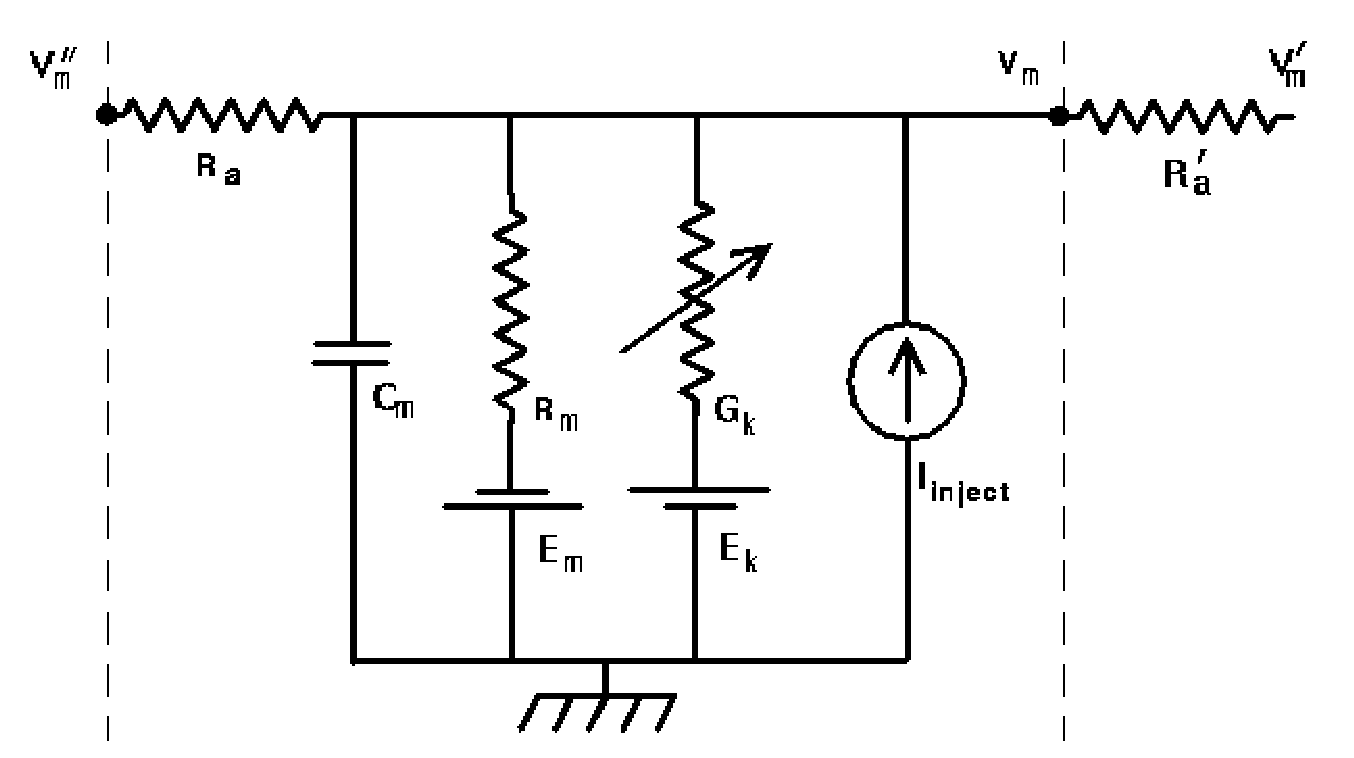
\includegraphics[height=4cm,
    angle=0]{./images/one_compartment_neuron.eps}}
\caption{En electronic circuit equivalent of a single compartment in the nerve
cell}
\label{fig:one_compartment_neuron}
\end{figure}


A model of a Purkinje cell from the cerebellum made with GENESIS by De Schutter
and Bower. It has 4550 comparments and 8021 active conductances ("channels"). If
you look closely, you can see that it is actually composed of many cylinders.


Why would one need to construct such a detailed model? If the goal is to
understand the way that individual neurons "compute", rather than to implement
some abstract model of "neural computation", there is no way to avoid
understanding the way that the dendritic structure processes its many inputs.
After achieving this understanding with a structurally realistic model, it might
be possible to produce a simpler "ball and stick" model that will function
equivalently in a large network model.


If we ultimately want a simple, computationally efficient neuron model that can
be used in simulations of very large neuronal networks, it is better to throw
out details after proving that they aren't significant, rather than just hoping
that we didn't omit something important at the outset.

\subsection{GENESIS G-3: Neurospaces project.}
\label{sec:GENESIS-3.0}

\url{http://neurospaces.sourceforge.net/}


\subsection{Large single-cell models}

Large single-cell models are currently best handled by using optimizations such
as the GENESIS \verb!hsolve! object, and these are not appropriate for
partitioning with P-GENESIS (Sect.\ref{sec:P-GENESIS}).



\subsection{P-GENESIS}
\label{sec:P-GENESIS}

P-GENESIS is an extension to GENESIS to run on parallel machines to (1) speed up
the simulation of the network models, or (2) concurrently simulate multiple
models, i.e. parameter searching.

The tool adds new commands to the scripting language to enable a script running
on one processor execute remote procedure calls on other processors, and that
let a script synchronize its execution with the scripts running on other
processors. An instance of a running P-GENESIS process is
called a {\bf node}.

To use P-GENESIS, we can modify the original GENESIS script so that portions of
them may execute in parallel. 



\subsection{Books}

The first edition (1994) of the book {\it Book of Genesis} was based on GENESIS
2.0. The second edition (1998) has
\begin{itemize}
  \item   "Biochemical Kinetic Models" by U.S. Bhalla
 
  \item   "Parallel Simulation of GENESIS Models" contributed by N.Goddard and
  G.Hood (Part Two)
\end{itemize}
Online edition: \url{http://www.genesis-sim.org/GENESIS/iBoG/iBoGpdf/}




\section{PyNN}
\label{sec:PyNN}

PyNN serves as an interface that can write a simulation script once (in Python
language), and then run the code by calling an appropriate simulation software
(currently NEURON, NEST, PCSIM, Brian and the Heidelberg VLSI neuromorphic
hardware). Each simulator has different optimizations, so the most appropriate
simulator can be chosen for a given modelling task \citep{davison2009}.

% PyNN is such an interface, making it possible to write a simulation script
% once, using the Python programming language, and run it without modification
% on any supported simulator
PyNN increases the productivity of neuronal network modelling by providing
high-level abstraction, by promoting code sharing and reuse, and by providing a
foundation for simulator-agnostic analysis, visualization and data-management
tools.


\section{OpenWorm}
\label{sec:OpenWorm}

\url{http://www.artificialbrains.com/openworm}

\section{RuleMonkey}
\label{sec:RuleMonkey}


\section{Smoldyn}
\label{sec:Smoldyn}

Smoldyn is for stochastic simulation of spatial bio-chemical networks and
intracellular systems
\begin{enumerate}
  \item continuous space, fixed time-step

  \item off-lattice particle-based model (core)
  and recently on-lattice model
  
  
  \item molecules and surfaces 
  
  \item diffusion, surface interactions, reactions
\end{enumerate}
\url{http://www.smoldyn.org/about1.html}

Compared to the popular MCell (Sect.\ref{sec:MCell}) and ChemCell
(Sect.\ref{sec:ChemCell}) simulators, we found that Smoldyn was in many cases
more accurate, more computationally efficient, and easier to use


\section{SNNAP}
\label{sec:SNNAP}

SNNAP (Simulator for neural networks and action potentials) is written in Java
and runs on most computers. Moreover, SNNAP provides a graphical user interface
(GUI) and does not require programming skills.

\section{SpiNNaker (hardware-based)}
\label{sec:SpiNNaker}


\url{http://www.artificialbrains.com/spinnaker}

SpiNNaker is a contrived acronym derived from Spiking Neural Network
Architecture. The machine will consist of 65,536 identical chip.
\begin{itemize}
  \item all chip are identical 18-core processors, giving it 1,179,648 cores in
  total.
  
  SpiNNaker is thus about 1\% the size of the human brain, which has about 85\%
  billion neurons.
  
  \item each chip is connected to six neighbours, forming a toroidal
  network.
  
  \item each processor on a chip has on-board router to form links with its
  neighbours, as well as its own 128 MB of memory to hold synaptic weights.
  
  \item each processor is an ARM968 manufactured using a 130 nm process.
  
\end{itemize}

Rather than implement one particular algorithm, SpiNNaker will be a platform on
which different algorithms can be tested.
\begin{itemize}
  \item  The topology of the simulated neural network, however, is completely
  independent of the physical hardware design. In a typical simulation a neuron would have around 1,000 synapses. 
  
  \item  Each processor core is programmable.
It can implement any model that fits in its 32 kB instruction memory. 
\begin{verbatim}
input ---> (model-neuron) ---> output
\end{verbatim}
  
  \item Each spike is a 40-bit packet containing a 32-bit identifier of the source
neuron. 
  
\end{itemize}


\section{SpringSaLaD}
\label{sec:SpringSaLaD}

\url{http://www.ccam.uchc.edu/ccam-software/}

SpringSaLaD is a particle-based, stochastic, biochemical simulation platform
most suitable for modeling {\bf mesoscopic systems}, which are far too large to
be modeled with molecular dynamics but which require more detail than obtainable
with macroscopic continuum models. In SpringSaLaD, molecules are modeled as a
collection of impenetrable spheres (called "sites") linked by stiff springs. The
sites are intended to represent mesoscopic protein domains, such as an SH2
domain or a catalytic domain, and each site can be associated with a number of
biochemical states, such as "active" or "inactive" for a catalytic domain.
SpringSaLaD supports the full array of typical biochemical reactions:
zeroeth-order reactions which model particle creation, a variety of first-order
reactions such as particle decay, dissociation, and state transitions, and
second-order reactions between sites for bonding reactions.


 In general, SpringSaLaD is best used to model mesoscopic particles (diameters
 of 1 - 10 nm, which could represent a functional protein domain), moderately
 sized systems (10 - 10,000 particles), and times scales on the order of 1
 second, but no actual restriction is set on size or scale of the simulated
 system.
 Example:  ligand-mediated receptor clustering, where coarse-grained
 particle-level interactions are required but atom-level information is not of
 interest.
 
\section{STOCHSIM (2013)}
\label{sec:STOCHSIM}

STOCHSIM is a stochastic simulator for biochemical reactions.

The particles are represented as individual software objects which react
according to probabilities derived from concentrations and rate constants.

\url{https://sourceforge.net/projects/stochsim/}

\section{VCell - VirtualCell}
\label{sec:VirtualCell}


The graphical user interface enable users to build and visualize full molecular
details of species and reaction rules
\begin{enumerate}
  
  \item Different applications: spatial, nonspatial, deterministic, stochastic
  
  \item  Rule-based models can span multiple compartments.
  
  
  \item Reactions and rules can be mixed and can both be visualized in the
  Reaction Diagram.
  
  \item  
\end{enumerate}


\url{http://vcell.org/run-vcell-software}

\subsection{Versions}

VCell 6.0+ beta
\begin{enumerate}
  \item  Rule-based modeling
  
New BioModel Physiology allow specification and visualization of: Molecules
(with multiple binding sites and states), Observables and Reaction Rules.

  \item Network-free using NFSim (Sect.\ref{sec:NFSim}): when a reaction network
  is too large or is unbounded, rule-based models may spawn network free (aka particle-based) stochastic simulations.
  
  \item Simple 3D visualization tool based on the VTK standard and the Visit
  visualization framework.

 
\end{enumerate}


VCell 5.3
\begin{enumerate}
  \item Generalized compartmental modeling: compartments no longer need to be
  completely enclosed within other compartments. 
  
  For example, this allows for modeling of multicellular tissues, intercellular
  transport through gap junctions and the influence of cell surface receptor
  activation on nuclear events without requiring specification of intermediate
  signals through the cytosol.

 
 \item Generalized unit management: Model-specific unit systems and model unit
 translation capabilities.  
 
 \item Compatible with SBML (Sect.\ref{sec:SBML}):

 VCell is compatible with 323 of the curated models from the BioModels.net
 database; these can be directly uploaded into VCell from within the VCell
 interface. All non-spatial VCell models can be exported as fully-compliant
 SBML.
 
 
 \item Redesigned interface and improved handling of Events in non-spatial
 Applications.
\end{enumerate}

VCell 5.2
\begin{enumerate}
  \item  Constructive Solid Geometry (building a complex geometry from simple
  shapes)
  
  \item Improved Pathway Model usability and interoperability with Pathway
  Commons, BioModels.net, and SABIO-RK databases.
  
  \item Hybrid spatial stochastic solver combines particle based dynamics of
  certain species with reaction diffusion equations of other species within a
  single simulation. (For example, local activation of channel activity may be
  modeled stochastically while the flux of ions through the channel may be
  simulated deterministically.)   
\end{enumerate}

VCell 4.0 (2005)
\begin{enumerate}
  \item major redesigned of UI: MDI (multiple-document interface)
  \item each BioModel can have multiple Applications
  \item Database manager
\end{enumerate}

\subsection{Run locally}

By default, once you login, you can access your models stored on UConn servers,
and will be executed there. There is a limit on the amount of data storage.

You can save a model by using the Export menu item under the File menu. The
default file format is .vcml, which will allow you to save a complete version of
the model locally on your computer hard drive. This does not save simulation
results, however.

To run the model locally, by
\begin{enumerate}
  \item export the model to local machine via Quick Run button
  (the blue button all the way on the right of the tool bar in the Simulations
  window) in the Simulation tab
 
\end{enumerate}

To save the simulation results from a local run, you can use the Table View for
non-spatial simulation results, right click and choose copy all, then paste into
a spreadsheet program to transfer all the data. 

For Spatial Simulation results, use the various choices on the Export Data
window of the results viewer (consult the help pages for details on the various
export choices). Simulation results will be lost unless you go through this
process of exporting data. Also, one limitation of not using the server and the
VCell database is that you will only be able to run one simulation at a time.

\url{https://groups.google.com/forum/#!topic/vcell-discuss/piCoYh093iM}

\subsection{Rule-based (6.0+)}
\label{sec:VirtualCell-Rule-based}

The popular rule-based software tools (Sect.\ref{sec:Rule-based-modeling})
BioNetGen (Sect.\ref{sec:BioNetGen}) and NFSim (Sect.\ref{sec:NFSim}) provide
powerful modeling and simulation capabilities at the cost of learning a complex
scripting language which is used to specify these models.

VCell provides new graphical rule-based model specification with existing
simulation engines. A set of rules can be simulated with Network-Free Simulator NFSim
(Sect.\ref{sec:NFSim}). 'Molecular Anchors' in rule-based models that keeps
membrane-bound receptors attached to the membranes (Schaff et al., 2016).

A mathematical model can be built integrating explicit reaction networks with
reaction rules.



\subsection{How to create a model using BioModel workspace}

\textcolor{red}{\bf Step 1}:
A model (in BioModel workspace) can be created by first building the geometry
\begin{itemize}
  \item single compartment in 3D, 2D, 1D or 0D (where all diffusive processes
  are approximated as instantaneous).


For 0D compartments, the user is asked to specify the volume and surface area of
each structure that was defined in the Physiology; this is important for the
proper calculation of concentrations associated with molecules that move between
the membrane and an adjacent volumetric compartment.
  
  \item multiple compartments with membranes
  
  
  \item 3D geometrical structure with membranes
\end{itemize}

\textcolor{red}{\bf Step 2}: add species.
\begin{itemize}
  \item Species (including ions, channels, receptors) can be added
  
\end{itemize}

\textcolor{red}{\bf Step 3}: add reactions (Sect.\ref{sec:reaction-VCML})
\begin{itemize}
  \item {\bf SimpleReaction}: within a compartment or membrane 
  
  
  \item {\bf FluxReaction}: flux reaction on a membrane.
\end{itemize}

\textcolor{red}{\bf Step 4}: applications (simulation)
\begin{enumerate}
  \item {\bf deterministic}
  \begin{itemize}
    \item ODE
    
    \item PDE
  \end{itemize}
  
  \item {\bf stochastic}
  
  \begin{enumerate}
    \item Gibson-Bruck Next Reaction method
    (Sect.\ref{sec:Gibson-Bruck-Next-Reaction-method})

  \end{enumerate}

While the algorithm simulates events as they randomly occur, the user can specify
regular time intervals at which the results should be displayed.


\textcolor{red}{How to convert deterministic model to stochastic?}
One problem with deriving stochastic applications from a general VCell BioModel
is that the reaction kinetics are introduced in the model as deterministic
(Sect.\ref{sec:Kinetics-VMCL}).
The unambiguous interpretation of these in terms of Poisson stochastic processes
is possible only for mass-action kinetics, and even in this case, the reversible
reactions should be decoupled into two separate processes.

SOLUTION: an analyzer tool has been developed that automatically maps
mass-action reaction rates to probabilistic propensities, and facilitates the
mapping of other reactions.
It parses the rate expression, whether the mechanism might be a combination of
individual Poisson processes (for example, if they are passive fluxes). It then
informs the user: (i) which of the mechanisms with kinetics other than mass
action can be directly translated into probabilistic propensities (and asks
permission to do it automatically), and (2) which of the mechanisms have to be
recast manually by the user into a combination of one or more mass-action types.

NOTE: Exact stochastic simulators may be ineffective for systems that involve
significantly different time scales ('stiff' systems). A number of hybrid
algorithms [15,16], which allow a user to make an appropriate compromise between
accuracy and efficiency, are currently being tested in VCell 4.5.

  \item {\bf ODE-only parameter search}
(Sect.\ref{sec:parameter-search-VCell}).

  
  \item {\bf Convert ODE to PDE}
  
The automatic translation of a compartmental Application into a spatial Application simply by
changing the Geometry to a spatially-resolved one allows users to test the results of the
compartmental simulations in a spatial contex

\end{enumerate}

\textcolor{red}{\bf Step 5}: initial conditions
\begin{enumerate}
  \item volume and surface area: 
  
VCell / Applications / Geometry / Structure Mapping

  \item initial values
  
VCell / Applications / Specifications / Species
\end{enumerate}


\subsection{How to create a a model using MathModel workspace}

The MathModel from BioModel (Sect.\ref{sec:BioModel-VCML}) is only read-only;
and is automatically generated from BioModel.

Before you can edit (e.g. to make a more complicated model), it must be
transferred to the MathModel workspace and saved as an independent mathematical
model. You can, but rarely you want to use (as it is hard to ensure the created
model working properly and for its physical correctness), also use the MathModel
workspace to create a mathematical model from scratch.




\subsection{Exchange models}

VCell uses VCML file format (Sect.\ref{sec:VCML}), which, under certain
conditions, can be exported to SBML, CellML, and Matlab for exchanging of VCell
model data with other software tools.

NOTE: neither CellML or SBML currently support spatial modeling and they have
limited support for the abstractions used in VCell for membrane transport.
Additionally, SBML does not support electrophysiological phenomena.

\verb!BioNetGen@VCell service! enables reading rule-based model from BioNetGen
input file (Sect.\ref{sec:BioNetGen}) and perform reaction network generation
and time courses simulation. While automatic generation of all required species
and reactions defined by some sets of rules is guaranteed to be accurate, it can
nevertheless lead to reaction networks that are too large to be simulated.

\subsection{Flux}

Sect.\ref{sec:flux-VCML} describes the flux (with taking into account the
surface-membrane effect or none)

When membrane-surface and/or volume potentially contribute the amplitude of this
flux, we needs to define using Flux RX tool (two yellow half-circles).
This is called trans-membrane flux and 
transmembrane fluxes are treated as flux densities (uM.um.s-1 or
molecules.um-2.s-1) and defined specifically on membranes.  

\begin{verbatim}
1) in fully resolved spatial models (where the membrane is explicitly
represented as a boundary surface), this flux density will show up as a flux
boundary condition in the reaction-diffusion equation for the flux carrier. 
Here the volumes and surface areas come from the geometry (actually the
computational mesh).    


2) in a partially resolved spatial model (where the membrane is distributed as a
surface/volume ratio and SR lumen is a volume fraction of cytoplasm), the
surface/volume ratios and volume fractions are automatically added to the
mathematical system (you don't need to add them).  Here the volume fractions and
surface/volume ratios are defined in Application->Geometry->Structure Mapping for each compartment.    


3) in a non-spatial multi-compartmental model (where nothing is spatially
resolved), the absolute sizes of each compartment are specified in the
Application->Geometry->Structure Mapping and the surface/volume ratios and
volume fractions are automatically included in the generated math.    

\end{verbatim}


So, the "vcell way" is to translate your "net flux" reactions (where you
explicitly handle volume fractions) into local "flux density" reactions mapped
to membranes, which means you introduce SR lumen, SR membrane, and is simplest
to think of as a single-channel flux multiplied by the local "open" channel
density.


There are some recent public VCell cardiac myocyte BioModels from Ronghua Yang
(VCell userid "RonghuaY") which may be of interest (within VCell client - look
in "public" folder of VCell BioModel database under user "RonghuaY" ).  These
models are much more comprehensive, but include electrophysiological protocols
as well as events (to modulate channels at given times).

\subsection{dimensionless unit}

A dimension-less unit is a unit of '1'.


\subsection{Gating variable (0<g<1)}

In VCell, any entities must be a 'species'; and the use of "a molecular species"
to represent a gating variable is a common modeling hack which brings with it
inappropriate units.

\begin{verbatim}
VCELL:
In the future, we will add more general "variables" at the level of physiology
for exactly such things; it is on our TODO list. 
\end{verbatim}

NOTE: As a 
\begin{itemize}
  \item  membrane-species, the unit is '\verb!molecules.um^-2!'
  \item compartment-species, the unit is '\verb!uM!'.
\end{itemize}

If you want to make the model more tidy, you can introduce a new parameter
"\verb!m_o_gate = 1.0 * m_o!" and force its unit to be dimensionless "[1]"

then, in your kinetic laws, use "\verb!m_o_gate!" instead of "\verb!m_o!" and it
will treat them as dimensionless gating variables within your expressions.





\subsection{Event/Trigger/Reset}

\begin{verbatim}
Using events (Application->Protocols->Events) you can reset variables or
parameters at times which are triggered as follows: 


1) at a single time 

2) when a variable exceeds an upper limit

3) when a variable drops below a lower limit

4) at a list of times

5) at N times from t_start to t_end (linear range)

6) at N times from t_start to t_end (log range)

7) when a general condition becomes true (user defined expression)


I suppose a Poisson rate could be added to this list without too much trouble. 
Using option (5) you can easily specify a 1Hz periodic event. 
\end{verbatim}



\section{URDME}
\label{sec:URDME}

\url{http://urdme.github.io/urdme/}

URDME is a general software framework for modeling and simulation of stochastic
reaction-diffusion processes on unstructured, tetrahedral and triangular meshes.
It needs Compsol Multiphysics 4.0 (Sect.\ref{sec:finite-element-COMOSOL}).

\section{Finite-element modeling}
\label{sec:finite-element-modeling}


Generate neuron mesh from morphology
\begin{verbatim}
LiveMesh: 
https://infoscience.epfl.ch/record/218021

Neurite:  
\end{verbatim}

Finite-element modeling tools: 
\begin{verbatim}
    Elmer https://www.csc.fi/web/elmer
    Kratos http://www.cimne.com/kratos/
    OpenFoam http://www.openfoam.com/
    CaeLinux http://caelinux.com/CMS/
    Fenics: https://fenicsproject.org/
\end{verbatim}

\url{http://scicomp.stackexchange.com/questions/17504/alternatives-to-comsol-multiphysics}
\url{http://alternativeto.net/software/comsol/}


\subsection{COMSOL}
\label{sec:finite-element-COMSOL}

COMSOL Multiphysics is a general-purpose software platform, based on advanced
numerical methods, for modeling and simulating physics-based problems. 

\url{http://elib.usm.my/cgi-bin/koha/opac-detail.pl?biblionumber=88381&shelfbrowse_itemnumber=217241}

\chapter{Model Markup Language}


The challenge in defining model description (as input to a simulator) is being
addressed through several community standards (CellML, NeuroML, NineML, SBML).

\section{SBML}
\label{sec:SBML}

 Systems Biology Markup Language (SBML) is an XML-based format to represent 
 computational models of biological processes.
 Its support for spatial modeling is only available in SBML Level 3 Version 1
 Spatial format.
 
 It supports non-spatial multi-compartmental model of
 \begin{enumerate}
   \item  metabolic networks, 
   
   \item cell signaling pathways, 
   
   \item regulatory networks,
   
   \item infectious diseases,
 \end{enumerate}
 
\subsection{versions}

 VERSIONS: 
 \begin{enumerate}
   \item  SBML Level 1, Version 1 (March 2001)
   
   \item SBML Level 2 (Jul, 2002)
   
   \item SBML Level 2 Version 2 (Sept. 2006): correct limitation in previous
   version
   
   \item SBML Level 2 Version 3 (2007): with 2 new SBML editors
   
   \item SBML Level 2 Version 4 (Fall 2008)
   
   \item SBML Level 3 Version 1: It uses  a new modular base for future extension proof.
   
   \begin{itemize}
     \item  {\bf Core} (2010): significant changes in syntax, and
   constructs from Level 2 Version 4
   
Additional Level 3 packages can be layered on to this core to provide
additional, optional features.

     \item {\bf Spatial SBML Level 3 Version 1 Spatial} (2010): support spatial
     modeling
   \end{itemize}
   


     
   \item SBML Level 2 Version 5 (2015): included a number of textual (but not
   structural) changes 
 \end{enumerate}

\subsection{reading}

Open-source software infrastructure such as libSBML and JSBML


\section{VCML (0.4 then 1.0)}
\label{sec:VCML}

VCML is VCell Markup Language (*.vmcl) that is used to describe the whole model.
\begin{itemize}
  \item BioModel workspace (diagram-based of chemical reactions/diffusion)
  
VCell automatically transfer the BioModel into MathModel.
This is done by applying physics principles, such
as local mass conservation and, in the context of membrane potential, conservation of
electric charges.

The math description in the BioModel workspace is read-only in order
to maintain one-to-one correspondence with the BioModel from which the math has been
generated. 

This math description, however, can be moved to the MathModel workspace for
further editing. In this case, it becomes a standalone mathematical model with
no ties to any VCell BioModel.

  \item MathModel workspace - Sect.\ref{sec:MathModel-VCML}

\end{itemize}

VCML 0.4 is obsolete.
VCML 1.0 is being used from VCell 5.0.
\url{http://wiki.vcell.uchc.edu/twiki5/bin/view/VCell/VcmlSpec}

\begin{verbatim}
<vcml xmlns="http://sourceforge.net/projects/vcell/vcml"
Version="Beta_Version_6.1_build_3">
   <BioModel Name="CalciumSignaling_WithAdaptation-cAMP_oscillations">
   </BioModel>	
</vcml>
\end{verbatim}
VCML can have 1 \verb!<BioModel>! element (that represents a Virtual Cell
BioModel) or 1 \verb!<MathModel>! element (that represents a Virtual Cell
MathModel) as a top level element.


The XML-based file whole contents describing biological and mathematical models
and specifications for analysis (e.g. simulations) to be performed on those models. 



\subsection{-- Units}

Units in the Virtual Cell are not explicitly specified in VCML. Units for
quantities in the Virtual Cell are based on the SI unit system.

Unit support in the Virtual Cell is provided with the use of an extenal java
library from The University Corporation for Atmospheric Research (UCAR). The
ucar.units package provides support for parsing and formatting string unit
specification, converting numerical values between compatible units, and
performing arithmetic on units (such as dividing one unit by another).    


\subsection{-+- BioModel (0 or 1)}
\label{sec:BioModel-VCML}

A Virtual Cell BioModel, represented by the \verb!<BioModel>! element, consists
of 1 model represented by \verb!Model! (Sect.\ref{sec:Model-VCML}), one or
more optional experimental set-ups (or Applications) represented by
\verb!SimulationSpec! (Sect.\ref{sec:SimulationSpec-VCML}), and auxiliary
information such as \verb!<Version>! and different types of annotations.
\begin{enumerate}
  \item (Vcell annotation) an optional \verb!<Annotation>! child used to store
  useful information about a model such as any comments that the creator of the model wishes to add to
  indicate what the model represents  
  
  \item (MIRIAM annotation) For models that have MIRIAM annotation, there is an
  additional \verb!<annotation>! element which stores the MIRIAM annotation in the rdf
  format.
  
NOTE: MIRIAM (Minimum Information Required In The Annotation of Models) provide
the  service for generation of unique and perennial identifiers, in the form of URIs.
\url{https://en.wikipedia.org/wiki/Minimum_information_required_in_the_annotation_of_models}
\url{http://www.ebi.ac.uk/miriam/}
\end{enumerate}


\begin{verbatim}
 <Model Name="Abell2011_Ma2002">
 </Model>

 <SimulationSpec Name="bAP">
 </SimulationSpec>
 <SimulationSpec Name="bAP">
 </SimulationSpec>

 <Version Name="something">
 </Version>
 
 <pathwayModel>
 </pathwayModel>
 
 <relationshipModel>
 </relationshipModel>
 
 <vcmetadata>
 </vcmedata>
 
 <Annotation>
 </Annotation>
 <annotation>
 </annotation>
\end{verbatim}
 
\subsection{---- Model}
\label{sec:Model-VCML}

A Model section describes the physiology of the biological model 
\begin{enumerate}
  \item  cellular structures or compartments: one or many elements 
  \verb!<Feature>! (3D) and/or \verb!<Membrane>! (2D) compartments

NOTE: for 3D compartment, the concentration would be \verb!\mu!M; while in (2D)
the concentrations is number of molecules/$\mu m^2$.
  
  \item  species (represented by two elements for each species): -
  Sect.\ref{sec:Species-VCML} 
  
  \item reactions (zero or many) between species (in the same or across
  compartments):   Sect.\ref{sec:reaction-VCML}

  
  \item \verb!<Diagram>! : each element for one cellular structure or
  compartment (Sect.\ref{sec:Diagram-VCML})
  

  
  \item \verb!<ModelUnitSystem>!: Sect.\ref{sec:ModelUnitSystem-VCML} 
  
  \item \verb!<ModelParameters>! element: Global parameters in the Virtual Cell 
  
% are represented by the <ModelParameters> element in the <Model> element.
The \verb!<ModelParameters>! element contains a list of \verb!<Parameter>!
elements; each containing the expression for the parameter and having the
following attributes of type String : 
\begin{verbatim}
Name =  representing the name of the parameter

Role = representing the parameter role (reaction rate or 
           inward current density or user-defined)

Unit = name of the units of the parameter
\end{verbatim}

These parameters can be global consftants or functions
of other global parameters or of model species. Note: when using species in
global/model parameter expressions, the \verb!speciesContext! name (the
\verb!LocalizedCompound! name), should be used.
  
  \item and \verb!<Version>!  element (which contains necessary version information about the model). 
\end{enumerate}

\subsection{** Compartments: Feature}
\label{sec:Compartment-VCML}

Each compartment is declared as \verb!<Feature>! section.

\begin{verbatim}
<Model>

      <Feature Name="mitochondria" KeyValue="105940987"/>
      <Feature Name="outside" KeyValue="105940989"/>
      <Feature Name="ER_store" KeyValue="105940983"/>
      <Feature Name="cytosol" KeyValue="105940985"/>
</Model>
\end{verbatim}

\subsection{** Membrane: Feature}
\label{sec:membrane-VCML}


\subsection{** Global parameters: ModelParameter}

Global parameters in the Virtual Cell are defined in the section
\verb!<ModelParameters>! inside \verb!<Model>! section
(Sect.\ref{sec:Model-VCML}).

\begin{verbatim}
   <ModelParameters>
        <Parameter Name="k1" Role="user defined" Unit="tbd">2.0</Parameter>
        <Parameter Name="k2" Role="user defined" Unit="tbd">0.9</Parameter>
        <Parameter Name="k3" Role="user defined" Unit="tbd">2.5</Parameter>
   </ModelParameters>
\end{verbatim}

\subsection{** species: Compound and LocalizedCompound}
\label{sec:Species-VCML}

A species can be 
\begin{itemize}
  \item volume species (associate with a compartment): calcium, IP3
  \item membrane species (associate with a membrane): ion channel, which reflect
  surface density (i.e. )
  
  
\end{itemize}
Species can participate in reactions, fluxes, and diffusion. 

The value for \verb!Structure! attribute should map to the name for a
compartment (Sect.\ref{sec:Compartment-VCML})
\begin{verbatim}
<Model>
      <Compound Name="Calcium">
        <Annotation>Calcium</Annotation>
      </Compound>
      
      <LocalizedCompound Name="CaER" CompoundRef="Calcium"
      Structure="compartment" OverrideName="true" KeyValue="105941164"/>
       
      <Compound Name="CAR1">
        <Annotation>CAR1</Annotation>
      </Compound>
      <LocalizedCompound Name="CAR1" CompoundRef="CAR1" 
                   Structure="compartment" OverrideName="true"
                   KeyValue="105941165"/>
            
</Model>      
\end{verbatim}

A species is defined using section \verb!LocalizedCompound! for a species and
\verb!Compound! for a species context, i.e. the species in the associated
compartment type in the Virtual Cell)

NOTE: \verb!LocalizedCompound! is equivalent to Species in SBML
(Sect.\ref{sec:SBML-Species}), and Compound is roughly equivalent to SpeciesType
in SBML (Sect.\ref{sec:SBML-SpeciesType}). 

SpeciesType class of object to enable Species objects of the same type to be
related together. SpeciesType is a conceptual construct; the existence of
SpeciesType objects in a model has no effect on the model's numerical
interpretation. Unlike SBML, the number of LocalizedCompound sections should
equal the number of Compound sections.
 \url{http://sbml.org/Community/Wiki/SBML_Level_3_Core/CompartmentType_and_SpeciesType_removed}
  
NOTE: Compared to SBML, no numerical values for initial values or kinetics is
given in the \verb!<Model>! element - all numerics is given in SimulationSpec
(Sect.\ref{sec:SimulationSpec-VCML}).

\subsection{** reactions + fluxes}
\label{sec:reaction-VCML}  
\label{sec:flux-VCML}  

A chemical reaction (within a Model - Sect.\ref{sec:Model-VCML}) is represented
as \verb!SimpleReaction! for a biochemical reaction
(Sect.\ref{sec:SimpleReaction-VMCL}) and \verb!FluxStep! for a transport in the
Virtual Cell (Sect.\ref{sec:FluxStep-VMCL}).

\subsection{------ FluxStep}
\label{sec:FluxStep-VMCL}

One of the two types of reactions in VMCL (Sect.\ref{sec:reaction-VCML}).

Fluxes are associated with a single membrane and describe the flux of a single
species through that membrane, e.g. transmembrane fluxes (e.g. flux through an
ion channel). Here,  reaction on a membrane involve the species on that membrane
as well as the species present in the compartments neighboring the membrane.

The flux species must be a species that is present in both neighboring
compartments, i.e. same name.

The attributes are similar to those used in SimpleReaction
(Sect.\ref{sec:SimpleReaction-VMCL}).

\begin{verbatim}
<FluxStep Name="PF_Flux"
          Structure="nm"
          FluxCarrier="PA"
          FluxCarrierValence="0"
          FluxOption="MolecularOnly"
>
  <Modifier LocalizedCompoundRef="NP" KeyValue="12408959" />
  
  <Kinetics KineticsType="GeneralKinetics">
  </Kinetics>
  <Annotation> explain reaction here </Annotation>
</FluxStep>
\end{verbatim}

\subsection{------ SimpleReaction}
\label{sec:SimpleReaction-VMCL}

One of the two types of reactions in VMCL (Sect.\ref{sec:reaction-VCML}).

It represents reactions as a collection of related reaction steps occurring in
or near a single structure (e.g. membrane receptor binding, cytosolic calcium
buffering).

Attributes
\begin{itemize}
  \item \verb!Name! = string uniquely identify the reaction
  \item \verb!Structure! = name of the structure (compartment or membrane)
  (Sect.\ref{sec:Compartment-VCML}, Sect.\ref{sec:membrane-VCML})  in which the
  reaction takes place
  
  \item \verb!FluxCarrierValence! = charge carrier valence
  
  \item \verb!FluxOption! = if the flux option is molecular 
only, molecular and electrical, or electrical only

  \item \verb!KeyValue! = key value of the simplereaction object
\end{itemize}

Sub-blocks: indicate 
\begin{itemize}
  \item zero or more reaction participants
  \item  zero or more catalysts/modifiers 
  \item  zero or more products
  \item  kinetics of the reaction: MassAction, GeneralLumpedKinetics, \ldots
  (Sect.\ref{sec:Kinetics-VMCL})
\end{itemize} 
It must be noted that there must be at least  one reactant or one product for a
reaction.

\begin{verbatim}
<Model>

<SimpleReaction Structure="cytosol" Name="v1" 
       Reversible="true" 
       FluxOption="MolecularOnly" 
       KeyValue="105941171"
>
  <Product LocalizedCompoundRef="ACA" Stoichiometry="1" KeyValue="105941172"/>
  <Modifier LocalizedCompoundRef="CAR1" KeyValue="105941173"/>
  <Kinetics KineticsType="GeneralLumpedKinetics">
    <Parameter Name="LumpedJ" Role="lumped reaction rate" Unit="mole.s-1">(k1 * CAR1)</Parameter>
  </Kinetics>
</SimpleReaction>


</Model>


<SimulationSpec .... >
<ReactionContext>
        <LocalizedCompoundSpec LocalizedCompoundRef="ACA" ForceConstant="false" WellMixed="false" ForceContinuous="false">
          <InitialConcentration>3.39</InitialConcentration>
          <Diffusion>0.0</Diffusion>
        </LocalizedCompoundSpec>
        <LocalizedCompoundSpec LocalizedCompoundRef="CAR1" ForceConstant="false" WellMixed="false" ForceContinuous="false">
          <InitialConcentration>2.45</InitialConcentration>
          <Diffusion>0.0</Diffusion>
        </LocalizedCompoundSpec>

<ReactionSpec ReactionStepRef="v1" ReactionMapping="included"/>

</ReactionContext>
</SimulationSpec>
\end{verbatim}

\textcolor{red}{IMPORTANT:} Each SimpleReaction, needs to have a associated
section in \verb!<ReactionContext>! and \verb!<LocalizedCompoundSpec>! (to
define initial values, diffusion constant); and potential 
\verb!<MathDescription>! section (Sect.\ref{sec:MathDescription-VCML}),
with \verb!Constant!, \verb!<VolumeVariable>! section, \verb!<Function>!
section and \verb!<CompartmentSubDomain>! section. 

Inside \verb!<CompartmentSubDomain>! section, we need to define 
\verb!<BoundaryType>!, \verb!<OdeEquation>!
  

\subsection{---- Kinetics}
\label{sec:Kinetics-VMCL}

Virtual Cell supports General,  MassAction? , Henri-Michaelis-Menten
(reversible) and Henri-Michaelis-Menten (irreversible) for volume reactions and
General Mass Flux, General Current Density, Goldman-Hodgkin-Katz Permeability
and Nernst Conductance for membrane reactions.

The General kinetics type is used for arbitrary rate expressions.

\begin{enumerate}
  \item volume reaction - Sect.\ref{sec:SimpleReaction-VMCL}
  \begin{itemize}
  \item {\bf General Mass Action}
  
  \item {\bf Henri-Michaelis-Menten} (reversible)
  
  \item {\bf henri-Michaelis-Menten} (irreversible)
  \end{itemize}

  \item membrane reaction - Sect.\ref{sec:FluxStep-VMCL}
  \begin{itemize}
  \item {\bf General Flux Density} (General Mass Flux) ($\muM.\mum.s^{-1}$)
  
  \item {\bf General Permeability} ($\muM.\mum.s^{-1}$)
  
with permeability in unit of $\mum/s$
  
  \item {\bf General Current Density} (pA / $\mum^2$)
  
  \item {\bf Goldman-Hodgkin-Katz Current Density (Permeability)} (pA /  $\mum^2$)
  
with permeability in unit of $\mum/s$
  
  
  \item {\bf Nernst Conductance}

with conductance in unit of nS/$\mum^2$


  \item General Flux (molecules / s)
  
  \item General Current (pA)
  
  \item 
  \end{itemize}
\end{enumerate}
 
\subsection{** Diagram (optional)}
\label{sec:Diagram-VCML}

Describe all reactions in the associated cellular structure or compartment 
\begin{verbatim}
 <Diagram Name="cytosol" Structure="cytosol">
        <SimpleReactionShape SimpleReactionRef="JPump" LocationX="62" LocationY="91"/>
        <LocalizedCompoundShape LocalizedCompoundRef="CaS" LocationX="14" LocationY="34"/>
</Diagram>

 <Diagram Name="ER_store" Structure="ER_store">
</Diagram        
\end{verbatim}

It tells the location, the name of the compounds that involve, and the type of
rection/flux.

A \verb!<Diagram>! element represents the reaction network in a structure
(compartment) - it has shapes (icons) for localized compounds, simple and flux reactions
  

\subsection{---- SimulationSpec}
\label{sec:SimulationSpec-VCML}
\label{sec:Application-VCML}

A SimulationSpect is a representation of an Application in the Virtual Cell,
which establishes the association between a biological model, a geometry
properly mapped to the biology, initial conditions, mathematical description,
simulations and analysis.
\begin{itemize}
  \item a <Geometry> element: that stores the geometry associated with the
  SimulationSpec

  \item a <GeometryContext> element:
  
  \item a <ReactionContext> element:
  
  \item an optional <ElectricalContext> element that contains the
  <ElectricalStimuli> and the <GroundElectrode> elements for applications with electrophysiology;
  
  \item  optional CharacteristicSize which indicates the characteristic size of
  the geometry image
  

  \item a <MathDescription> element (Sect.\ref{sec:MathDescription-VCML})
  
  \item a <Simulation> element - Sect.\ref{sec:Simulation-VCML}   
  
  \item a <MicroscopeMeasurement> element
  (Sect.\ref{sec:MicroscopeMeasurement-VCML})
\end{itemize}

A number of boolean attributes that are needed to be defined

{\tiny
\begin{verbatim}
<SimulationSpec Name="CalciumSignaling_WithAdaptation_cAMP_Oscillation"
      Stochastic="false" 
      UseConcentration="true" 
      RuleBased="false"
      InsufficientIterations="false" 
      InsufficientMaxMolecules="false"
      CharacteristicSize="double" >
      
      <Geometry Name="Compartmental" Dimension="0">
        <Extent X="10.0" Y="10.0" Z="10.0"/>
        <Origin X="0.0" Y="0.0" Z="0.0"/>
        <SubVolume Name="Compartment" Handle="0" Type="Compartmental" KeyValue="105940967"/>

        <Version Name="Compartmental" KeyValue="105940963" BranchId="105940964" Archived="0" Date="08-Dec-2016 00:29:09" FromVersionable="false">
          <Owner Name="tmhoangt" Identifier="105940414"/>
          <GroupAccess Type="1"/>
        </Version>
      </Geometry>
            
//initial values or kinetics in the <Model> element - allnumeric 

//VCML 1.0
 <NetworkConstraints RbmMaxIteration="3" RbmMaxMoleculesPerSpecies="10"/>
 
 
</SimulationSpec>
\end{verbatim}
}

\subsection{MicroscopeMeasurement}
\label{sec:MicroscopeMeasurement-VCML}

\begin{verbatim}
      <MicroscopeMeasurement Name="fluor">
        <ConvolutionKernel Type="ProjectionZKernel"/>
      </MicroscopeMeasurement>
\end{verbatim}


\subsection{--- GeometryContext}

a list of <FeatureMapping> (for a volumetric compartment) and <MembraneMapping>
(for a membrane) elements.

{\tiny
\begin{verbatim}
<GeometryContext>
        <FeatureMapping Feature="mitochondria" GeometryClass="Compartment" SubVolume="Compartment" Size="1.0">
          <BoundariesTypes Xm="Flux" Xp="Flux" Ym="Flux" Yp="Flux" Zm="Flux" Zp="Flux"/>
        </FeatureMapping>
        <FeatureMapping Feature="cytosol" GeometryClass="Compartment" SubVolume="Compartment" Size="1.0">
          <BoundariesTypes Xm="Flux" Xp="Flux" Ym="Flux" Yp="Flux" Zm="Flux" Zp="Flux"/>
        </FeatureMapping>
\end{verbatim}
}

Feature represents the name of the feature (3-d compartment), Subvolume
represents the name of the subvolume, Resolved indicates if the feature is
resolved or not, Size contains the size of the feature if it is set. In
addition, the <FeatureMapping> element contains a <BoundariesTypes> element,
which contains the attributes (String) Xm, Xp, Ym, Yp, Zm, Zp - each of which
can be set to Flux or Value - positive and negative values X, Y, Z boundary
conditions.


A <MembraneMapping> element has the following attributes of type String :
Membrane represents the name of the membrane; SurfaceToVolumeRatio,
VolumeFraction, Size contain the expressions for the surface-to-volume ratio,
volume fraction and size parameters, if they are set; CalculateVoltage tag that
has values of true or false indicating if voltage should be calculated or not;
SpecificCapacitance and InitialVoltage that contain the expressions for specific
capacitance and initial voltage, if present (default values of 1.0 and 0.0
respectively).


\subsection{-+- MathModel}
\label{sec:MathModel-VCML}

MathModel is an alternative choice to BioModel (Sect.\ref{sec:BioModel-VCML}).
It has the following elements : 
\begin{enumerate}
  \item  a <Geometry> element that represents the
geometry of the model; 

  \item a <MathDescription> element that describes the mathematical system that
represents the model; (Sect.\ref{sec:MathDescription-VCML})

  \item a list of <Simulation> elements, if present; and 
  
  \item (optional) Annotation element
  
  \item a <Version> element that contains the version information for the model.
  The attributes and contents of these elements are the same as those defined
  for these elements in the BioModel.
  
\end{enumerate}


\subsection{** Simulation}
\label{sec:Simulation-VCML}

Choose the type of solver

{\tiny
\begin{verbatim}
      <Simulation Name="Simulation0">
        <SolverTaskDescription TaskType="Unsteady" UseSymbolicJacobian="false" Solver="Combined Stiff Solver (IDA/CVODE)">
          <TimeBound StartTime="0.0" EndTime="111.0"/>
          <TimeStep DefaultTime="0.1" MinTime="1.0E-8" MaxTime="1.0"/>
          <ErrorTolerance Absolut="1.0E-9" Relative="1.0E-9"/>
          <OutputOptions KeepEvery="1" KeepAtMost="1000"/>
          <NumberProcessors>1</NumberProcessors>
        </SolverTaskDescription>
        <MathOverrides/>
        <Version Name="Simulation0" KeyValue="105962449" BranchId="105962450" Archived="0" Date="08-Dec-2016 14:05:31" FromVersionable="false">
          <Owner Name="tmhoangt" Identifier="105940414"/>
          <GroupAccess Type="1"/>
        </Version>
      </Simulation>
\end{verbatim}
}

\subsection{** MathDescription}
\label{sec:MathDescription-VCML}

Using a declaritive mathematics language, we can defines parameters, independent
variables, differential/algebraic systems defined over a complex geometry
including discontinuous solutions and membrane boundaries and the description of
the task to perform on such a system.

MathDescription element is inside MathModel (Sect.\ref{sec:MathModel-VCML})
{\tiny
\begin{verbatim}
<MathModel ...>
  <MathDescription Name="Abell2011_CalciumSignaling_WithAdaptation_generated">
   //Constants
   <Constant Name="_F_">96480.0</Constant>
   
   
   //<VolumeVariable Name="ACA" Domain="Compartment"/>
  
  <Function Name="LumpedJ_v1" Domain="Compartment">(k1 * CAR1)</Function>
  
  
  <CompartmentSubDomain Name="Compartment">
  
  </CompartmentSubDomain>
  
  </MathDescription
</MathModel>
\end{verbatim}
}


\subsection{-- Version}
\label{sec:Version-VCML}

The following entities have a Version : BioModel (Sect.\ref{sec:BioModel-VCML}),
MathModel (Sect.\ref{sec:MathModel-VCML}), Model, SimulationSpec, Geometry,
MathDescription, Simulation (and hence their corresponding VCML elements will contain a \verb!<Version>! element).
\begin{enumerate}
  \item BioModel: (require) store version information for the BioModel. 
  
  \item Model: contains the version information for the model.
  
  
  \item  contains necessary version information about the math description

  \item represents the version of the geometry object (creation date
and time, key value in the database, description of geometry, etc) 
  
\end{enumerate}

\verb!<Version>! : has
\begin{itemize}
  \item Name = string
  
  \item KeyValue = database table key value
  
  \item BranchID = integer, a marker for a group of related versioned models 
  
NOTE:  All entities with the same branchId are versions of the same
  model. 
  
  \item Date = (string: "dd-MM-yyyy HH"mm:ss" format) date of last save of the
  entity,
   
  \item FromVersionable : a boolean that represents if the entity is
  versionable. 
  
  \item \verb!<ParentSimRef>! : hold the keyvalue of the parent simulation
  
  This element is present only if the versionable
  entity is a Simulation.  This keyvalue allows the results to be obtained from
  the original (parent) simulation).
  
  \item Archived: It can take one of 3 values
  
  (Note: a value of '2' represents Unchanged which is not used any longer).
  \begin{itemize}
    \item     : '0' represents Current which is the
   default/normal flag setting;
    
    \item  '1' represents Archived which prevents users
   from deleting the entity; 
   
   \item '3' represents Publish which indicates that the
   model/entity has been archived and published (in extenal publications) and is
   used internally to deter administrators from deleting the model from database. 
   
   \end{itemize}    
\end{itemize}

\subsection{ModelUnitSystem (VCML1.0)}
\label{sec:ModelUnitSystem-VCML}

\begin{verbatim}
<Model>
<ModelUnitSystem 
     VolumeSubstanceUnit="mole" 
     MembraneSubstanceUnit="mole"
     LumpedReactionSubstanceUnit="mole" 
     VolumeUnit="litre" 
     AreaUnit="m2"
     LengthUnit="m" 
     TimeUnit="s"/>
</Model>
\end{verbatim}

\subsection{pathwayModel (VCML 1.0)}
\label{sec:pathwayModel}

{\tiny
\begin{verbatim}
<pathwayModel>
 <rdf>
 
        <DiagramObjectsID xmlns="">BIOMODEL_ACA</DiagramObjectsID>
 
      <bp:PhysicalEntity rdf:nodeID="BIOMODEL_mw7cb2644a_384a_4bbb_93fd_fd686e01d7cb">
          <bp:name rdf:datatype="http://www.w3.org/2001/XMLSchema#string">STIM_DROME</bp:name>
          <bp:xref rdf:nodeID="uniprot_P83094"/>
        </bp:PhysicalEntity>
        
        <bp:BiochemicalReaction rdf:nodeID="BIOMODEL_v7">
          <bp:name rdf:datatype="http://www.w3.org/2001/XMLSchema#string">v7</bp:name>
          <bp:xref rdf:nodeID="go_GO:0045858"/>
        </bp:BiochemicalReaction>        


        <bp:UnificationXref rdf:nodeID="GENE_ONTOLOGY_0051209">
          <bp:db rdf:datatype="http://www.w3.org/2001/XMLSchema#string">GENE_ONTOLOGY</bp:db>
          <bp:id rdf:datatype="http://www.w3.org/2001/XMLSchema#string">0051209</bp:id>
        </bp:UnificationXref>
        
        <bp:PhysicalEntity rdf:nodeID="BIOMODEL_mwaf195932_a72c_4552_8cf2_b349b15d39c4">
          <bp:name rdf:datatype="http://www.w3.org/2001/XMLSchema#string">Q9V4C7_DROME</bp:name>
          <bp:xref rdf:nodeID="uniprot_Q9V4C7"/>
        </bp:PhysicalEntity>
        
        <bp:SmallMolecule rdf:nodeID="BIOMODEL_excAMP">
          <bp:name rdf:datatype="http://www.w3.org/2001/XMLSchema#string">excAMP</bp:name>
          <bp:xref rdf:nodeID="chebi_CHEBI:17489"/>
          <bp:xref rdf:nodeID="kegg.compound_C000575"/>
        </bp:SmallMolecule>  
        
        <bp:RelationshipXref rdf:nodeID="uniprot_Q01386">
          <bp:db rdf:datatype="http://www.w3.org/2001/XMLSchema#string">UNIPROT</bp:db>
          <bp:id rdf:datatype="http://www.w3.org/2001/XMLSchema#string">Q01386</bp:id>
        </bp:RelationshipXref>                      
 </rdf>
</pathwayModel>
\end{verbatim}
}

\subsection{vcmetadata}
\label{sec:vcmetadata-VCML}

\begin{verbatim}
<vcmetadata>


</vcmetadata>
\end{verbatim}





\section{NeuroML}
\label{sec:NeuroML}

Sect.\ref{sec:NeuroML-file-format}

\section{CellML}
\label{sec:CellML}


\section{BioPax, SyBiL}
\label{sec:BioPax}
\label{sec:SyBiL}

Pathway data captures our understanding of biological processes; yet the current
fragmentation of pathway information across many databases with incompatible
formats presents barriers to its effective use.

{\bf BioPAX} was developed to solve that using OWL/XML.

SyBiL is short for Systems Biology Linker. Biological pathways, reaction and
signaling networks are made publicly availabel in formats standardized to the
Biological Pathway eXchange format (BioPAX).  

\url{http://vcell.org/biopax/}

\subsection{conversion}

BioPAX to SBML: BioPAX2SBML 
\url{https://www.ncbi.nlm.nih.gov/pubmed/22923304}

\section{BioNetGen language (BNGL)}
\label{sec:BNGL}


\section{BioModel databases}
\label{sec:BioModel-database}

BioModels Database is a repository of computational models of biological
processes using MIRIAM standard (minimum information requested in the annotation
of biochemical models. Models described from literature are manually curated and
enriched with cross-references.


Old: \url{http://biomodels.net}

Current:\url{https://www.ebi.ac.uk/biomodels-main/publmodels}

\section{Jarnac}
\label{sec:Jarnac}

Jarnac is a language for describing and manipulating cellular system models 
\url{http://sbw.kgi.edu/software/jarnac.htm}

Jarnac is based on a simple control language, similar to the Basic language and
supports many of the constructs one would expect,  for loops, conditionals,
while/do and repeat/until. It supports at least 7 different data types,
including integers, floats, Booleans, strings, vectors, matrices and lists.
Jarnac also supports user defined functions and external modules.

There is built-in computational support for: Dynamic simulation (using LSODAor
CVODE integrator), steady state snalysis using the NLEQ solver, simple stability
analysis (eigenvalues, using IMSL library), matrix arithmetic (All the main
operators including things like transpose, det etc, using IMSL library),
Metabolic Control Analysis (All steady state control coefficients and
elasticities), Metabolic atructural analysis (Null space and conservation
relation analysis with others to follow), stochastic Simulation (using standard
Gillespie method).

\chapter{Output data experimental ephys-recording file format }

Proprietary formats being closed source in general result
in software lock-in and hinder data sharing. One approach
to address this issue involves software tools to convert data
from one format to another.

In addition to researcher expertise in designing the experiment, data collection
in experiments is expensive. All experimental data are unique, and cannot be
re-generated.

\section{Neo: (Garcia et al. 2014)}
\label{sec:Neo-library}

neo.io can be seen as a pure-Python and open-source Neuroshare replacement
(Sect.\ref{sec:Neuroshare-API}).

The Neo io module aims to provide an exhaustive way of loading and saving
several widely used data formats in electrophysiology.
Currently, there are 3 families of IO modules:
\begin{enumerate}
  \item for reading closed manufacturers' formats (Spike2, Plexon, AlphaOmega, BlackRock, Axon, ...)

  \item for reading(/writing) formats from open source tools (KlustaKwik, Elan,
 WinEdr, WinWcp, PyNN, ...)

   \item for reading/writing Neo structure in neutral formats (HDF5, .mat, ...)
   but with Neo structure inside (NeoHDF5, NeoMatlab, ...)
\end{enumerate}
\url{http://neo.readthedocs.io/en/0.4.0/io.html}


% Garcia, S., Guarino, D., Jaillet, F., Jennings, T., Propper, R.,
% Rautenberg, P.L., Rodgers, C.C., Sobolev, A., Wachtler, T., Yger,
% P., & Davison, A.P. (2014). Neo: an object model for handling
% electrophysiology data in multiple formats. Frontiers in Neuroinformatics,
% 8, 10.
\section{INCF (2014)}
\label{sec:INCF-2014-format}

A recent initiative by the International Neuroinformatics Coordinating Facility
(INCF) attempts to develop a standard format for sharing data from
electrophysiology experiments (INCF 2014b).



\section{Neuroshare API (G-Node 2004)}
\label{sec:Neuroshare-API}

Neuroshare.org is a site created to support the collaborative development of
open library and data file format specifications for neurophysiology and
distribute open-source data handling software tools  for neuroscientists.

The purpose of this Application Programming Interface (API) standard is to
define a common interface for accessing neurophysiology experiment data files.
The Neuroshare API is available as a C library and as a MATLAB (The Mathworks
Inc.) extension. 
 
\begin{enumerate}
  \item trial start/stop marker
    
  \item stimulation information
  
  \item reward information
  
  \item position information
  
  \item force information
  
  \item EEG data
  
  \item EMG data
  
  \item extracellular spike
  
  \item embedded comments
\end{enumerate}

\begin{verbatim}
Load Needed Library;

Repeat for Each Neural Data File,

    Open Neural Data File;

          Get General File Information;

          Query Number of Entities;

          For Each Entity,
                Get Entity Type;
                Get Type Specific Entity Information;

          Repeat Main Operational Loop,
                Determine Entities of Interest;
                Search for Needed Indexes of Relevant Entities;
                Retrieve the Data for the Relevant Entities;
                Do Application-Specific Processing and Display;
          While Still Interested;

While Neural Data Files Remain;

Close All Neural Data Files;

Unload Library;
\end{verbatim}

\url{http://neuroshare.sourceforge.net/index.shtml}

\section{EDF (2003)}
\label{sec:EDF-format}

(EDF (Kemp and Olivan
2003), 

\section{SignalML (2004)}
\label{sec:SignalML-format}


SignalML (Durka and Ircha 2004), 

\section{XCEDE (2012)}
\label{sec:XCEDE}

XCEDE (Gadde et al. 2012), 

\section{BioSignalML (2011)}
\label{sec:BioSignalML-format}

BioSignalML (Brooks et al. 2011), 

\section{NDF (2010)}
\label{sec:NDF-format}

NDF (Liang et al. 2010))

\chapter{Output data simulation file format }

Despite many points of overlap, simulation data has rather different
requirements compared to data from wet experiments. In simulations data are
generated, whereas in experiments data are collected.

\section{NSDF (2014)}
\label{sec:NSDF-format}

Ray et al. (2014) proposed a format for storing and sharing data from computer
simulations in neuroscience, based on HDF5.
The proposed format is general enough to accommodate the variety of data
generated from the wide range of modeling approaches and algorithms used in
computational neuroscience.

It is designed to be self-documenting so that analysis and visualization tools
can operate upon it without additional implicit or explicit knowledge of the
data source or content.
\begin{enumerate}
  \item Python module: \url{https://
github.com/nsdf}

facilitates reading and writing of NSDF files

  \item 
\end{enumerate}


Format:
\begin{enumerate}
  \item level 0 : root '/'
  
  \item level 1: 3 predefined groups
  
\verb!/data!: store all data (NOTE: Data do not have much meaning without
information about their origins. which is label of the data)



\verb!/map!: (what the labels of the data are) store the mappings between data
datasets and sources, as well as sampling times;

\verb!/model!: (components that generated the data) storing information
about the model from which the data were generated.
\end{enumerate}

\subsection{performance }

The data component (/data group) is the most demanding for speed and space.

It is relatively easy to define efficient formats for \verb!static! data and
\verb!uniform!ly sampled time-series.

Non-uniform and event data present a multitude of trade-offs, and further the
underlying software support is itself evolving



\subsection{/map/ level-2 names: source, data}
\label{sec:NSDF-format-/map/-level-2}

The mapping between the datasets and the sources is stored under /map in a
compound dataset with two fields, \verb!source! and \verb!data!, storing the
source-uid and the reference to the dataset respectively.

The arrays inside \verb!/map/source! are dimension scale arrays
(Sect.\ref{sec:dimension-scale}).


\subsection{/data/ level-2 names: static, uniform, nonuniform, event}
\label{sec:NSDF-format-/data/-level-2}

There are 4 pre-defined names for groups under /data in an NSDF file: static,
uniform, nonuniform, and event

\begin{enumerate}
  \item \verb!static! data, e.g. model parameters and connectivity
information are static.


  \item \verb!uniform! data or \verb!nonuniform! data, e.g.
  Time series values, such as membrane potential in the Hodgkin-Huxley model,
  may be sampled at uniform or non-uniform interval
  
  \item \verb!event! : spiking data are most efficiently stored as events

 
\end{enumerate}

\subsection{/data/uniform/ level-3 names: }
\label{sec:NSDF-format-/data/uniform/-level-3}

The /data/uniform group has subgroups representing population level groups
(level 3).

Each variable recorded from multiple elements in a population can be wrapped
into a 2D dataset where each row corresponds to one element.


Example, if we record membrane potential from neurons n1, n2, . . . , nP , at
equally spaced time points \verb!t1, t2, .., tQ!: then we store as 2D-array
Vm with \verb!Vm[i,j]! representing the value recorded from neuron ni at time
tj. Two options to store the time points (we recommend to use only one approach
in a given dataset)
\begin{enumerate}

  \item only store \verb!tstart! and \verb!dt! timestep: 
  
  the start time of simulation and the sampling interval in the dataset as
  attributes tstart (t1) and dt (ti+1-ti ), respectively


  \item store the list of time points (t1, t2, . . . , tQ) explicitly in a
  dataset \verb!/map/time! group, and attach it to the column dimension of Vm as
  a dimension scale named \verb!time!

\begin{verbatim}
/map/
   |
   /nonuniform/
       |
       /neuronB array 
          row-1 : dend
          row-2 : soma


/map/
   |
   /time/
       |
       /tpoints array 
          col-1 : t1, t2, ..., tM
\end{verbatim}

\end{enumerate}
In both cases, the source uids are saved as source dimension scale attached to
the row dimension in /map/uniform.

\subsection{/data/nonuniform/ level-3 names: }
\label{sec:NSDF-format-/data/nonuniform/-level-3}

neuronB is simulated under variable time step and the variables are recorded at M nonuniform
time points.

the transmembrane current Im recorded for this
neuron is stored in /data/nonuniform/; also, the sources
are stored in /map/nonuniform/neuronB (information for each row); and
/map/time/tpoints (information for time).

\begin{verbatim}
/data/
   |
   /nonuniform/
       |
       /neuronB 
         |
         /Im array
         row-1: dend[1], ..., dend[M]
         row-2: soma[1], ..., soma[M]
\end{verbatim}

\begin{verbatim}
/map/
   |
   /nonuniform/
       |
       /neuronB array 
          row-1 : dend
          row-2 : soma


/map/
   |
   /time/
       |
       /tpoints array 
          col-1 : t1, t2, ..., tM
\end{verbatim}

\subsection{/data/static/ level-3 names: }
\label{sec:NSDF-format-/data/static/-level-3}

The connectivity information, i.e., pre and post synapses and their
synaptic weights are stored under /data/static

\begin{verbatim}
/data/
   |
   /static/
       |
       /cells/
          |
          /synapses  array
           meta{pre, post, weight}
               {axonA, somaB, 7}
               {axonB, somaA, 5}
             
\end{verbatim}

The corresponding source specification, or uid of the source of this data, is
stored under /map/static.

The entries in data and map are connected via a dimension-scale which
establishes a row-wise mapping between data and map.

A similar pairing of data and map is present for time-series
data.

\subsection{/data/\ldots/ level-3 names: compartment, channel}
\label{sec:NSDF-format-/data/-level-3}

Inside one of the names in level-2 of \verb!/data! group
(Sect.\ref{sec:NSDF-format-/data/-level-2}), we have another set of pre-defined
names: \verb!channel!, \verb!compartment!.

The goal is to group of the data belonging to the same type together, e.g.
channel current data. 

Each dataset has a dimension scale representing the sampling times associated
with it. Moreover, the unique
identifier of the data source must be stored in the dataset
attribute \verb!source!.

\subsection{/data/\ldots/\ldots/ level-4 data: real-data}
\label{sec:NSDF-format-/data/-level-4}


A 2-dimensional HDF Dataset at level 4, or can be stored as
individual 1-dimensional datasets at level 5, in which
case the level 4 node is an HDF Group.

Data do not have much meaning without information about
their origins.

what the labels of the data are

When the data are stored in a 2D dataset, {\it each row corresponding to one
source}, the list of sources is attached as a dimension scale which is just
another dataset storing the list of source ids.




\subsection{/data/\ldots/\ldots/ level-4 names: name-of-variable}
\label{sec:NSDF-format-/data/-level-4}

We can decide to store values for a number of variables from the model
components in a group. Each such variable can be represented
by a separate node at level 4.

Then, the data can be stored as individual 1-dimensional datasets at level 5, in
which case the level 4 node is an HDF Group.

\subsection{/data/\ldots/\ldots/\ldots/ level-5 data: real-data}
\label{sec:NSDF-format-/data/-level-4}

If level-4 is a group name, then level 5 is the real 1-D data.



\subsection{/model/modeltree/}
\label{sec:NSDF-format-/model/modeltree}

The hierarchical model
structure is stored as a subtree of /model/modeltree
with groups representing model components

Additional attributes are provided for unique identifiers
(uid) and ontological terms (ontology).

uid can be a URI, XML path or any string that can uniquely identify the data
source within the file context.

The ontological terms (short form or full URI) can be used for identifying the
type of the component based on some predefined ontology like the Computational
Neuroscience Ontology (Le Franc et al. 2012) or Gene Ontology Database
(Ashburner et al.
2000).

Each group in the model tree can be linked to the data
recorded from its members through the map attribute, which
can be used by software applications to efficiently identify
the data collected from this model component or its subcomponents.

